\documentclass[a4paper,twoside,notitlepage,openright,11pt]{report}


\newif\ifdraft
%\drafttrue

\newif\ifofficial
\officialtrue

%%%%%%%%%%%%%%%%%%%%%%%%%%
%% BEGIN {Introduced by Luke}

\ifdraft
\usepackage[draft]{style/commenting}
\else
\usepackage[nompar]{style/commenting}
\fi

\declareauthor{lo}{LO}{red}
\authorcommand{lo}{comment}

\declareauthor{dw}{DW}{blue}
\authorcommand{dw}{comment}
\setdefaultauthor{dw}

\makeatletter
\renewcommand{\comm@todo@mpar}[1]{}
\makeatother

\def\divider{%
  \leavevmode\leaders\hrule height 0.6ex depth \dimexpr0.4pt-0.6ex\hfill%
  \kern0pt%
}
\newcommand{\ONGOING}[1]{%
  \draftpar\comment*{\divider\MakeUppercase{Ongoing~#1}\divider}\draftpar%
}

\renewcommand{\OpenCommentBraket}{$\lceil$}
\renewcommand{\ClosedCommentBraket}{$\rfloor$}
\usepackage[normalem]{ulem} % \sout{...} - strike out; added by Luke
\newcommand\defeq{\coloneqq}
\renewcommand\phi{\varphi}
\newcommand\set[1]{\{{#1}\}}
%\usepackage{appendix}
%% END {introduced by Luke}
%%%%%%%%%%%%%%%%%%%%%%%%%%

\usepackage[british,UKenglish]{babel}
\usepackage[T1]{fontenc}
\usepackage{stmaryrd}
\usepackage{mathtools}
\usepackage{amsmath}
\usepackage{amssymb}
\usepackage{amsfonts}
\usepackage{amsthm}
\usepackage{thmtools,thm-restate}
\usepackage{tabularx}
%\usepackage{MnSymbol}
% \usepackage[ruled,vlined]{algorithm2e}
%\usepackage{float}
\usepackage{proof}
\usepackage{xcolor}
\definecolor{oxblue}{RGB}{0,33,71}
\definecolor{oxlightblue}{RGB}{0,72,205}
\definecolor{oxlightblue2}{RGB}{161,196,208}
\definecolor{oxgold}{HTML}{a0630a%ac6a0a%b9720b%cc7e0c%e88f0e% 9e8340
}
\definecolor{oxyellow}{RGB}{243,222,116}
\definecolor{oxbrown}{HTML}{88562e}%153,101,21}
\definecolor{oxgreen}{HTML}{3e6111}%558618}
\definecolor{oxgreen2}{RGB}{105,145,59}
\definecolor{oxgreen3}{RGB}{185,207,150}

\definecolor{oxred}{HTML}{ac0b1d}%960a2c}
\definecolor{oxred2}{RGB}{190,15,52}
\definecolor{oxpink}{RGB}{235,196,203}
\definecolor{oxorange}{RGB}{207,122,48}

\definecolor{oxgrey}{RGB}{167,157,150}


\newcommand\defiff{\mathrel{\vcentcolon\Longleftrightarrow}}

\usepackage{listings}
\lstset{language=haskell, keywordstyle={\bfseries\color{oxblue}},morekeywords={rec}}
\usepackage{stackengine}

\usepackage{tikz}
\usetikzlibrary{positioning}
\usetikzlibrary{arrows.meta, decorations.pathreplacing, shadows}


\newcommand{\lchapter}[2][]{\chapter{#2}\chaptermark{#1}}


\newcommand\biglor{\bigvee}
\newcommand\bigland{\bigwedge}
\newcommand\cint[1]{\mathcal C\llbracket#1\rrbracket}
\newcommand\cintip[2]{\mathcal C^+_{#1}\llbracket#2\rrbracket}
\newcommand\inter[1]{\mathcal S\llbracket#1\rrbracket}
\newcommand\interi[2]{\mathcal S_{#1}\llbracket#2\rrbracket}
\newcommand\interip[2]{\mathcal S^+_{#1}\llbracket#2\rrbracket}
\newcommand\interp[1]{\mathcal S^+\llbracket#1\rrbracket}
\newcommand\minti[2]{\mathcal M_{#1}\llbracket#2\rrbracket}
\newcommand\sinti[2]{{#1}\llbracket#2\rrbracket}
\newcommand\hinti[2]{{#1}^\Hf\llbracket#2\rrbracket}
\newcommand\cinti[2]{#1^C\llbracket#2\rrbracket}
\newcommand\restr[1]{_{|#1}}
\newcommand{\from}{:}
\newcommand{\As}{\mathcal A}
\newcommand{\Bs}{\mathcal B}
\newcommand{\Hs}{\mathcal H}
\newcommand{\Hf}{\mathcal H}
\newcommand{\Sf}{\mathcal S}
\newcommand{\Mf}{\mathcal M}
\newcommand{\Cf}{\mathcal C}
\newcommand{\Ad}{\mathfrak A}
\newcommand{\Bd}{\mathfrak B}
\newcommand{\Hd}{\mathfrak H}
\newcommand{\Rd}{\mathfrak R}
\newcommand{\Sd}{\mathfrak S}
\newcommand{\Td}{\mathfrak T}
\newcommand{\igt}{\mathrm{gt}_\iota}
\newcommand{\dA}{\dom(\As)}
\newcommand{\dB}{\dom(\Bs)}
\newcommand\dec[1]{{D(\As,\mathfrak{#1})}}
\newcommand\nat{\mathbb N}
\newcommand\bool{\mathbb B}
\newcommand\nin{\not\in}
\newcommand\mrel{\sqsubseteq_m}
\newcommand\mrelrev{\sqsupseteq_m}
\newcommand\crel{\sqsubseteq_c}
\newcommand\crelrev{\sqsupseteq_c}
\newcommand\prel{\sqsubseteq}
\newcommand\arel{\precsim}
\newcommand\indnl{\\[16pt]}

\DeclareMathOperator{\argmax}{arg\, max}
\DeclareMathOperator{\argmin}{arg\, min}
\DeclareMathOperator{\HoCHC}{HoCHC}
\DeclareMathOperator{\HoCC}{HoCC}
% \DeclareMathOperator{\id}{id}
\DeclareMathOperator{\dir}{dir}
\DeclareMathOperator{\nf}{NF}
\DeclareMathOperator{\nfd}{-NF}
\DeclareMathOperator{\dnf}{DNF}
\DeclareMathOperator{\cnf}{CNF}
\DeclareMathOperator{\lf}{-LF}
\DeclareMathOperator{\prenex}{prenex}
% \DeclareMathOperator{\defihelp}{def}
\DeclareMathOperator{\elimhelp}{elim}
\DeclareMathOperator{\free}{fv}
\DeclareMathOperator{\vars}{vars}
\DeclareMathOperator{\depth}{depth}
\DeclareMathOperator{\const}{const}
\DeclareMathOperator{\dom}{dom}
\DeclareMathOperator{\im}{im}
\DeclareMathOperator{\true}{true}
\DeclareMathOperator{\false}{false}
\DeclareMathOperator{\types}{types}
\DeclareMathOperator{\andf}{and}
\DeclareMathOperator{\orf}{or}
\DeclareMathOperator{\cexists}{cexists}
\DeclareMathOperator{\hexistsh}{exists}
\DeclareMathOperator{\lfp}{lfp}
\DeclareMathOperator{\On}{\mathbf{On}}
\DeclareMathOperator{\Lim}{\mathbf{Lim}}
\DeclareMathOperator{\LIA}{LIA}
\DeclareMathOperator{\Her}{Her}
\DeclareMathOperator{\PA}{PA}
\DeclareMathOperator{\FO}{{FO}}
\DeclareMathOperator{\Resh}{Res}
\DeclareMathOperator{\Reshh}{Res-C}
\DeclareMathOperator{\FOResh}{{FO-Res}}
\DeclareMathOperator{\Eq}{Eq}
\DeclareMathOperator{\Imp}{Imp}
\DeclareMathOperator{\All}{All}
\DeclareMathOperator{\App}{App}
\DeclareMathOperator{\app}{@}
\DeclareMathOperator{\diff}{diff}
\DeclareMathOperator{\comp}{comp}
\DeclareMathOperator{\posex}{posex}
\DeclareMathOperator{\nega}{neg}
\DeclareMathOperator{\Comp}{Comp}
\DeclareMathOperator{\Equiv}{Equiv}
\DeclareMathOperator{\Neg}{Neg}
\DeclareMathOperator{\inc}{inc}
\DeclareMathOperator{\test}{test\&dec}
\DeclareMathOperator{\Iter}{Iter}
\DeclareMathOperator{\Iterb}{\mathbf{Iter}}
\DeclareMathOperator{\Add}{Add}
\DeclareMathOperator{\Twice}{Twice}
\DeclareMathOperator{\Addb}{\mathbf{Add}}


\newcommand{\elim}{\elimhelp_\lambda}
% \newcommand{\defi}{\defihelp_\lambda}
\newcommand{\hexists}{\hexistsh}

\newcommand{\xtwoheadrightarrow}[2][]{
  \xrightarrow[#1]{#2}\mathrel{\mkern-14mu}\rightarrow
}

\stackMath
\newcommand\xxrightarrow[2][]{\mathrel{%
  \setbox2=\hbox{\stackon{\scriptstyle#1}{\scriptstyle#2}}%
  \stackunder[0pt]{%
    \xrightarrow{\makebox[\dimexpr\wd2\relax]{$\scriptstyle#2$}}%
  }{%
   \scriptstyle#1\,%
  }%
}}
\newcommand\xxtwoheadrightarrow[2][]{\mathrel{%
  \setbox2=\hbox{\stackon{\scriptstyle#1}{\scriptstyle#2}}%
  \stackunder[0pt]{%
    \xtwoheadrightarrow{\makebox[\dimexpr\wd2\relax]{$\scriptstyle#2$}}%
  }{%
   \scriptstyle#1\,%
  }%
}}
\parskip 3pt

% \newcommand{\myrightarrow}[2]{\xrightarrow[#1]{#2}}
% \newcommand{\mytwoheadrightarrow}[2]{\xtwoheadrightarrow[#1]{#2}}

\newcommand{\lred}[1]{\xxrightarrow[\ell]{#1}}
\newcommand{\lredrt}{\xxtwoheadrightarrow[\ell]{}}
\newcommand{\sred}{\xxrightarrow[s]{}}
\newcommand{\bured}{\rightarrow_{\beta\upsilon}}
\newcommand{\buredrt}{\twoheadrightarrow_{\beta\upsilon}}
\newcommand{\bred}{\rightarrow_\beta}
\newcommand{\bredrt}{\twoheadrightarrow_\beta}
\newcommand{\ured}{\rightarrow_\upsilon}
\newcommand{\pred}{\rightarrow_\parallel}

\newcommand{\force}{\vartriangleright}

\newcommand{\Res}{\Rightarrow_{\Resh}}
\newcommand{\FORes}{\Rightarrow_{\FOResh}}

\newcommand\mref[1]{Mismatch \ref{#1}}
\newcommand\sref[1]{Proof Step \ref{#1}}
\newcommand\srefs[2]{Proof Steps \ref{#1} and \ref{#2}}

\newcommand\btypes{\mathfrak I}


% Calculus Rules
\newcommand{\shortrule}[4]{\noindent\begin{minipage}{10ex}{\bfseries
      #1}\end{minipage} $\qquad$ #2 $\quad\Rightarrow\quad$
  #3 \par\smallskip\noindent #4}
\newcommand{\longnamerule}[4]{\noindent{\bfseries #1}\newline \hspace*{3ex} #2 $\quad\Rightarrow\quad$ #3 \par\smallskip\noindent #4}
\newcommand{\shortrules}[6]{\noindent\begin{minipage}{#6ex}{\bfseries #1}\end{minipage} $\;$ #2 $\;\Rightarrow_{\text{#5}}\;$ #3 \par\smallskip\noindent #4} 
\newcommand{\longnamerules}[5]{\noindent{\bfseries #1}\newline \hspace*{3ex} #2 $\;\Rightarrow_{\text{#5}}\;$ #3 \par\smallskip\noindent #4} 
\newcommand{\ruleset}[4]{\noindent\begin{minipage}{#1} \flushright #3 \end{minipage} $\quad \Rightarrow_{\text{#2}}\quad$ #4}

\newcommand{\inferbin}[5]{\bigskip\begin{minipage}{32ex}{\bfseries #1}\end{minipage} {
    \begin{minipage}{10ex}{$\infer{#4}{#2 &&& #3}$}\end{minipage}
    \par\medskip\noindent #5}}
\newcommand{\inferun}[4]{\bigskip\begin{minipage}{32ex}{\bfseries #1}\end{minipage} {
    \begin{minipage}{10ex}{$\infer{#3}{#2}$}\end{minipage}
    \par\medskip\noindent #4}}
\newcommand{\inferann}[5]{\bigskip\begin{minipage}{32ex}{\bfseries #1}\end{minipage} {
    \begin{minipage}{10ex}{$\infer[#3]{#4}{#2}$}\end{minipage}
    \par\medskip\noindent #5}}

\newcommand{\stkout}[1]{\ifmmode\text{\sout{\ensuremath{#1}}}\else\sout{#1}\fi}

\newcommand{\Set}{\Gamma}
\newcommand{\Prgm}{\Pi}
\renewcommand{\Hf}{\mathcal F}

\usepackage[bottom=3.5cm]{geometry}
\usepackage[inline]{enumitem}
\setlist[enumerate,1]{label={(\roman*)}}
\usepackage{emptypage}
\usepackage{bussproofs}
\usepackage[nottoc,notlot,notlof]{tocbibind}
\usepackage{breakcites}

\usepackage{diagbox}
\usepackage{makecell} %for diagonal division of a cell in tabular

% \usepackage{pifont}% http://ctan.org/pkg/pifont
% \newcommand{\cmark}{\ding{51}}%
% \newcommand{\xmark}{\ding{55}}%

\ifdraft
\usepackage[firstpage]{draftwatermark}
\else
\usepackage{style/titleoxon}
\fi
\usepackage{appendix}
\usepackage{fancyhdr}
\usepackage{etoolbox}
\usepackage{imakeidx}
\usepackage{nomencl}
\makenomenclature

% print nomenclature nicely
\renewcommand*{\nompreamble}{\begin{multicols}{2}}
  \renewcommand*{\nompostamble}{\end{multicols}}
\setlength{\columnsep}{5em}
  
\renewcommand\labelitemi{$-$}

\newcommand\proofch{Remaining Proofs for Chapter}
\newcommand\proofsec{Remaining Proofs for Section}

\newcommand{\defi}[1]{\emph{#1\index{#1}}}
\newcommand{\defia}[2]{\emph{#1\index{#2}}}
\newcommand{\defis}[2]{\emph{#1\index{#2!#1}}}
\newcommand{\defias}[3]{\emph{#1\index{#3!#2}}}
\newcommand{\defic}[2]{\emph{#1\index{#1}\index{#2|see {#1}}}}
% \newcommand{\defiac}[3]{\emph{#1\index{#2}\index{#3|see {#2}}}}
\newcommand{\deficd}[4]{\emph{#1\index{#2}\index{#3|see {#2}}\index{#4|see {#2}}}}



\newlist{thmlist}{enumerate}{1}
\setlist[thmlist]{label=\textup{(\roman{thmlisti})},ref={(\roman{thmlisti})},noitemsep}


\makeatletter

\renewcommand{\p@thmlisti}{\perh@ps{\thetheorem}}
\protected\def\perh@ps#1#2{\textup{#1#2}}
\newcommand{\itemrefperh@ps}[2]{\textup{#2}}
\newcommand{\itemref}[1]{\begingroup\let\perh@ps\itemrefperh@ps Part~\ref{#1}\endgroup}
\newcommand{\itemrefs}[2]{\begingroup\let\perh@ps\itemrefperh@ps Parts~\ref{#1} and~\ref{#2}\endgroup}


% theorems
\declaretheorem[
    name=Theorem,
    Refname={Theorem,Theorems},
    numberwithin=chapter]{theorem}
\declaretheorem[
    name=Lemma,
    Refname={Lemma,Lemmas},
    sibling=theorem]{lemma}
\declaretheorem[
    name=Proposition,
    Refname={Proposition,Propositions},
    sibling=theorem]{proposition}
\declaretheorem[
    name=Corollary,
    Refname={Corollary,Corollaries},
    sibling=theorem]{corollary}
\declaretheorem[
    name=Claim,
    Refname={Claim,Claims}
    ]{claim}
\declaretheorem[
    name=Fact,
    Refname={Fact,Facts},
    sibling=theorem]{fact}
\declaretheorem[
    name=Conjecture,
    Refname={Conjecture,Conjectures},
    sibling=theorem]{conjecture}
\theoremstyle{definition}
\declaretheorem[
    name=Definition,
    Refname={Definition,Definitions},
    sibling=theorem]{definition}
\declaretheorem[
    name=Example,
    Refname={Example,Examples},
    sibling=theorem]{example}
\declaretheorem[
    name=Convention,
    Refname={Convention,Conventions},
    sibling=theorem]{convention}
\theoremstyle{remark}
\declaretheorem[
    name=Remark,
    Refname={Remark,Remarks},
    sibling=theorem]{remark}

\declaretheoremstyle[
    spaceabove=-4pt, 
    spacebelow=6pt, 
    headfont=\it, 
    bodyfont = \normalfont,
    postheadspace=1em, 
    qed=$\blacksquare$, 
    headpunct={.}]{myproofstyle} %<---- change this name
\declaretheorem[name={Proof}, style=myproofstyle, unnumbered]{claimproof}

% reset claim counter at the beginning of each proof
\let\oldproof\proof
\let\oldendproof\endproof
\def\proof{\setcounter{claim}{0}\begingroup\oldproof}
\def\endproof{\oldendproof \endgroup}

\usepackage[final,
bookmarks,
bookmarksopen,
% bookmarksnumbered,
colorlinks,
final,
linkcolor=oxlightblue,
%citecolor=black!50!brown,
citecolor=oxgold,
%backref,
pdfstartview=FitH ]{hyperref}
% \fi
\usepackage[capitalize]{cleveref}


\Crefname{thm}{Theorem}{Theorems}
\Crefname{cor}{Corollary}{Corollary}
\Crefname{prop}{Proposition}{Propositions}
\Crefname{claim}{Claim}{Claim}
\Crefname{defn}{Definition}{Definitions}
\Crefname{fact}{Fact}{Facts}
\Crefname{conj}{Conjecture}{Conjectures}
\Crefname{example}{Example}{Examples}
\Crefname{convention}{Convention}{Conventions}
\Crefname{lemma}{Lemma}{Lemmas}


\addtotheorempostheadhook[theorem]{\crefalias{thmlisti}{theorem}}
\addtotheorempostheadhook[lemma]{\crefalias{thmlisti}{lemma}}
\addtotheorempostheadhook[proposition]{\crefalias{thmlisti}{proposition}}
\addtotheorempostheadhook[corollary]{\crefalias{thmlisti}{corollary}}
\addtotheorempostheadhook[claim]{\crefalias{thmlisti}{claim}}
\addtotheorempostheadhook[fact]{\crefalias{thmlisti}{fact}}
\addtotheorempostheadhook[conjecture]{\crefalias{thmlisti}{conjecture}}
\addtotheorempostheadhook[example]{\crefalias{thmlisti}{example}}




% Set high/infinite penalties for inappropriate line breaking.
\binoppenalty=\maxdimen
\relpenalty=\maxdimen
\clubpenalty10000
\widowpenalty10000
\displaywidowpenalty=10000

\fancyfoot{}
\fancyhead[RO,LE]{\thepage}
\fancyhead[LO]{\rightmark}
\fancyhead[RE]{\leftmark}

\allowdisplaybreaks

\makeindex[intoc,title=Index]


\title{Resolution for Higher-Order\\Constrained Horn Clauses}
\author{Dominik Wagner\ifdraft\thanks{\href{mailto:dominik.wagner@cs.ox.ac.uk}{dominik.wagner@cs.ox.ac.uk}}\else\fi}
\date{3rd September 2018}

\ifdraft
\else
\candidate{1023435}
\supervisor{Prof.\ Dr.\ Luke Ong}
\department{Mathematical Institute\\Department of Computer Science}
\project{MFoCS Dissertation}
\reviewerA{Prof.\ Dr.\ Luke Ong}
\reviewerB{Prof.\ Dr.\ Andrzej Murawski}
\degree{MSc in Mathematics and Foundations of Computer Science}
\term{Trinity Term 2018}
\fi

\newcommand\abstractc{
  Sed ut perspiciatis unde omnis iste natus error sit voluptatem accusantium doloremque laudantium, totam rem aperiam, eaque ipsa quae ab illo inventore veritatis et quasi architecto beatae vitae dicta sunt explicabo. Nemo enim ipsam voluptatem quia voluptas sit aspernatur aut odit aut fugit, sed quia consequuntur magni dolores eos qui ratione voluptatem sequi nesciunt. Neque porro quisquam est, qui dolorem ipsum quia dolor sit amet, consectetur, adipisci velit, sed quia non numquam eius modi tempora incidunt ut labore et dolore magnam aliquam quaerat voluptatem. Ut enim ad minima veniam, quis nostrum exercitationem ullam corporis suscipit laboriosam, nisi ut aliquid ex ea commodi consequatur? Quis autem vel eum iure reprehenderit qui in ea voluptate velit esse quam nihil molestiae consequatur, vel illum qui dolorem eum fugiat quo voluptas nulla pariatur?
}

\begin{document}

\hypersetup{pdftitle=\@title}

\ifdraft

\let\cleardoublepage\relax
\let\clearpage\relax

\let\stdchapter\chapter
\renewcommand*\chapter{%
  \@ifstar{\starchapter}{\@dblarg\nostarchapter}}
\newcommand*\starchapter[1]{\newpage\stdchapter*{#1}}
\def\nostarchapter[#1]#2{
  \ifnumequal{\value{chapter}}{0}{}{\newpage}
  \stdchapter[{#1}]{#2}}


\SetWatermarkScale{2}
\SetWatermarkText{\textbf{DRAFT}}
% always use current date
\date{\today}

\maketitle
\begin{abstract}
  \abstractc
\end{abstract}
\pdfbookmark[1]{Contents}{toc}
\@starttoc{toc}
\makeatother

\else
\pagenumbering{roman}

\maketitle

\pagestyle{empty}

\thispagestyle{empty}

\cleardoublepage

\ifofficial
\else
\vspace*{12cm}

\epigraph{0.7\textwidth}{``Neque porro quisquam est, qui dolorem ipsum quia dolor sit amet, consectetur, adipisci velit, sed quia non numquam eius modi tempora incidunt ut labore et dolore magnam aliquam quaerat voluptatem.''}{-- \textsc{Cicero}, \textit{de Finibus Bonorum et Malorum}, 45 BC}

\cleardoublepage
\fi

\thispagestyle{empty}
\begin{minipage}{0.4\textwidth}
\end{minipage}



% { % Disable Badbox-Warnings for this page.
% \hfuzz=\textwidth
% \hbadness=\maxdimen


% \noindent {\Large\textbf{Eidesstattliche Erkl{\"{a}}rung}} \\[0.3cm]
% Ich erkl{\"{a}}re hiermit, dass ich die vorliegende Arbeit selbst{\"{a}}ndig verfasst und keine anderen als die angegebenen Quellen
% und Hilfsmittel verwendet habe. \\[0.8cm]


% \noindent {\Large\textbf{Statement in Lieu of an Oath}} \\[0.3cm]
% I hereby confirm that I have written this thesis on my own and that I have not used any other media or materials than the ones referred
% to in this thesis. \\[2.0cm]


% \noindent {\Large\textbf{Einverst{\"{a}}ndniserkl{\"{a}}rung}} \\[0.3cm]
% Ich bin damit einverstanden, dass meine (bestandene) Arbeit in beiden Versionen in die Bibliothek der Informatik aufgenommen und damit
% ver{\"{o}}ffentlicht wird. \\[0.8cm]


% \noindent {\Large\textbf{Declaration of Consent}} \\[0.3cm]
% I agree to make both versions of my thesis (with a passing grade) accessible to the public by having them added to the library of the
% Computer Science Department. \\[2.0cm]

% \vspace{0.1cm}
% \begin{tabular}{l  c  c}
%  Saarbr\"ucken, \@date  & & {\vrule width 0em depth 0.7em}\\ \cline{1-1} \cline{3-3}
%  \multicolumn{1}{  c }{(Datum / Date)} &\ \ \ & (Unterschrift / Signature) {\vrule width 0em height 1.3em}
% \end{tabular}

% \vfill

% \clearpage\mbox{}% \clearpage
% } % End: Modified Badbox Settings.

\pagestyle{plain}

% \pdfbookmark[1]{Acknowledgements}{acknowledgements}
% \section*{Acknowledgements}

% Lorem ipsum dolor sit amet, consetetur sadipscing elitr, sed diam nonumy eirmod tempor invidunt ut labore et dolore magna aliquyam erat, sed diam voluptua. At vero eos et accusam et justo duo dolores et ea rebum. Stet clita kasd gubergren, no sea takimata sanctus est Lorem ipsum dolor sit amet. Lorem ipsum dolor sit amet, consetetur sadipscing elitr, sed diam nonumy eirmod tempor invidunt ut labore et dolore magna aliquyam erat, sed diam voluptua. At vero eos et accusam et justo duo dolores et ea rebum. Stet clita kasd gubergren, no sea takimata sanctus est Lorem ipsum dolor sit amet. Lorem ipsum dolor sit amet, consetetur sadipscing elitr, sed diam nonumy eirmod tempor invidunt ut labore et dolore magna aliquyam erat, sed diam voluptua. At vero eos et accusam et justo duo dolores et ea rebum. Stet clita kasd gubergren, no sea takimata sanctus est Lorem ipsum dolor sit amet. 

% Duis autem vel eum iriure dolor in hendrerit in vulputate velit esse molestie consequat, vel illum dolore eu feugiat nulla facilisis at vero eros et accumsan et iusto odio dignissim qui blandit praesent luptatum zzril delenit augue duis dolore te feugait nulla facilisi. Lorem ipsum dolor sit amet, consectetuer adipiscing elit, sed diam nonummy nibh euismod tincidunt ut laoreet dolore magna aliquam erat volutpat. 

% \newpage

\pdfbookmark[1]{Abstract}{abstract}
\section*{Abstract}
\abstractc

\clearpage\mbox{}\clearpage

\cleardoublepage

\pdfbookmark[1]{Contents}{toc}
{
\hypersetup{linkcolor=oxblue}
\tableofcontents
}

\cleardoublepage

\pagenumbering{arabic}
\fi

\pagestyle{fancy}


\setcounter{secnumdepth}{3}


\chapter{Introduction}
\section{Background}
\label{sec:background}


Lorem ipsum dolor sit amet, consectetur adipiscing elit \cite{C45}. Quisque at felis velit. Donec scelerisque tincidunt eleifend. Morbi id massa ut purus efficitur aliquam. Etiam elementum sem nec semper ultrices. Morbi laoreet tellus semper quam aliquet lacinia. Vivamus vel eros posuere, vestibulum elit a, fermentum sapien. Aenean dolor diam, condimentum vitae lacus sed, aliquet ullamcorper orci.

Morbi id dolor molestie, suscipit tortor a, consequat est. Curabitur in lacus suscipit odio dignissim congue at non mauris. Donec tempus at neque vel porttitor. Praesent tincidunt lorem in feugiat ultrices. Sed mi lacus, semper id interdum id, ornare eget elit. Integer pretium diam tellus, vitae tristique diam cursus in. Morbi viverra velit elit, id congue felis aliquam vel. Mauris sem massa, pulvinar ultrices rutrum ut, tempus nec magna. Aliquam nec felis augue. Sed ut magna mi. Integer pretium, mauris eu mattis aliquam, odio massa mattis quam, eu tristique velit urna in quam. Quisque sit amet turpis viverra, laoreet nisl tempus, lobortis nunc. Maecenas et mattis lectus. Nunc pharetra ornare consequat.

In vehicula semper tortor. In dapibus suscipit accumsan. Vivamus lacus mi, posuere sed gravida nec, tempor non metus. Phasellus ultricies molestie ipsum, eget consequat ante euismod sit amet. Integer at sapien non justo semper cursus vitae ac velit. Sed et pretium lorem. Maecenas egestas magna ex, vel dictum magna rhoncus ut. In hac habitasse platea dictumst. Suspendisse in nunc augue. Duis luctus ipsum vitae quam tincidunt, id ultrices sapien lobortis. Pellentesque efficitur vulputate orci, eget egestas tortor porta posuere. Morbi eleifend imperdiet mi nec viverra. Donec enim felis, hendrerit sit amet porta in, dignissim facilisis nibh. Nulla varius aliquet nisl. Morbi aliquet eros non pellentesque maximus. Nulla metus felis, ultrices id ex ut, pulvinar consectetur mauris.

Sed congue metus non erat commodo ultrices. Quisque vel convallis neque, eu tristique sapien. Morbi risus erat, rhoncus in mauris id, imperdiet lacinia justo. Maecenas hendrerit blandit tristique. Curabitur iaculis eros ultricies sagittis dignissim. Sed dictum lorem sit amet consequat dictum. Etiam faucibus ligula eu massa congue, at malesuada odio laoreet. Cras vitae massa turpis.

Suspendisse ac varius velit. Pellentesque in mauris magna. Vivamus luctus risus sit amet egestas gravida. Duis malesuada mi metus, et fringilla ligula mollis eu. Phasellus et dui ex. Sed arcu nulla, finibus at feugiat vitae, sollicitudin a mauris. Curabitur convallis sed elit ac dapibus. Aliquam accumsan condimentum massa. Donec at ligula neque. Suspendisse vehicula pellentesque varius. Aenean eleifend neque eget enim viverra sagittis. Phasellus nisi velit, mollis et tellus eget, interdum dictum nisl. In hac habitasse platea dictumst.

Vivamus non libero id dui molestie ultrices et in nibh. Sed quis maximus lectus. Vivamus varius urna a elit pretium faucibus. Ut sollicitudin tellus et ipsum finibus, ornare ultrices lacus hendrerit. Curabitur eget neque in quam malesuada semper in id felis. Sed odio nisl, consequat in fringilla eget, lacinia scelerisque tellus. Maecenas sit amet eleifend velit, nec vehicula enim.

Maecenas iaculis interdum lectus. Sed vitae quam tincidunt, ornare nunc ac, dapibus ante. Duis tristique purus ut sem ultricies posuere. Cras id orci ut odio congue sagittis sed a magna. Sed placerat lobortis velit quis placerat. Sed vitae mauris nec felis mattis tincidunt. In hac habitasse platea dictumst. Etiam interdum risus sed ullamcorper fermentum. Fusce a arcu sagittis, faucibus justo vulputate, vulputate lacus. Donec ultrices sem massa, a ullamcorper felis sagittis eu. Morbi dui magna, aliquet eu scelerisque id, varius sit amet elit. Suspendisse ultricies euismod aliquam.

Curabitur hendrerit volutpat dolor, a eleifend massa ullamcorper nec. Nam ullamcorper dictum urna, quis congue diam tristique id. Pellentesque sagittis, felis nec viverra scelerisque, ante dolor sodales ipsum, nec mollis sem tortor at nisl. Mauris congue tincidunt nisi et rhoncus. Nulla facilisi. Pellentesque habitant morbi tristique senectus et netus et malesuada fames ac turpis egestas. Nam vel dui ut lorem sollicitudin dignissim a sed sem. Quisque ultrices enim orci, ac rhoncus nibh vehicula vitae. Pellentesque eu tellus gravida, malesuada tortor vel, lobortis justo. Duis ut sodales libero.

Aenean vulputate, ipsum quis tempor rutrum, urna nisl pharetra elit, et aliquam neque lorem nec tortor. Suspendisse ac odio ac sapien tempus commodo in ac enim. Donec efficitur faucibus porttitor. Fusce in lacinia nibh. Donec a justo at augue faucibus elementum eu vitae neque. Curabitur eu elit congue, sollicitudin augue vel, tincidunt ex. Suspendisse in magna vitae risus porta finibus. In quis nisl blandit, venenatis urna ac, suscipit mauris. Nulla iaculis ipsum eu condimentum interdum. Praesent auctor elementum massa, quis laoreet velit pharetra quis. In pretium nisi non nisi laoreet accumsan.

Donec convallis augue sed viverra auctor. Morbi commodo volutpat urna at mollis. Cras cursus auctor lacus et gravida. Class aptent taciti sociosqu ad litora torquent per conubia nostra, per inceptos himenaeos. Suspendisse non lacinia massa, eget consectetur orci. Donec rhoncus leo turpis. Mauris id ligula eu nisi ullamcorper efficitur sit amet a arcu. Curabitur ac nisl sed massa tempor porta in faucibus neque. Nullam condimentum, ligula ac interdum ultrices, turpis urna tempus erat, in laoreet dui neque quis sapien. Pellentesque volutpat eget massa eget condimentum.

Quisque sodales purus sed tellus sodales tempus. Quisque dapibus turpis ac faucibus fringilla. Vestibulum magna tellus, aliquet id viverra ac, congue vel metus. Cras ultricies, tellus ac aliquam aliquet, leo velit bibendum arcu, non consequat urna lorem quis purus. Ut sollicitudin placerat turpis, sed blandit sem aliquet sit amet. Vestibulum non sodales nunc, at posuere lectus. Nulla convallis magna et justo tincidunt, sit amet condimentum quam feugiat. Praesent vel justo bibendum, consectetur eros at, sodales massa. Phasellus ut ante non magna vulputate cursus. Donec hendrerit arcu luctus lorem aliquam, vel mollis arcu porttitor. Donec accumsan, leo vel dapibus bibendum, eros dui efficitur diam, a convallis mauris enim et lectus. Sed quis eros pellentesque, tincidunt orci in, fermentum metus. Mauris sit amet tempus tortor, in blandit neque. Quisque convallis, nunc id pellentesque maximus, felis nisl tempor mi, quis dapibus lectus nibh in neque. Aliquam sed erat facilisis, auctor nulla id, sodales enim. Morbi erat ligula, sodales ac tristique id, mollis interdum erat.

Sed ac enim molestie, viverra nibh sit amet, mattis est. Curabitur non nulla dui. In tincidunt viverra tortor, a consequat ex dictum in. Donec lobortis felis vel erat egestas, ac efficitur est porttitor. Ut convallis in sem ultricies aliquet. In molestie iaculis quam ut tristique. Maecenas in mauris sollicitudin eros gravida egestas id id nibh. Ut augue metus, iaculis et mi non, eleifend ultrices urna. Proin sodales ullamcorper ante a laoreet. Vestibulum feugiat, felis eget vehicula varius, enim ipsum condimentum mi, at suscipit risus justo ac eros.

Maecenas scelerisque rutrum dignissim. Donec blandit dolor et hendrerit ullamcorper. Aenean ac massa molestie nibh ultrices venenatis. Ut tincidunt at magna non placerat. Pellentesque varius justo ac tempor posuere. Suspendisse potenti. Vestibulum commodo est a felis sagittis, in laoreet ipsum egestas. Nam malesuada dictum eros, sagittis molestie turpis pharetra a.

Sed vitae interdum massa. Nullam et interdum ex. Aenean ac enim id ex porta pellentesque. Nullam risus metus, auctor a dui eu, sollicitudin convallis magna. Aenean at magna quis lorem aliquam placerat. Praesent metus dolor, accumsan in accumsan in, vulputate ut turpis. Nullam tincidunt arcu eu pellentesque sagittis. Sed commodo suscipit dolor, eu hendrerit est elementum id. In et iaculis massa. Duis at cursus velit. Nam eu risus at mi semper mattis. Aenean facilisis felis id maximus tincidunt. Ut ac sem a nisi condimentum accumsan a quis orci. Quisque mattis elit non nisi posuere, in placerat odio sagittis. Vestibulum tincidunt sem dolor. Nam aliquam consequat arcu, mollis dapibus mi luctus eget.

Lorem ipsum dolor sit amet, consectetur adipiscing elit. Suspendisse magna sem, scelerisque ac facilisis sit amet, rhoncus a ligula. Vestibulum imperdiet massa sapien. Nulla ut ornare sem, ut pharetra ex. Donec sollicitudin porttitor felis, sed accumsan massa lobortis sit amet. Aliquam mollis convallis convallis. Praesent pellentesque cursus sapien, sit amet suscipit eros accumsan et. Nulla commodo fringilla augue, ac ultricies sem mattis a. Cras et leo consectetur, tincidunt odio eget, lacinia diam. Quisque quam purus, accumsan accumsan vehicula quis, accumsan eget dolor. Fusce tristique facilisis nisl ut lacinia.

Donec in gravida lorem. In tincidunt tortor sapien, sed varius metus cursus at. Nam metus justo, consectetur eget urna a, imperdiet blandit lorem. Vivamus congue, ex eu lobortis rutrum, mi odio condimentum elit, id vestibulum enim orci vitae sapien. Aliquam in lacus rhoncus, ultricies neque sit amet, volutpat nulla. Pellentesque non tincidunt arcu. Suspendisse non purus et nisi placerat posuere ac sed felis. In consectetur dolor vitae mi pharetra, at porttitor metus dictum. Pellentesque habitant morbi tristique senectus et netus et malesuada fames ac turpis egestas. Pellentesque magna mi, varius eget imperdiet quis, porta at velit. Donec luctus tortor suscipit aliquet ornare. Cras sapien erat, tincidunt tincidunt aliquet ut, fringilla sit amet velit. Praesent mattis ligula odio. Nunc sit amet leo pharetra, egestas enim quis, ultrices enim.

Donec feugiat mauris leo, non cursus libero eleifend id. Suspendisse quis ipsum in mi sodales facilisis vehicula a purus. Sed consequat tempus magna. Proin eget dui molestie, semper augue non, tincidunt diam. Vivamus sem velit, venenatis sit amet tellus sit amet, bibendum ornare libero. Nam ac varius sapien. In ac leo aliquet, faucibus ante in, porttitor nisl.

Nam ac sollicitudin tortor, eget rutrum orci. Quisque vel velit nibh. Cras quis urna feugiat, ullamcorper est eu, ultricies nulla. Ut sodales tellus vestibulum ex elementum tempor. Vestibulum ante ipsum primis in faucibus orci luctus et ultrices posuere cubilia Curae; Suspendisse posuere ultrices dolor vel accumsan. In a tortor eu arcu dictum malesuada. Praesent mollis ipsum ante, pellentesque laoreet mauris ultrices dignissim. Ut iaculis non dui ac tempor. Sed non augue ut nulla efficitur suscipit at eu ante. Nunc viverra mauris a risus fringilla dictum. Morbi ipsum sapien, malesuada et ullamcorper eu, euismod condimentum neque. Aenean fermentum tortor a sem varius, sed volutpat libero eleifend. Etiam sed posuere lectus, a interdum tortor. Quisque felis lectus, tincidunt ut ornare suscipit, lacinia at ligula.

Vivamus bibendum elit ut vehicula interdum. Suspendisse potenti. Morbi commodo ex sed lorem rutrum auctor. Mauris varius sodales congue. Nullam lacus libero, porttitor nec porta et, bibendum eget nibh. Sed laoreet mi in congue malesuada. Vivamus mauris est, laoreet at fringilla a, cursus sit amet ex. Duis sit amet nisl magna. Aliquam quis ipsum efficitur elit vehicula pellentesque. Suspendisse vitae mauris eros.

Donec feugiat elit in metus facilisis pharetra eget ac orci. Nullam venenatis vestibulum magna quis pellentesque. Vivamus nec scelerisque nisi, aliquam blandit dolor. Sed congue neque at nunc tempus facilisis. Suspendisse malesuada ipsum at ipsum efficitur, eget tempor tellus placerat. Nullam eget tortor ligula. Phasellus et velit ac elit gravida auctor. Sed commodo dolor luctus eros ullamcorper, in pulvinar diam dapibus. In non tincidunt risus. Proin vel tristique dui, in cursus odio. Donec facilisis congue risus, in auctor velit fermentum vitae. Donec posuere justo non justo tristique pharetra.

Aenean dictum iaculis purus, eget auctor justo maximus in. Cras interdum ligula et nulla pellentesque vehicula. Vestibulum sit amet ipsum nec nunc cursus ultrices. Nullam at nisl ornare, hendrerit velit ut, dignissim ipsum. Nunc vestibulum lacus ac convallis porta. Pellentesque condimentum diam sed leo ultrices lobortis. Phasellus felis arcu, ornare sed nisl at, aliquet commodo urna. Morbi viverra ac mauris vel iaculis. Praesent suscipit ligula in dui interdum, sit amet consequat enim pretium. Pellentesque in orci dui.

Phasellus a dui varius, elementum quam sed, iaculis justo. Etiam eget felis suscipit, fermentum felis at, sagittis libero. Maecenas porta neque et pulvinar placerat. Nam congue molestie dolor, ac lobortis enim posuere pellentesque. Nullam placerat laoreet nisi id faucibus. Praesent placerat enim lectus, in euismod nisl tristique a. Nam porta laoreet risus, at varius nulla interdum ac. In lacinia nulla non tellus molestie, sit amet bibendum nisi luctus. Fusce vitae odio non erat accumsan hendrerit vel vitae odio. Vivamus vitae neque quis nisl vehicula ornare. Sed ut est sem.

Integer eleifend enim erat, sit amet condimentum urna molestie eget. Duis dignissim arcu non nulla eleifend, vel mattis turpis feugiat. Vivamus rutrum augue ut purus rutrum dignissim. Suspendisse ornare mauris nisi, ut porttitor diam suscipit ac. Sed porta, quam et ullamcorper pulvinar, felis libero commodo lorem, non interdum tortor nisl eget lorem. Nam pulvinar velit et metus iaculis, fringilla blandit massa egestas. Vivamus tincidunt libero quam, quis efficitur est porta nec. Nunc auctor efficitur faucibus. Nunc aliquet metus nec viverra tristique. Nunc rutrum non libero nec fermentum. Mauris non mi varius sem pulvinar vestibulum in a leo. Phasellus euismod magna a lorem sollicitudin fringilla. Sed molestie, est gravida interdum dictum, nibh enim mollis nulla, ut posuere magna tellus a enim. Fusce mauris neque, tempus ut arcu fermentum, porta auctor odio. Quisque commodo dolor turpis, sed accumsan eros condimentum ut. Integer risus nunc, fringilla vitae augue in, dapibus blandit nisl.

Donec rhoncus pulvinar lorem eu convallis. Sed molestie faucibus mi et condimentum. Vestibulum vestibulum aliquet tellus ut lacinia. Praesent ac vestibulum erat. Nullam eget rutrum ante. Aenean at consequat tortor, et posuere arcu. Suspendisse consectetur porttitor arcu sed ornare. Sed fringilla mauris mauris, nec cursus arcu congue nec. Quisque placerat est ut erat dapibus, in lacinia mi sagittis. Mauris dolor neque, lacinia ac lectus nec, ultrices mollis tellus. Aenean non velit ut odio hendrerit hendrerit vel vitae ex. Mauris mauris nisi, faucibus id maximus eget, suscipit ut sem. Sed iaculis ipsum neque, nec mattis erat egestas ac. Suspendisse posuere risus sollicitudin odio iaculis, sit amet porttitor ex tincidunt. Phasellus quis dictum tortor.

In congue mi in imperdiet egestas. Curabitur quis commodo ante, in dapibus eros. Suspendisse sed dignissim lorem. Cras id libero porta, blandit odio eget, ullamcorper justo. Cras et ex diam. Ut sollicitudin elementum mauris in semper. Pellentesque lectus nisl, posuere id nunc interdum, dictum luctus metus. Aenean vel lacinia purus, et imperdiet arcu. Vestibulum non consequat dolor. Integer elementum blandit ligula id luctus. Suspendisse ac eros lacus. Aenean at diam id lectus viverra malesuada. Morbi est nisl, eleifend vitae lectus quis, dictum tempor mauris. Nullam commodo dui quis convallis pulvinar.

Donec et eleifend ex, eget posuere tortor. Nunc rhoncus varius arcu, eget dictum lorem condimentum condimentum. Praesent mattis lacinia turpis mollis mattis. Aliquam semper augue in dignissim porttitor. Duis lobortis mi in pharetra convallis. Maecenas eget ipsum ac diam volutpat rhoncus sed in mi. In non varius lacus. Curabitur facilisis augue ac sem tempor, et tempor dolor eleifend. Nulla eleifend mattis mi, ut ullamcorper nulla tempus efficitur. Praesent congue urna ut neque rhoncus, quis maximus turpis pharetra. Fusce facilisis diam at fringilla dictum. Aliquam ut magna porta, accumsan purus sed, sodales lorem. Fusce eget tincidunt diam. Morbi gravida lectus orci, sed faucibus tortor egestas id. In tempus tortor est, eu egestas eros venenatis non. Curabitur consequat magna a varius varius.

Curabitur aliquet venenatis velit aliquam ornare. Integer in mi elit. Phasellus cursus tortor vel ante efficitur sagittis. Vestibulum volutpat mauris sed venenatis porta. Cras aliquam mi ipsum, at accumsan diam finibus et. Maecenas non lacus quis eros faucibus imperdiet. Sed sagittis pulvinar purus, et pretium ante consectetur et. Etiam fermentum dui ac felis rhoncus dignissim. Mauris rhoncus lectus a lacus suscipit varius. Aliquam nisl libero, vulputate sit amet vehicula et, imperdiet sit amet mi. Fusce aliquam justo risus, in euismod ex posuere vitae. Donec et mollis arcu. In vehicula elit ipsum, sit amet sodales ante vulputate in. Nullam malesuada leo vel leo bibendum, id tempus nunc ornare. Aliquam porta, metus in laoreet auctor, velit velit pulvinar enim, eu tincidunt quam ipsum et nulla.

Integer eu lacinia tortor. Duis vel sapien id dolor mollis vehicula consectetur id nibh. Suspendisse hendrerit laoreet enim, ut dignissim tellus mollis ut. Praesent facilisis nulla tortor, eget aliquam eros feugiat ut. Suspendisse venenatis odio non nisl cursus, ut pharetra est vehicula. Fusce bibendum massa mi. Ut et neque dapibus, hendrerit nulla at, dignissim ex. Nunc finibus ultricies ex quis iaculis. Aliquam faucibus elit eu varius luctus. Donec posuere, neque ut finibus maximus, felis turpis malesuada risus, et viverra nunc purus eget erat.

Suspendisse bibendum accumsan purus, eget viverra urna rhoncus interdum. Donec pharetra dolor eu diam dictum, eget maximus eros lacinia. Vivamus et sem nec sapien ullamcorper porttitor. Suspendisse tincidunt convallis dignissim. Cras vel felis in orci vulputate tincidunt vitae vestibulum arcu. Nunc vel justo sapien. Maecenas cursus, turpis et sodales fringilla, arcu lacus blandit est, non blandit purus eros sit amet urna. In et tincidunt nunc. Phasellus ac sapien id libero aliquam pretium. Class aptent taciti sociosqu ad litora torquent per conubia nostra, per inceptos himenaeos. Aliquam elit nunc, malesuada at dui laoreet, porta sodales urna.

Integer in purus quis est vehicula consectetur sit amet eget tortor. Donec eu quam eget purus faucibus ornare. Pellentesque justo leo, varius tincidunt vestibulum sed, tristique eu lorem. Etiam commodo pellentesque ex quis faucibus. Sed maximus ipsum eget tellus porttitor scelerisque id vitae ipsum. Ut non orci tellus. Maecenas non nulla ornare, luctus urna ac, feugiat purus. Fusce et aliquet magna. Integer non risus nisl. Nunc faucibus mauris in sodales tempor. Etiam a eros neque. Mauris sodales interdum interdum.

Phasellus sagittis commodo metus. Sed vitae maximus felis. Morbi sit amet massa eu felis sagittis iaculis. Duis rutrum orci eget vehicula placerat. Phasellus ut augue eget enim feugiat facilisis. Sed at lacus sit amet libero varius pulvinar. Proin interdum erat eu est vehicula pellentesque.

Donec quis magna enim. Donec ullamcorper, lorem ac posuere facilisis, diam mi fermentum enim, ac malesuada quam nisi quis eros. Maecenas lacinia eu ante at faucibus. Vestibulum ante ipsum primis in faucibus orci luctus et ultrices posuere cubilia Curae; Nam dictum urna vel enim hendrerit tincidunt. Praesent ornare sed est et consectetur. Praesent tincidunt hendrerit justo, et condimentum tortor volutpat quis. Maecenas lobortis purus porta condimentum vehicula. Nulla congue euismod interdum. Nulla facilisi. Etiam ut felis velit. Maecenas nisi felis, lacinia mattis tellus quis, mollis semper libero. Nulla vel ornare turpis. Morbi ullamcorper maximus maximus. Ut convallis condimentum enim. Aenean fringilla neque eget felis facilisis imperdiet.

In ligula urna, sollicitudin a enim a, sagittis rhoncus elit. Quisque pharetra facilisis pellentesque. Sed egestas ornare massa, in consequat nunc efficitur in. Nullam nunc eros, vestibulum sit amet commodo sed, convallis vel eros. Quisque ac lobortis dolor. Pellentesque ut leo condimentum, posuere erat sit amet, molestie ex. Duis dignissim id lacus vitae dapibus. Nam faucibus vulputate aliquet.

Morbi rutrum ut magna sit amet venenatis. Vestibulum ornare nisi tristique nulla ultricies, sit amet ultricies purus malesuada. Nullam ut tempus ante, sit amet congue dolor. In hac habitasse platea dictumst. Lorem ipsum dolor sit amet, consectetur adipiscing elit. Aenean volutpat, mauris at lacinia consequat, nisi ex venenatis augue, vel placerat odio lectus tincidunt justo. Etiam imperdiet sit amet mauris non suscipit. Vivamus bibendum mauris sit amet urna scelerisque, vel iaculis ligula ultrices. Fusce ex ex, accumsan id erat vel, viverra volutpat ligula. Praesent ac magna auctor, egestas ante in, fermentum nisi.

Quisque non turpis et dui rutrum fringilla a ut neque. Etiam feugiat, dolor at suscipit venenatis, quam dolor euismod mauris, nec faucibus metus mi non sem. Suspendisse mi orci, auctor sit amet hendrerit ac, viverra in ex. Maecenas pulvinar semper purus, ut feugiat felis tempus ullamcorper. Praesent imperdiet ut dui non sagittis. Donec hendrerit odio nec leo euismod, ut vehicula magna molestie. Phasellus sed libero mi. Phasellus quis justo quis nunc egestas suscipit id placerat augue. Phasellus a nunc pellentesque arcu sollicitudin semper. Nullam a velit at sapien aliquet tristique et non mi. Integer ultricies in mi gravida mattis. Donec ac pharetra sem. Sed egestas magna at justo suscipit tempus. Proin lobortis, tellus id accumsan eleifend, tortor ante accumsan sapien, in vulputate nibh risus vel velit. Nulla hendrerit, purus bibendum condimentum mattis, enim ipsum lacinia odio, non ultrices dolor sapien ut elit.

Proin pretium vitae ante at viverra. Morbi aliquam lacus nibh, ac rutrum diam pellentesque ac. Mauris vestibulum sapien vitae suscipit consequat. Aliquam ut scelerisque mauris. Aliquam id leo et enim suscipit maximus. Donec maximus magna sit amet dictum vehicula. Nam a lacinia arcu. Nullam risus est, laoreet id dui eu, mattis venenatis ipsum.

Nunc faucibus scelerisque arcu, quis volutpat nibh condimentum ut. Etiam tristique elementum dui lobortis aliquam. Suspendisse potenti. Quisque tincidunt felis at sem tempus, at tempor augue pretium. Nullam scelerisque velit ac tellus laoreet, quis vestibulum tellus ornare. Morbi interdum laoreet leo ac ultrices. Vestibulum a augue egestas, pulvinar magna at, blandit magna. Nullam volutpat libero at orci egestas dictum. Interdum et malesuada fames ac ante ipsum primis in faucibus.

Vivamus dictum, nulla sit amet rhoncus pellentesque, quam ante luctus orci, sit amet imperdiet turpis risus quis libero. Praesent bibendum, ex at vestibulum ultrices, dolor neque pretium neque, sed pulvinar velit nulla ac lorem. Quisque posuere ligula vel erat imperdiet suscipit. Pellentesque tristique felis id massa sodales tincidunt. Maecenas vulputate ut mauris in ultrices. Cras imperdiet, ligula nec auctor venenatis, ligula dolor dignissim orci, eget consectetur sapien metus vitae ligula. Morbi commodo diam nec nibh venenatis iaculis a in mi. Vestibulum vel felis aliquam, eleifend ligula ut, sollicitudin velit.

Mauris efficitur, sapien non sodales posuere, tellus diam interdum metus, in tincidunt quam orci sit amet risus. Integer lacinia lectus dolor, non tempus metus vestibulum vitae. Quisque ac quam ultricies, venenatis arcu non, aliquet arcu. Donec luctus tellus a nisi ultrices, ac finibus lacus mattis. Nam tincidunt dapibus tincidunt. Cras quis scelerisque leo. Vivamus quis risus vulputate, rutrum eros quis, interdum sapien. Sed mattis felis at posuere blandit. Nulla facilisi. Orci varius natoque penatibus et magnis dis parturient montes, nascetur ridiculus mus.

Donec condimentum malesuada tellus, in aliquam lorem tempus id. In et lectus dolor. Pellentesque imperdiet dignissim massa venenatis condimentum. Nam at consequat erat, sed elementum lectus. Curabitur tincidunt id augue ac posuere. Aliquam mi felis, dignissim et porta quis, interdum at augue. Praesent gravida mauris eu nunc rutrum, sit amet facilisis justo pellentesque. Nunc non pulvinar lacus. Nunc at mi molestie, vestibulum justo eget, sollicitudin sem. Aenean rhoncus pretium metus, sit amet pulvinar elit dignissim in. Duis non posuere risus, at pellentesque sem.

Phasellus mattis tortor ut congue volutpat. Curabitur libero mi, viverra eget semper vitae, faucibus sit amet odio. Morbi viverra lacus pretium mauris vehicula consequat. Duis dui quam, faucibus at turpis nec, bibendum mollis felis. Pellentesque vel finibus enim, at semper velit. Morbi egestas condimentum sapien quis vestibulum. Duis fermentum risus vel rhoncus auctor. Donec id semper purus. Proin nec tristique ipsum. Duis fringilla sem venenatis turpis maximus, et blandit lectus eleifend. Aliquam justo mauris, vestibulum in imperdiet sit amet, viverra sit amet massa. Praesent imperdiet cursus euismod. Cras ultrices egestas ligula, ut accumsan orci malesuada ac. Pellentesque pharetra, odio vel mollis congue, nunc turpis porta ante, at luctus sem leo a augue.

Proin erat sapien, rhoncus a sapien sed, auctor mattis elit. Praesent dictum finibus nisi, vel mollis ipsum elementum sed. Nunc pharetra placerat condimentum. Aenean fermentum sapien eget massa congue, sit amet vulputate purus molestie. Curabitur venenatis velit sed tellus consectetur faucibus. Quisque ac tortor sed nibh condimentum blandit vitae et turpis. Suspendisse id facilisis diam. Vestibulum nisi enim, imperdiet at maximus vitae, sodales in risus. Proin accumsan tellus mattis, viverra dui at, convallis dui. Sed interdum ante quis urna mattis pulvinar. Donec sollicitudin mollis purus in viverra. Ut quis ex sed est porta pretium eu vitae felis. Donec posuere maximus felis, sit amet tincidunt lectus scelerisque at. Aenean blandit mattis odio, et vehicula magna.

Sed nec odio pulvinar, placerat magna ac, maximus nisi. Proin suscipit nec turpis sit amet consectetur. Duis eget felis quis lectus sodales posuere. Vestibulum non metus enim. Sed ut ex odio. Integer scelerisque mauris eu placerat vestibulum. Nullam in tortor cursus, rutrum dolor et, pretium diam. Cras mattis ligula mauris, vestibulum facilisis neque pulvinar ut. Interdum et malesuada fames ac ante ipsum primis in faucibus.

Proin commodo tempor pellentesque. Nullam eu ex semper, hendrerit nunc eleifend, ullamcorper nibh. Vestibulum ante ipsum primis in faucibus orci luctus et ultrices posuere cubilia Curae; Quisque ac enim dictum, imperdiet justo a, semper urna. In sollicitudin metus non ex vestibulum luctus nec eget mi. Etiam rutrum tellus nec metus imperdiet cursus non eu purus. Proin pretium nisl dui, sit amet porta purus tincidunt nec. Vestibulum massa nisi, consequat ac tortor vitae, egestas congue turpis. Nam sodales massa faucibus nulla elementum consectetur. Vivamus vestibulum neque semper, rutrum magna nec, varius ex. Aenean ac bibendum justo, ac iaculis dolor. In commodo ornare lectus in egestas. Donec non mi porta, imperdiet mi sed, eleifend purus.








\paragraph{Verification of Higher-Order Programs}
Since the early days of computer science, researchers have been concerned with the correctness of computer programs and the question of what being ``correct'' actually should mean. A common thread was that pioneers like Sir Tony Hoare, Robert W.\ Floyd, John C.\ Reynolds, Dana Scott and Christopher Strachey used logical methods in their seminal work to analyse computer programs (see e.g.\ \cite{H69,F67,R72,SS71}).

In the following decades, significant breakthroughs have been made both in terms of theory and the implementation of verification systems. Current state-of-the-art tools leverage the power of SAT and SMT-solvers (see e.g.\ \cite{BSST09}), which have seen enormous progress in the past two decades, and can be employed to verify code arising in industry with several thousand lines of code.
Furthermore, the authors of \cite{BGMR15,BMR12,GLPR12} advocate using constrained Horn clauses, a fragment of first-order logic with respect to background theories, as a basis for program verification.

The verification community has mostly focused on (first-order) imperative programs, notwithstanding the fact that ideas of the functional programming paradigm have become widespread in practical use. Yet, the verification of higher-order functional programs has received comparatively little attention and has resulted in the development of higher-order model checking (for an overview see \cite{O15}) and refinement type inference \cite{UTK13}.

More recently, \cite{BOR18} extended (first-order) Horn clauses to a higher-order counterpart, which is suitable for the verification of functional programs.
\begin{figure}[t]
  \centering
  \begin{lstlisting}
       let     add  x y   = x + y
    in let rec iter f s n = if n <= 0 then s 
                                      else f n (iter f s (n-1))
    in iter add 2 2
  \end{lstlisting}
  \caption{A simple functional program}
  \label{fig:funcprgm}
\end{figure}

Consider the (ML-like) functional program in \cref{fig:funcprgm}, which evaluates to $5$. We can axiomatise the overapproximations of the graphs of the functions by the following (higher-order) constrained Horn clauses \cite{BOR18}:
\begin{align*}
  \neg(z=x+y)&\lor \Add\,x\,y\,z\\
  \neg(n\leq 0)\lor\neg (s=x) &\lor \Iter\,f\,s\,n\,x\\
  \neg(n>0)\lor\neg (\Iter\,f\,s\,(n-1)\,y)\lor\neg(f\,n\,y\,x) &\lor \Iter\,f\,s\,n\,x.
\end{align*}
Besides, the verification of the (safety) conjecture
% \begin{quote}
  ``for every $n\geq 1$, it holds that iter add n n $> n+n$''
% \end{quote}
corresponds to the additional clause
\begin{align*}
  \neg (n\geq 1)\lor\neg(\Iter\,\Add\,n\,n\,x)\lor\neg(x\leq n+n).
\end{align*}

\paragraph{Higher-Order Logic} Whilst first-order logic enjoys many attractive meta-logical properties, such as being compact and having refutationally complete proof systems \cite{G29}, higher-order logic suffers from an intrinsic incompleteness: It is a consequence of G\"odel's seminal result \cite{G31} that it is impossible to devise a method which allows us to prove all valid sentences of higher-order logic. For that reason, it has been largely disregarded by mathematicians and computer scientists alike.

Two decades later, Leon Henkin showed that it is in fact possible to obtain refutationally complete proof systems if the notion of models is relaxed by not insisting that quantifiers range over \emph{all} functions and relations \cite{H50}. Conceptually, higher-order logic with \emph{Henkin semantics} is nothing but a (many-sorted) first-order theory.

However, there are very few known fragments of higher-order logic possessing desirable properties with respect to standard semantics (as opposed to Henkin semantics). Notable exceptions include some decidable monadic theories such as the monadic second-order theory of the infinite binary tree \cite{R69}.

\section{Contributions}
The main contribution of this dissertation is the design of a simple resolution proof system for higher-order constrained Horn clauses with a single background theory, and its refutational completeness proof with respect to arbitrary Henkin frames (in particular standard frames). As far as we are aware, this is the first proof system for a significant non-monadic fragment of higher-order logic modulo a background theory which is refutationally complete for standard semantics.

We achieve the simplicity of the proof system by resorting to a normal form which allows us to keep reasoning about logical connectives at a minimum level and to focus on the essentials. In the course of this work, we prove that this is indeed a normal form, i.e.\ also seemingly more general formulas can be transformed in a meaning-preserving way to this normal form.

As a commendable corollary of the soundness and completeness results, we prove that satisfiability is independent of the choice of a particular Henkin frame.
In particular, this constitutes an alternative proof of the equivalence of standard, monotone and continuous semantics for higher-order constrained Horn clauses without establishing translations explicitly.
Furthermore, this demonstrates that, in contrast to full higher-order logic, satisfiability with respect to standard and Henkin semantics coincide.

Moreover, we show that a variant of the standard (applicative) translation of higher-order logic into first-order logic is sound and complete not only for Henkin but also for standard semantics. To underpin the practicality of this approach, we argue that the target logic of this encoding is semi-decidable if the background theory is decidable by building on work on automated theorem proving for first-order theories. In particular it is not necessary to include extensionality axioms and only a weak form of comprehension is required.

The completeness proof of our resolution proof system hinges on a number of novel model-theoretic insights. It is well-known that higher-order constrained Horn clauses do not necessarily possess least models with respect to the pointwise ordering. We prove that the structure obtained by iterating the immediate consequence operator \emph{does} constitute a least model of definite clauses for a carefully chosen relation which respects formulas without negation and universal quantification. Therefore, this canonical structure is a model of any satisfiable set of constrained Horn clauses.

By a similar technique, we prove that the immediate consequence operator is in fact ``quasi-continuous'', although it is not continuous in the standard sense (i.e.~with respect to the Scott topology).
Consequently, if the canonical structure falsifies a goal clause, this already holds after a finite number of iterations of the construction.

Having established these essential properties, the completeness proof follows a similar route to existing proofs for extensional higher-order logic programming. However, our presentation makes a connection to the standardisation theorem of the $\lambda$-calculus, which makes the argumentation very transparent and mostly reduces the completeness proof to straightforward inductions on inductively defined relations.

Moreover, we demonstrate that our approach is more versatile than appears at first glance: it is not only appropriate for background theories with a single standard model, but it can also deal with the (satisfiability) problem considered in extensional higher-order logic programming.

To round off the presentation, we give an account of classic proofs showing the undecidability of the satisfiability problem for (higher-order) constrained Horn clauses.

\section{Outline}
This dissertation is structured as follows: Before defining higher-order constrained Horn clauses in \cref{ch:defHoCHC}, we review the preliminaries in \cref{sec:prelims}. \cref{ch:defHoCHC} also defines (higher-order) constrained Horn problems in program form, their normal form and it gives an account of undecidability results.

\cref{ch:res} is devoted to the introduction of our resolution proof system, its soundness and the proof of its refutational completeness with respect to arbitrary Henkin frames.

In \cref{ch:applications}, we draw a number of conclusions from the technical results of the previous chapter: In \cref{sec:equiv}, we show that the satisfiability problem is invariant under the choice of Henkin frames. In \cref{sec:elimnest} we justify using normal forms and in \cref{sec:peuf} we argue that our approach can also be used in some unconstrained settings.
\cref{sec:appenc} is dedicated to  a reduction to first-order logic with background theories.

Finally, in \cref{ch:conc} we relate our efforts to existing work, draw conclusions from our results and discuss future directions.

\section{Preliminaries}
\label{sec:prelims}
In this section, we review basics about higher-order logic, the $\lambda$-calculus and theorem proving for hierarchic first-order theories.

\subsection{Relational Higher-Order Logic}
This subsection introduces the syntax and semantics of a restricted form of higher-order logic as well as the notions of substitutions and contexts. 
\subsubsection{Syntax}
The set of \defias{argument types}{argument type}{type}, \defias{relational types}{relational type}{type}, \defias{first-order types}{first-order type}{type} and \defia{types}{type} are mutual recursively defined by
\begin{align*}
  \tau&::=\iota\mid\rho\\
  \rho&::= o\mid\tau\to\rho\\
  \sigma_{\FO}&::=o\mid\iota\mid\iota\to\sigma_{\FO}\\
  \sigma&::=\rho\mid\sigma_{\FO},
\end{align*}
respectively. We sometimes use the abbreviations $\iota^n\to\iota$ and $\iota^n\to o$ for the (first-order) types $\underbrace{\iota\to\cdots\to\iota}_{n}\to\iota$ and $\underbrace{\iota\to\cdots\to\iota}_{n}\to o$, respectively. Besides, for types $\tau_1\to\cdots\to\tau_n\to\sigma$ we also write $\overline\tau\to\sigma$. Intuitively, the type $\iota$ corresponds to the individuals and the type $o$ to the truth values (or Booleans). Besides, $\sigma_{\FO}$ contains all (first-order) types of the form $\iota^n\to\iota$ or $\iota^n\to o$, i.e.\ all arguments are of type $\iota$. Moreover, each relational type has the form $\overline\tau\to o$.

A \defi{type environment} is a set of distinct typed variables $x\from\tau$. We assume that for each type there are at least countably infinite many variables of that type and write $\Delta(x)=\tau$ if $\tau$ is the unique argument type such that $x\from\tau\in\Delta$. Besides, $\dom(\Delta)$ is the set of variables such that $x\from\tau\in\Delta$. 

A \defi{signature} $\Sigma$ is a set of distinct typed \defia{symbols}{symbol} $c\from\sigma$. It is \defias{first-order}{first-order signature}{signature} if for each $c$, $c\from\sigma_{\FO}$. A symbol is \defias{logical}{logical symbol}{symbol} if it is one of
\begin{align*}
  \neg&\from o\to o&\land,\lor&\from o\to o\to o&\exists_\tau&\from (\tau\to o)\to o
\end{align*}
where $\tau$ is an argument type. The set of \defias{$\Sigma$-pre-terms}{pre-term}{term} is given by
\begin{align*}
  M::=x\mid c\mid\neg\mid\land\mid\lor\mid\exists_\tau\mid MM\mid\lambda x\ldotp M,
\end{align*}
where $c\in\Sigma$.
Following the usual conventions we assume that application associates to the left and the scope of abstractions extend as far to the right as possible.
We also write $M\,\overline N$ and $\lambda\overline x\ldotp M'$ for $M\,N_1\cdots N_n$ and $\lambda x_1\ldotp\cdots\lambda x_n\ldotp M'$, respectively, assuming implicitly that $M$ is not an application.
Besides, we abbreviate $\exists_\tau\lambda x\ldotp M$ as $\exists_\tau x\ldotp M$ and sometimes we even drop the subscript. 
Moreover, we identify terms up to $\alpha$-equivalence and we use the following \emph{variable convention} taken from \cite{B12}:
\begin{convention}[Variables]
  \label{con:vars}
  ``If $M_1,\ldots,M_n$ occur in a certain mathematical context (e.g.\ definition, proof), then in these terms all bound variables are chosen to be different from the free variables.''
\end{convention}

 The notion of typing judgement $\Delta\vdash M\from\sigma$ is defined  by
 \begin{align*}
   \begin{tabularx}{\textwidth}{XcXcXcX}
   &\infer{\Delta\vdash x\from\Delta(x)}{}&&\infer[c\from\sigma\in\Sigma]{\Delta\vdash c\from\sigma}{}\indnl
   &\infer{\Delta\vdash M_1M_2\from\sigma_2}{\Delta\vdash M_1\from\sigma_1\to\sigma_2&\Delta\vdash M_2\from\sigma_1}&&\infer{\Delta\vdash\lambda x\ldotp M\from\Delta(x)\to\rho}{\Delta\vdash M\from\rho}\indnl
   &\infer[\circ\in\{\land,\lor\}]{\Delta\vdash\circ\from o\to o\to o}{}&&\infer{\Delta\vdash\exists_\tau\from(\tau\to o)\to o}{}&&\infer{\Delta\vdash\neg M\from o}{\Delta\vdash M\from o}
   \end{tabularx}
 \end{align*}
 We say that $M$ is \defi{well-typed} if $\Delta\vdash M\from\sigma$ for some type $\sigma$.
 A $\Sigma$-pre-term which is well-typed is called a \defia{$\Sigma$-term}{term} and a $\Sigma$-term of type $o$ is a \defia{$\Sigma$-formula}{formula}. We use the notion of \emph{subterms} in the  standard sense. A $\Sigma$-term ($\Sigma$-formula) $M$ is a \defias{first-order $\Sigma$-term}{first-order term}{term} (\defias{first-order $\Sigma$-formula}{first-order formula}{formula}) if for all subterms $N$ of $M$, $\Delta\vdash N\from\sigma_{\FO}$. 
 We call a pre-term of the form $\lambda x\ldotp M$ a \defi{$\lambda$-abstraction}. Besides, for a $\Sigma$-term $M$, the set of free variables $\free(M)$ is defined in the standard way and $M$ is a \defias{ground}{ground term}{term} $\Sigma$-term if $\free(M)=\emptyset$.
\begin{remark}
   \label{rem:isimple}
   In contrast to similar definitions in the literature, each term $\Delta\vdash M\from \iota^n\to\iota$ in particular can only contain variables of type $\iota$ and constants of non-relational first-order type, and contains neither $\lambda$-abstractions nor logical symbols. A similar approach is adopted in \cite{CHRW13}.
   
   Furthermore, the negation symbol ($\neg$) can only occur in a term if another term is applied to it (and not in pre-terms of the form $R\,\neg$).

 \end{remark}
 In this work, the following kind of terms will be of particular significance:
 \begin{definition}
   \begin{thmlist}
   \item A $\Sigma$-term $M$ is \defias{positive existential}{positive existential term}{term} if the logical constant ``$\neg$'' is not a subterm of $M$.
   \item A $\Sigma$-formula $F$ is \defias{positive existential}{positive existential formula}{formula} if the logical constant $\neg$ is not a subterm of~$F$.
   \end{thmlist}
   
 \end{definition}
 Since we chose not to include a logical constant for universal quantification this means that it is impossible to (implicitly) quantify variables universally in positive existential formulas.

\subsubsection{Semantics}
A \defis{pre-Henkin frame}{Henkin frame} $\Hf$ assigns to each type $\sigma$ a non-empty set $\sinti\Hf\sigma$ satisfying
\begin{enumerate}[noitemsep]
  \item $\sinti\Hf o=\bool=\{0,1\}$,
  \item for each type $\sigma_1\to\sigma_2$, $\sinti\Hf{\sigma_1\to\sigma_2}\subseteq[\sinti\Hf{\sigma_1}\to\sinti\Hf{\sigma_2}]$,
  \item $\andf,\orf\in\sinti\Hf{o\to o\to o}$,
  \item for every argument type $\tau$, $\hexists_\tau\in\sinti\Hf{(\tau\to o)\to o}$,
  \item for every relational type $\rho$, $\bot_\rho^\Hf,\top_\rho^\Hf\in\sinti\Hf\rho$ and
  \item for every relational type $\rho$ and $\Rd\subseteq\sinti\Hf\rho$, $\bigsqcup_\rho\Rd\in\sinti\Hf\rho$,
 % and
  % \item for each first-order type $\sigma_{\FO}$, $\sinti\Hf{\iota\to\sigma_{\FO}}=[\sinti\Hf\iota\to\sinti\Hf{\sigma_{\FO}}]$.
\end{enumerate}
where $[\sinti\Hf{\sigma_1}\to\sinti\Hf{\sigma_2}]$ is the set of functions $\sinti\Hf{\sigma_1}\to\sinti\Hf{\sigma_2}$,
\begin{align*}
  \andf(b_1)(b_2)&=\min\{b_1,b_2\}\\
  \orf(b_1)(b_2)&=\max\{b_1,b_2\}\\
  \hexists_\tau(r)&=\max\{r(s)\mid s\in\sinti\Hf\tau\}\\
  \bot^\Hf_{\overline\tau\to o}(\overline r)&= 0\\
  \top^\Hf_{\overline\tau\to o}(\overline r)&= 1
\end{align*}
and for relational types $\rho$ and $\Rd\subseteq\sinti\Hf\rho$, $\bigsqcup_\rho\Rd$ is defined inductively by 
\begin{align*}
  \bigsqcup\nolimits_o\Rd&=\max\Rd&\text{for }\Rd\subseteq\sinti\Hf o\\
  \left(\bigsqcup\nolimits_{\tau\to\rho}\Rd\right)(s)&=\bigsqcup\nolimits_\rho\{r(s)\mid r\in\Rd\}&\text{for $\Rd\subseteq\sinti\Hf{\tau\to\rho}$ and } s\in\sinti \Hf\tau.
\end{align*}

Furthermore, for a singleton set $\{f\}\subseteq\sinti \Hf{\iota^n\to\iota}$ we define $\bigsqcup_{\iota^n\to\iota}\{f\}=f$. In the following we omit the subscript from $\bigsqcup_\sigma$ since it can be inferred. Note that in particular for $\rho=\overline\tau\to o$ and $\overline s\in\sinti \Hf{\overline\tau}$, $(\bigsqcup\Rd)(\overline s)=1$ if and only if there exists $r\in\Rd$ such that $r(\overline s)=1$. 

Moreover, for types $\sigma$ we inductively define a relation $\prel^\Hf_\sigma$ by
\begin{align*}
  f\prel^\Hf_{\iota^n\to \iota} f'&\iff f=f'&\text{for }f,f'\in\sinti\Hf{\iota^n\to\iota}\\
  b\prel^\Hf_o b'&\iff b\leq b'&\text{for }b,b'\in\sinti\Hf o\\
  r\prel^\Hf_{\tau\to\rho} r'&\iff\forall s\in\sinti\Hf\tau\ldotp r(s)\prel^\Hf_\rho r'(s)&\text{for }r,r'\in\sinti\Hf{\tau\to\rho}
\end{align*}
Clearly, $\prel^\Hf_\sigma$ is is an ordering for each $\sigma$. Intuitively, this is the discrete ordering on $\sinti\Hf{\iota^n\to\iota}$ and a pointwise ordering on relational types.
In the following, we omit the subscript since it can be inferred, we omit the superscript whenever the pre-Henkin frame is clear from the context and just write $r\prel r'$.

In fact, for relational $\rho$, the poset $(\sinti\Hf\rho,\prel_\rho)$ is a semilattice in which all suprema exist.
The proof of the following can be found in \cite[Proposition 2.1.4]{AJ95}
\begin{lemma}
  \label{lem:swapun}
  Let $I$ be a set and $\Rd_i\subseteq\sinti \Hf\rho$ for each $i\in I$.
  Then
  \begin{align*}
    \bigsqcup\left\{\bigsqcup\Rd_i\mid i\in I\right\}=\bigsqcup\{r_i\mid i\in I\land r_i\in\Rd_i\}.
  \end{align*}
\end{lemma}

Next, we consider some examples of pre-Henkin frames \cite{BOR18,AJ95}:
\begin{example}
  Let $D$ be an arbitrary set. We define $\Sf_D$, $\Mf_D$ and $\Cf_D$ inductively by
  \begin{align*}
    \sinti {\Sf_D}{\iota^n\to\iota}&=[D^n\to D]&\sinti{\Sf_D} o&=\bool&\sinti {\Sf_D}{\tau\to\rho}&=[\sinti {\Sf_D}\tau\to\sinti {\Sf_D}\rho]\\
    \sinti {\Mf_D}{\iota^n\to\iota}&=[D^n\to D]&\sinti {\Mf_D} o&=\bool&\sinti {\Mf_D}{\tau\to\rho}&=[\sinti {\Mf_D}\tau\xrightarrow{m}\sinti {\Mf_D}\rho]\\
    \sinti {\Cf_D}{\iota^n\to\iota}&=[D^n\to D]&\sinti {\Cf_D} o&=\bool&\sinti {\Cf_D}{\tau\to\rho}&=[\sinti {\Cf_D}\tau\xrightarrow{c}\sinti {\Cf_D}\rho],
  \end{align*}
  where $[\sinti {\Mf_D}\tau\xrightarrow{m}\sinti {\Mf_D}\rho]$ ($[\sinti {\Cf_D}\tau\xrightarrow{c}\sinti {\Cf_D}\rho]$) is the set of monotone (continuous) functions $\sinti {\Mf_D}\tau\to\sinti {\Mf_D}\rho$ ($\sinti {\Cf_D}\tau\to\sinti {\Cf_D}\rho$) with respect to the respective pointwise ordering. Details of the definition can be found in \cite{AJ95}.
It is easy to check that they are indeed pre-Henkin frames.
If the set $D$ is clear from the context we omit the subscript.
\end{example}
For the purpose of the remainder of this subsection, we fix a witness $h_\sigma$ of the non-emptiness of $\sinti\Hf\sigma$ for each $\sigma$.

Let $\Sigma$ be a signature. A \defia{$(\Sigma,\Hf)$-structure}{structure} $\As$ assigns to each $c\from\sigma\in\Sigma$ an element $c^\As\in\sinti\Hf\sigma$ and a $(\Delta,\Hf)$-valuation $\alpha$ is a function such that for every $x\from\tau\in\Delta$, $\alpha(x)\in\sinti\Hf\tau$. For a $(\Delta,\Hf)$-valuation $\alpha$, $x_1,\ldots,x_n$ and $r_1\in\sinti\Hf{\Delta(x_1)},\ldots,r_n\in\sinti\Hf{\Delta(x_n)}$, $\alpha[x_1\mapsto r_1,\ldots,x_n\mapsto r_n]$ is the $(\Delta,\Hf)$-valuation defined by
\begin{align*}
  \alpha[x_1\mapsto r_1,\ldots,x_n\mapsto r_n](x)=
  \begin{cases}
    r_i&\text{if $x=x_i$ for some $i$}\\
    \alpha(x)&\text{otherwise}
  \end{cases}
\end{align*}
Furthermore, for a type environment $\Delta$ let $\top_\Delta^\Hf$ be the valuation defined by
\begin{align*}
  \top_\Delta^\Hf(x)=
  \begin{cases}
    \top_\rho^\Hf&\text{if }\Delta(x)=\rho\\
    h_\iota&\text{otherwise (i.e.\ $\Delta(x)=\iota$)}
  \end{cases}
\end{align*}


We lift $\prel$ in the obvious pointwise manner to $(\Sigma,\Hf)$-structures $\As$ and $\As'$ and $(\Delta,\Hf)$ valuations $\alpha$ and $\alpha'$ by defining
\begin{align*}
  \alpha\prel\alpha'&\iff\forall x\in\dom(\Delta)\ldotp\alpha(x)\prel\alpha'(x)\\
  \Bs\prel\Bs'&\iff\forall c\in\Sigma\ldotp c^\Bs\prel c^{\Bs'}.
\end{align*}

The \defi{denotation} $\hinti\As M(\alpha)$ of a term $M$ with respect to $\As$, $\alpha$ and $\Hf$ is defined inductively by
\begin{align*}
  \hinti\As x(\alpha)&=\alpha(x)\\
  \hinti\As c(\alpha)&=c^\As\\
  \hinti\As{\neg M}(\alpha)&=1-\sinti\As M(\alpha)\\
  \hinti\As\land(\alpha)&=\andf\\
  \hinti\As\lor(\alpha)&=\orf\\
  \hinti\As{\exists_\tau}(\alpha)&=\hexists_\tau\\
  \hinti\As{M_1M_2}(\alpha)&=\hinti\As{M_1}(\alpha)(\hinti\As{M_2}(\alpha))\\
  \hinti\As{\lambda x\ldotp M}(\alpha)&=
                                        \begin{cases}
                                          \As^\Hf\langle\lambda x\ldotp M\rangle(\alpha)&\text{if }\As^\Hf\langle\lambda x\ldotp M\rangle(\alpha)\in\sinti\Hf{\Delta(x)\to\rho}\\
                                          h_\rho,&\text{otherwise}
                                        \end{cases}&\text{if }\Delta\vdash M\from\rho
\end{align*}
where 
\begin{align*}
  \As^\Hf\langle\lambda x\ldotp M\rangle(\alpha)&=\lambda r\in\sinti\Hf{\Delta(x)}\ldotp\hinti\As M(\alpha[x\mapsto r]).
\end{align*}
Note that for each term $\Delta\vdash M\from\sigma$, $\hinti\As M(\alpha)\in\sinti\Hf\sigma$. % If $M$ does not contain variables then for any $(\Delta,\Hf)$-valuations $\alpha$ and $\alpha'$, $\hinti\As M(\alpha)=\hinti\As M(\alpha')$  and therefore we just write $\hinti\As M$ for $\hinti\As M(\alpha)$.
For a $\Sigma$-formula $M$, we write $\As,\alpha\models_\Hf M$ if $\hinti\As M(\alpha)=1$.

A pre-Henkin frame $\Hf$ is a \defi{Henkin frame} if
for each signature $\Sigma$, type environment $\Delta$, $(\Sigma,\Hf)$-structure $\As$, $(\Delta,\Hf)$-valuation $\alpha$ and positive existential $\Sigma$-term $\lambda x\ldotp M$,
$\As^\Hf\langle \lambda x\ldotp M\rangle(\alpha)=\hinti\As{\lambda x\ldotp M}(\alpha)$.

Note that in contrast to most treatments of the literature we restrict this (implicit) form of comprehension axioms to positive existential formulas. 

\begin{example}
  $\Sf_D$ is trivially a Henkin frame. In \cref{sec:equiv} we will show that also $\Mf_D$ and $\Cf_D$ are Henkin frames. We call $\Sf_D$, $\Mf_D$ and $\Cf_D$ \defias{standard}{standard Henkin frame}{Henkin frame}, \defias{monotone}{monotone Henkin frame}{Henkin frame} and \defias{continuous (Henkin) frames}{continuous Henkin frame}{Henkin frame}, respectively.
\end{example}

For a Henkin frame $\Hf$, a $(\Sigma,\Hf)$-structure $\As$ and $\Sigma$-formula $F$ we write $\As\models_\Hf F$ if for all $(\Delta,\Hf)$-valuations $\alpha$, $\As,\alpha\models F$. If $S$ is a set of $\Sigma$-formulas we write $\As\models_\Hf S$ if for each $F\in S$, $\As\models_\Hf F$.
For sets $S$ and $S'$ of $\Sigma$-formulas we use the notation $S\models_\Hf S'$ if for any $\Sigma$-structure $\As$, $\As\models_\Hf S$ implies $\As\models_\Hf S'$, and $S\models S'$ if $S\models_\Hf S'$ for any Henkin frame $\Hf$. Furthermore, we occasionally identify formulas with the corresponding singleton set.

Since terms of type $\iota^n\to\iota$ contain neither relational variables, $\lambda$-abstractions nor logical symbols (\cref{rem:isimple}), the following is obvious:
\begin{lemma}
  \label{lem:folirr}
  Let $\Hf$ be a Henkin frame, $\Delta\vdash M\from\iota^n\to\iota$ be a $\Sigma$-term, $\Bs$ be a $(\Sigma,\Hf)$-structure and $\alpha,\alpha'$ be $(\Delta,\Hf)$-valuations such that $\alpha'(x)=\alpha(x)$ for all $x\from\iota\in\free(M)$.

  Then $\hinti\Bs M(\alpha)=\hinti\Bs M(\alpha')$.
\end{lemma}

\paragraph{First-Order Structures}
Let $\Sigma$ be a first-order signature. A \defias{first-order $\Sigma$-structure}{first-order structure}{structure} with domain $D$ is a $(\Sigma,\Sf_D)$-structure $\As$ and we write $\dom(\As)$ for $D$. Note that by taking standard frames this coincides with the usual definition of structures in a purely first-order setting (cf.\ e.g.\ \cite{CK13}).
\begin{example}
  \label{ex:folstr}
  \begin{thmlist}
  \item In the examples we will be primarily concerned with the signature of linear integer arithmetic\footnote{with the usual types $0,1\from\iota$, $+\from\iota\to\iota\to\iota$ and $\bowtie\from\iota\to\iota\to o$ for $\bowtie\;\in\{<,\leq,=,\geq,>\}$} $\Sigma_{\LIA}=\{0,1,+,<,\leq,=,\geq,>\}$ and its standard model $\As_{\LIA}$.
  \item Let $\Sigma$ be a signature which only contains $\approx\from\iota\to\iota\to o$, some $c\from\iota$ and symbols of type $\iota\to\cdots\to\iota$. The $\Sigma$-Herbrand structure $\As_{\Sigma,\Her}$ is the first-order $\Sigma$-structure with domain\footnote{Due to $c\from\iota\in\Sigma$ this is non-empty.}
    $D=\{M\text{ ground}\mid\Delta\vdash M\from\iota\}$
    which satisfies
    $\approx^{\As_{\Sigma,\Her}}=\{(M,M)\mid M\in D\}$ (identifying the set with its characteristic function) and
  \begin{align*}
    f^{\As_{\Sigma,\Her}}\from D^n&\to D\\
    (M_1,\ldots,M_n)&\mapsto fM_1\cdots M_n
  \end{align*}
  for $f\from\iota^n\to\iota\in\Sigma\setminus\{\approx\}$.
  Clearly this is well-defined. If the signature is fixed we usually omit it from $\As_{\Sigma,\Her}$ and just write $\As_{\Her}$.
  \end{thmlist}
\end{example}

% \begin{remark}
%   \label{rem:foldoesntmatter2}
%   Let $\Hf$ and $\Hf'$ be Henkin frames and let $\Sigma$ be a first-order signature. Then by \cref{rem:foldoesntmatter} any $(\Sigma,\Hf)$-structure $\As$ is also a $(\Sigma,\Hf')$-structure. Hence, we write $\dom(\As)$ for $\hinti\As\iota$. Furthermore for any $(\Delta,\Hf)$ valuation, $(\Delta,\Hf')$ valuation and $\Sigma$-term $M$, $\hinti\As M(\alpha)=\sinti{\As^{\Hf'}}M(\alpha')$ if $\alpha$ and $\alpha'$ agree on first-order variables. Therefore we call $\As$ just a $\Sigma$-structure and write $\sinti\As M(\alpha)$ and $\As,\alpha\models M$ (if $M$ is a formula).
% \end{remark}

\subsubsection{Substitution and Contexts}
Let $M$ and $N_1,\ldots,N_n$ be $\Sigma$-terms and let $x_1,\ldots,x_n$ be variables satisfying $\Delta\vdash N_i\from\Delta(x_i)$ for $1\leq i\leq n$. Then the \defia{well-typed (simultaneous) substitution}{well-typed substitution} $M[N_1/x_1,\ldots,N_n/x_n]$ \emph{of $N_1,\ldots,N_n$ for $x_1,\ldots,x_n$ in $M$} is defined by
\begin{align*}
  x_i[N_1/x_1,\ldots,N_n/x_n]&=N_i\\
  x[N_1/x_1,\ldots,N_n/x_n]&=x&\text{for }x\nin\{x_1,\ldots,x_n\}\\
  c[N_1/x_1,\ldots,N_n/x_n]&=c&\text{for }c\in\Sigma\cup\{\neg,\land,\lor,\exists_\tau\}\\
  (M_1M_2)[N_1/x_1,\ldots,N_n/x_n]&=M_1[\overline N/\overline x]M_2[\overline N/\overline x]\\
  (\lambda y\ldotp M)[N_1/x_1,\ldots,N_n/x_n]&=\lambda y\ldotp M[N_1/x_1,\ldots,N_n/x_n]
\end{align*}
and we use the abbreviation $M[\overline N/\overline x]$ for $M[N_1/x_1,\ldots,N_n/x_n]$.
Note that by the variable convention (\cref{con:vars}) it holds that $y\nin\{x_1,\ldots,x_n\}$ and $y\nin\free(N_1)\cup\cdots\cup\free(N_n)$. A \defi{unifier} of two terms $M$ and $N$ is a substitution $\theta$ such that $M\theta=N\theta$.

The following lemma is completely standard and can be proven by an easy structural induction (exploiting the variable convention).
\begin{lemma}[Substitution]
  \label{lem:substitution}
  Let $\Hf$ be a pre-Henkin frame, $\As$ be a $(\Sigma,\Hf)$-structure and $\alpha$ be a $(\Delta,\Hf)$-valuation. Furthermore, let $x\in\dom(\Delta)$ and let $M$ and $N$ be terms such that $\Delta\vdash N\from\Delta(x)$.
  Then $\hinti\As {M[N/x]}(\alpha)=\hinti\As{M}(\alpha[x\mapsto\hinti\As N(\alpha)])$.
\end{lemma}


Next, the set of \defias{$\Sigma$-pre-contexts}{pre-context}{context} is given by
\begin{align*}
  M[-]::=[-]\mid x\mid c\mid\neg\mid\land\mid\lor\mid\exists_\sigma\mid M[-]M[-]\mid\lambda x\ldotp M[-],
\end{align*}
where $c\in\Sigma$. We define a typing judgement $\vdash_\sigma$ in a similar way as for terms and additionally we set
\begin{align*}
  \infer{\Delta\vdash_\sigma[-]\from\sigma}{}.
\end{align*}
A \defia{$\Sigma$-context with $\sigma$-hole}{context} is a $\Sigma$-pre-context $M[-]$ such that $\Delta\vdash_\sigma M\from\sigma$ for some $\sigma$. For all specialisations of the notion of terms (such as formula), we introduce an analogous notion for contexts.

If $M[-]$ is a $\Sigma$-context with a $\sigma$ hole and $N$ is a $\Sigma$-term such that
$\Delta\vdash M[-]\from\sigma$ for some $\sigma$ and $\Delta\vdash N\from\sigma$ then $M[N]$ is the $\Sigma$-pre-term obtained by replacing $[-]$ in $M$ by $N$ in such a way that free variables of $N$ may become bound\footnote{i.e.\ this is not done up to $\alpha$-conversion}.

The following illustrates the usefulness of contexts:
\begin{lemma}
  \label{lem:contextex}
  Let $M$ and $N$ be a $\Sigma$-terms and suppose that $\Delta\vdash N\from\sigma$. Then there exists a $\Sigma$-context $\widetilde M[-]$ with a $\sigma$-hole such that $\widetilde M[N]=M$ and $N$ does not occur  in $\widetilde M[-]$.
\end{lemma}
\begin{proof}
  Straightforward induction on (the typing judgement of) $M$. (If $M=N$ then set $\widetilde M=[-]$.)
\end{proof}

In a similar spirit to the Substitution \cref{lem:substitution}, we get the following for contexts (and different signatures).
\begin{lemma}[Context]
  \label{lem:contextequal}
  Let $\Sigma\subseteq\Sigma'$ be signatures, $M[-]$ be a $\Sigma$-context with a hole of type $\tau$, let $\Bs$ be a $(\Sigma,\Hf)$-structure and $\Bs'$ be a $(\Sigma',\Hf)$-structure, let $N$ be a $\Sigma$-term and $N'$ be a $\Sigma'$ term such that
  \begin{thmlist}
  \item $\Delta\vdash N\from\tau$ and $\Delta\vdash N'\from\tau$,
  \item for each $c\in\Sigma$, $c^\Bs=c^{\Bs'}$ and
  \item for each $(\Delta,\Hf)$-valuation $\alpha$, $\hinti\Bs N(\alpha)=\hinti{\Bs'}{N'}(\alpha)$.
  \end{thmlist}
  Then for each $(\Delta,\Hf)$-valuation $\alpha$, $\hinti\Bs{M[N]}(\alpha)=\hinti{\Bs'}{M[N']}(\alpha)$.
\end{lemma}


\subsection{Reduction}
Let $\mathcal R$ be a (binary) relation on terms. The \defi{compatible closure} $\rightarrow_{\mathcal R}$ of $\mathcal R$ is defined inductively by
\begin{align*}
  &\infer[(M,N)\in\mathcal R]{M\rightarrow_{\mathcal R}N}{}&&\infer{M_1M_2\rightarrow_{\mathcal R}N_1M_2}{M_1\rightarrow_{\mathcal R}N_1}&&\infer{M_1M_2\rightarrow_{\mathcal R}M_1N_2}{M_2\rightarrow_{\mathcal R}N_2}&&\infer{\lambda x\ldotp M\rightarrow_{\mathcal R}\lambda x\ldotp N}{M\rightarrow_{\mathcal R}N}
\end{align*}
and let $\twoheadrightarrow_{\mathcal R}$ be its reflexive, transitive closure.

Let $\beta=\{((\lambda x\ldotp M)N,M[N/x])\}$ and $\eta=\{(\lambda x\ldotp M\,x,M)\mid \Delta\vdash M\from\Delta(x)\to\rho\}$. % Let $\rightarrow_\beta$ (resp.\ $\rightarrow_\eta$) be the compatible closures of $\beta$ (resp.\ $\eta$).
A term $N$ is a $\beta$-normal form of a term $M$ if $M\bredrt N$ and there is no term $L$ such that $N\bred L$. Since terms are well-typed, they have a unique $\beta$-normal form (see e.g.\ \cite{Girard89,B12}).

The following lemma states that in Henkin frames, the denotation is stable under $\beta$- and $\eta$-conversion.

\begin{lemma}
  Let $\Hf$ be a Henkin frame, let $M$ and $M'$ be $\Sigma$-terms, $\As$ be a $(\Sigma,\Hf)$-structure and let $\alpha$ be a $(\Delta,\Hf)$-valuation. Then
  \begin{thmlist}
  \item\label{lem:betapreserve} if $M\bred M'$ then $\hinti\As M(\alpha)=\hinti\As{M'}(\alpha)$;
  \item\label{lem:etaequal} if $M\rightarrow_\eta M'$ then $\hinti\As M(\alpha)=\hinti\As{M'}(\alpha)$.
  \end{thmlist}
\end{lemma}
\begin{proof}
  We prove the lemma by induction on the compatible closure. The only interesting cases are the base cases $((\lambda x\ldotp N)N',N[N'/x])\in\beta$ and $(\lambda y\ldotp L\,y,L)\in\eta$, respectively. Then
  \begin{align*}
    \hinti\As{(\lambda x\ldotp N)N'}(\alpha)&=\hinti\As{N}(\alpha[x\mapsto\hinti\As{N'}(\alpha)])&\Hf\text{ is a Henkin frame}\\
                                    &=\hinti\As{N[N'/x]}(\alpha).&\text{\cref{lem:substitution}}
  \end{align*}
  and
  \begin{align*}
    \hinti\As{\lambda y\ldotp Ly}(\alpha)&=\lambda r\in\sinti\Hf{\Delta(y)}\ldotp\hinti\As{L}(\alpha)(r)&\Hf\text{ is a Henkin frame}\\
                                  &=\hinti\As{L}(\alpha).&&\qedhere
  \end{align*}
\end{proof}
For non-Henkin frames this is clearly not true, in general.



\subsection{Theorem Proving for Hierarchic First-Order Theories}
\label{subsec:hierfol}
Since the 90s, there have been attempts to extend reasoning for full first-order logic (with equality) with background theories, which is known as \defi{theorem proving for hierarchic first-order theories}. Nowadays, the focus has shifted to (quantifier-free) fragments of first-order logic with background theories and to relax refutational completeness standards, which is referred to as \emph{SMT solving}.
Next, we briefly review some basics of theorem proving for hierarchic first-order theories.
\subsubsection{Many-Sorted First-Order Logic}
A \defis{many-sorted (first-order) signature}{signature} $\Sigma$ consists of sets $\Sigma_s$, $\Sigma_c$, $\Sigma_f$ and $\Sigma_p$ where
\begin{enumerate*}
\item $\Sigma_s$ is a non-empty set of \emph{sorts},
\item $\Sigma_c$ is a set of sorted \emph{constant symbols} $c\from\iota$, where $\iota\in\Sigma_s$,
\item $\Sigma_f$ is a set of sorted \emph{function symbols} $f\from\iota_1\to\cdots\to\iota_n\to\iota$, where $n\in\nat_{\geq 1}$ and $\iota_1,\ldots,\iota_n,\iota\in\Sigma_s$ and
\item $\Sigma_p$ is a non-empty set of sorted \emph{predicate symbols} $P\from\iota_1\to\cdots\to\iota_n\to o$, where $n\in\nat_{\geq 1}$ and $\iota_1,\ldots,\iota_n\in\Sigma_s$.
\end{enumerate*}
A \emph{sort environment} $\Delta$ is a set of distinct sorted variables $x\from\iota$, where $\iota\in\Sigma_s$. $\Sigma$-terms are defined in a similar way as for higher-order logic, but we disallow $\lambda$-abstractions and require that $\Sigma$-terms are \emph{well-sorted} instead of well-typed. For details refer e.g.\ to \cite{K13}.

A $\Sigma$-structure $\As$ assigns 
\begin{enumerate*}
\item to each sort $\iota\in\Sigma_s$ a set $\sinti\As\iota$,
\item to each constant symbol $c\from\iota$ an element $c^\As\in\sinti\As\iota$,
\item to each function symbol $f\from\iota_1\to\cdots\to\iota_n\to\iota$ an element $f^\As\in[\sinti\As{\iota_1}\to\cdots\to\sinti\As{\iota_n}\to\sinti\As\iota]$ and 
\item to each predicate symbol $P\from\iota_1\to\cdots\to\iota_n\to o$ an element $P^\As\in[\sinti\As{\iota_1}\to\cdots\to\sinti\As{\iota_n}\to\bool]$.
\end{enumerate*}
A $\Delta$-valuation assigns to each $x\from\iota\in\Delta$ an element of $\sinti\As\iota$.
The \emph{denotation $\sinti\As M(\alpha)$} of a term $M$ with respect to $\As$ and $\alpha$ is defined in a very similar way as to higher-order logic \cite{K13}.
A $\Sigma$-structure $\As$ is \defias{term-generated}{term-generated structure}{structure} if for every $a\in\dom(\As)$ there exists a term $M$ without free variables such that $\sinti\As M=a$. 
\subsubsection{Hierarchic Specifications}
A \defi{hierarchic specification} consists of a many-sorted signature $\Sigma$, a set $\Bd$ of $\Sigma$-structures and an extension $\Sigma'\supseteq\Sigma$\footnote{i.e.\ $\Sigma'_s\supseteq\Sigma_s$, $\Sigma'_c\supseteq\Sigma_c$, $\Sigma'_f\supseteq\Sigma_f$ and $\Sigma'_p\supseteq\Sigma_p$}. A set of $\Sigma'$-clauses $S$ is satisfiable with respect to the hierarchic specification if there exists $\As\in\Bd$ and a $\Sigma'$-structure $\As'$ such that $\As'\models S$ and $\As$ and $\As'$ agree on the symbols and sorts of $\Sigma$. A specification is \defias{term-generated}{term-generated hierarchic specification}{hierarchic specification} if each $\As\in\Bd$ is term-generated and it is \defias{compact}{compact hierarchic specification}{hierarchic specification} if for each set $S$ of $\Sigma$-formulas there exists a $\As\in\Bd$ such that $\As\models S$ if and only if for each finite $S'\subseteq S$ there exists $\As\in\Bd$ such that $\As\models S'$.

\subsubsection{Hierarchic Superposition}
\label{sec:hiersuppos}
Superposition was originally developed by Leo Bachmair and Harald Ganzinger as a sound and refutationally complete proof system for first-order logic with equality \cite{BG90}. It cuts down the number of necessary inferences significantly by imposing restrictions based on term orderings and selection functions. Therefore, it is the basis of most modern automated theorem provers (e.g. SPASS \cite{WDFKSW09} or Vampire \cite{KV13}), which are successfully used in practice.

Some years later, superposition has been extended to hierarchic specifications \cite{BGW94}. It turns out that hierarchic superposition is not automatically complete. Rather, it is necessary to require that the hierarchic specification is term-generated, compact and  that it satisfies the notion of \emph{sufficient completeness with respect to simple instances}. However, there is a simple criterion for the latter \cite{BGW94}: If there is no function $f\from\iota_1\to\cdots\to\iota_n\to\iota$ in $\Sigma'_f\setminus\Sigma_f$, where $\iota\in\Sigma_s$ then the hierarchic specification is sufficiently complete with respect to simple instances for all sets of clauses.
Furthermore, if $\Bd$ is a singleton then the hierarchic specification is obviously compact and can be made term-generated by introducing a constant for each element of the domains. Consequently, we get
\begin{theorem}[\cite{BGW94}]
  \label{thm:hiersuperpos}
  Let $(\Sigma,\{\As\},\Sigma')$ be a hierarchic specification such that there is no function $f\from\iota_1\to\cdots\to\iota_n\to\iota\in\Sigma'_f\setminus\Sigma_f$, where $\iota\in\Sigma_s$, and let $S$ be a set of $\Sigma'$-clauses.

  Then, $S$ is satisfiable with respect to $(\Sigma,\{\As\},\Sigma')$ if and only if hierarchic superposition can refute $S$.
\end{theorem}
There are few implementations of hierarchic superposition.
Notably, the theorem prover SPASS has been extended for hierarchic specifications with respect to linear rational arithmetic \cite{AKW09,K13}. Moreover, there are other systems like Vampire that are, however, incomplete in general \cite{KV13}.


\lchapter[HoCHPs and HoCHCs]{(Higher-Order) Constrained Horn Problems and Clauses}
\label{ch:defHoCHC}
In this chapter, we introduce (higher-order) constrained Horn clauses and (higher-order) constrained Horn problems. Besides, we define the corresponding satisfiability and solvability problems. Whilst the former have a simple syntax and thus give rise to a simple proof system, our completeness proof makes use of the latter. Furthermore, we introduce a normal form for higher-order constrained Horn problems, which is closer to higher-order constrained Horn clauses than general higher-order constrained Horn problems.

Moreover, we prove undecidability of the satisfiability problem for (higher-order) constrained Horn clauses in \cref{sec:undec}.

In this work, we fix a first-order signature $\Sigma$ and a $\Sigma$-structure  $\As$ (e.g.\ linear integer arithmetic $\Sigma_{\LIA}$ and its standard model $\As_{\LIA}$). Note that this always allows us to include equality of the base type. Furthermore, we assume an extension $\Sigma'\supseteq\Sigma$ only extending $\Sigma$ with symbols of relational type, and a type environment $\Delta$.

For reasons of convenience, we defined first-order structures with respect to standard frames. However, in general there are many other Henkin frames $\Hf$ that have rich enough function spaces and thus allow us to regard $\As$ also as a $(\Sigma,\Hf)$-structure. Furthermore, we will be interested in whether first-order structures can be expanded to larger (higher-order) signatures. This is made precise by the following:
\begin{definition}
  \begin{thmlist}
  \item A Henkin frame $\Hf$ \emph{expands} $\As$ if $\sinti\Hf\iota=\dom(\As)$ and $c^\As\in\sinti\Hf\sigma$ for all $c\from\sigma\in\Sigma$.
  \item Suppose  $\Hf$ expands $\As$. Then a $(\Sigma',\Hf)$-structure $\Bs$ is a \defia{$(\Sigma',\Hf)$-expansion of $\As$}{expansion} if $c^\As=c^\Bs$ for all $c\in\Sigma$.
  \end{thmlist}
\end{definition}

If no confusion arises, we omit explicit mentions of $\Sigma'$ and $\Delta$. % the prefix from ``$(\Sigma',\Hf)$-expansion''.
% We omit the signature $\Sigma'$ in the following whenever no confusion arises otherwise.

\section{Syntax}
We start with the following definition:
\begin{definition}
  \begin{thmlist}
  \item If $F$ and $R\,\overline x$, where $R\in\Sigma'\setminus\Sigma$ are positive existential formulas such that $\free(F)\subseteq\free(R\,\overline x)$ and the variables of $\overline x$ are distinct then $\neg F\lor R\,\overline x$ is a \defis{definite formula}{formula}.
  \item A \defi{program} is a set of definite formulas such that for each symbol $R\in\Sigma'\setminus\Sigma$ there exists a unique definite formula $\neg F_R\lor R\,\overline x_R$ in $P$.
  \item A \deficd{(higher-order) constrained Horn problem in program form (HoCHP)}{constrained Horn problem in program form}{higher-order constrained Horn problem in program form}{HoCHP} is a pair $(P,F)$, where $P$ is a program and $F$ is a closed positive existential formula.
  \end{thmlist}
\end{definition}
% If $F$ is a positive existential $\Sigma'$-formula then $\neg F$ is a \emph{$(\Sigma,\Sigma')$-goal formula}. Besides, 


%  A $\Sigma'$-term which is a $(\Sigma,\Sigma')$-definite or goal formula is a \emph{$(\Sigma,\Sigma')$-Horn formula}. 


\begin{example}\label{ex:program} Let $\Sigma'=\Sigma\cup\{\Add\from\iota\to\iota\to\iota\to o,\Iter\from(\iota\to\iota\to\iota\to o)\to\iota\to\iota\to\iota\to o\}$ and let $\Delta$ be a type environment satisfying $\Delta(x)=\Delta(y)=\Delta(z)=\Delta(n)=\Delta(s)=\iota$ and $\Delta(f)=\iota\to\iota\to\iota\to o$. Then $(P,F)$ defined by
  \begin{align*}
    P=&\;\{\neg(z=x+y)\lor \Add\,x\,y\,z,\\
        &\;\;\;\neg\left((n\leq 0\land s=x)\lor (n>0\land\exists y\ldotp \Iter\,f\,s\,(n-1)\,y\land f\,n\,y\,x)\right) \lor \Iter\,f\,s\,n\,x\}\\
    F=&n\geq 1\land \Iter\,\Add\,n\,n\,x\land x\leq n+n,
  \end{align*}
  is the program corresponding to the example from \cref{sec:background}, where, for the sake of readability, we have renamed variables.
\end{example}

In the tradition of first-order logic and in order not to lose focus on the essentials, we develop our proof systems not for HoCHP but for problems in a closely related ``clausal'' form. In particular, we do not want to deal with terms of the form $R\,\overline M$, $x\,\overline M$ or $(\lambda x\ldotp N)\overline M$, where $\overline M$ or $N$ contain logical symbols.
\begin{definition}
  \begin{thmlist}
  \item An \defi{atom} is a formula which does not contain a logical symbol.
  \item An atom is a \defis{background atom}{atom} if it is also a $\Sigma$-formula only containing variables of type $\iota$. Otherwise it is a \defis{foreground atom}{atom}.
  \item A foreground atom of the form $x\,\overline M$ is a \defis{simple foreground atom}{atom}.
  \end{thmlist}
\end{definition}
Note that a foreground atom necessarily has the form $R\,\overline M$, where $R\in\Sigma'\setminus\Sigma$, $x\,\overline M$ or $(\lambda y\ldotp N)\overline M$. Furthermore, $x$ in $x\,\overline M$ is clearly not a first-order variable.

We use $\phi$ and $A$ (and variants thereof) to refer to background atoms and general atoms, respectively.

\begin{definition}[Horn Clause]
  \begin{thmlist}
  \item A \defi{goal clause} is a disjunction $\neg A_1\lor\cdots\lor\neg A_n$, where each $A_i$ is an atom. 
  \item $G$ is a \defis{simple goal clause}{goal clause} if each $A_i$ is a simple foreground atom. 
  \item If $G$ is a goal clause,  $R\in\Sigma'\setminus\Sigma$ and the variables in $\overline x$ are distinct then $G\lor R\,\overline x$ is a \defi{definite clause}. 
  \item A \deficd{(higher-order) constrained Horn clause (HoCHC)}{constrained Horn clause}{higher-order constrained Horn clause}{HoCHC} is a goal or definite clause.
  \end{thmlist}
\end{definition}
Furthermore, we use $\bot$ to refer to the empty clause.



\begin{example}
  \label{ex:HoCHC}
  The following set of HoCHCs (cf.\ \cref{sec:background}) corresponds to the program of \cref{ex:program}:
  \begin{align*}
    \neg(z=x+y)\lor \Add\,x\,y\,z\\
    \neg(n\leq 0)\lor\neg (s=x) \lor \Iter\,f\,s\,n\,x\\
    \neg(n>0)\lor\neg \Iter\,f\,s\,(n-1)\,y\lor\neg(f\,n\,y\,x) \lor \Iter\,f\,s\,n\,x\\
    \neg (n\geq 1)\lor\neg\Iter\,\Add\,n\,n\,x\lor\neg(x\leq n+n).
  \end{align*}
\end{example}

\section{Semantics}

\begin{definition}
  Let $S$ be a set of HoCHCs and let $\Hf$ be a Henkin frame expanding $\As$.
  \begin{thmlist}
  \item A set $S$ of HoCHCs is \defias{$(\As,\Hf)$-satisfiable}{satisfiable}{constrained Horn clause} if there exists a $(\Sigma',\Hf)$-expansion $\Bs$ of $\As$ satisfying $\Bs\models_\Hf S$. 
  \item If $S$ is not $(\As,\Hf)$-satisfiable then it is \defias{$(\As,\Hf)$-unsatisfiable}{unsatisfiable}{constrained Horn clause}.
  \end{thmlist}
  Furthermore, $S$ is \defias{$\As$-Henkin-satisfiable}{Henkin-satisfiable}{constrained Horn clause} if it is $(\As,\Hf)$-satisfiable for some $\Hf$ expanding $\As$ and it is \defias{$\As$-standard-satisfiable}{standard-satisfiable}{constrained Horn clause} (\defias{$\As$-monotone-}{monotone-satisfiable}{constrained Horn clause}, \defias{$\As$-continuous-satisfiable}{continuous-satisfiable}{constrained Horn clause}) if it is $(\As,\Sf)$-satisfiable ($(\As,\Mf)$-, $(\As,\Cf)$-satisfiable).
\end{definition}

\begin{definition}
  Let $(P,F)$ and $(P',F')$ be HoCHPs and let $\Hf$ be a Henkin frame expanding $\As$. Then
  \begin{thmlist}
  \item $(P,F)$ is \defias{$(\As,\Hf)$-solvable}{solvable}{constrained Horn problem in program form} if there exists a $(\Sigma',\Hf)$-expansion $\Bs$ of $\As$ satisfying $\Bs\models_\Hf P$ and $\Bs\not\models F$. 
  \item $(P,F)$ and $(P',F')$ are \defias{$(\As,\Hf)$-equivalent}{equivalent}{constrained Horn problem in program form} if $(P,F)$ is $(\As,\Hf)$-solvable if and only if $(P',F')$ is $(\As,\Hf)$-solvable.
  \end{thmlist}
  % \item If $S$ is not $(\As,\Hf)$-satisfiable then it is \emph{$(\As,\Hf)$-unsatisfiable}.
  % Furthermore, $S$ is \emph{$\As$-Henkin-satisfiable} if it is $(\As,\Hf)$-satisfiable for some $\Hf$ extending $\As$ and it is \emph{$\As$-standard-satisfiable} (resp.\ \emph{$\As$-monotone-, $\As$-continuous-satisfiable}) if it is $(\As,\Sf)$-satisfiable (resp.\ $(\As,\Mf)$-, $(\As,\Cf)$-satisfiable).
\end{definition}
% We also call HoCHP with respect to different signature $(\As,\Hf)$-equivalent if they satisfy the above condition.

\section{Normal Form and Translations}
\label{sec:nftrans}
In this section, we begin establishing a connection between HoCHCs and HoCHPs.

First, let $S$ be a finite set of HoCHCs. We can assume that for each $R\in\Sigma'\setminus\Sigma$ there is at least one Horn clause $G\lor R\,\overline x_R$ and each definite clause has this form. This is without loss of generality because otherwise we can take $\neg \phi\lor R\,\overline x_R$ for some background atom $\phi$ such that $\As,\alpha\not\models\phi$ for arbitrary $\alpha$ (e.g.\ $y\neq y$), or rename variables.
% Furthermore, we can assume that for each formula $\exists F$, $F$ is a $\lambda$-abstraction, i.e. has the form $\exists_\tau\lambda x\ldotp F'=\exists_\tau x\ldotp F'$. ($\exists F$ is ($\eta$-)equivalent to $\exists \lambda x\ldotp F x$.)

For a goal clause $G=\neg A_1\lor\cdots\lor\neg A_n$ let $\posex(G,V)=\exists y_1,\ldots,y_m\ldotp A_1\land\cdots\land A_n$, where $\{y_1,\ldots,y_m\}=\free(G)\setminus V$ and $\posex(G)=\posex(G,\emptyset)$. Clearly, $\posex(G)$ is a positive existential closed formula.
Let $P(S)$ be the set of definite formulas
\begin{align*}
  \neg (\posex(G_{R,1},\overline x_R)\lor\cdots\lor \posex(G_{R,n},\overline x_R))\lor R\,\overline x_R,
\end{align*}
where $G_{R,1}\lor R\,\overline x_R,\ldots,G_{R,n}\lor R\,\overline x_R$ are the positive occurrences of $R\,\overline x_R$ in $S$ and $R\in\Sigma'\setminus\Sigma$, and let
\begin{align*}
  F(S)=\posex(G_1)\lor\cdots\lor\posex(G_m),
\end{align*}
where $G_1,\ldots,G_m$ are the goal clauses in $F$.

Clearly, $(P(S),F(S))$ is a HoCHP. Furthermore, the following is obvious by definition:
\begin{lemma}
  Let $\Hf$ be a Henkin frame and $\Bs$ be a $(\Sigma',H)$-expansion of $\As$. Then
  \begin{thmlist}
  \item\label{lem:nfdefinite} $\Bs\models_\Hf\{D\in S\mid D\text{ definite}\}$ if and only if $\Bs\models_\Hf P(S)$ and
  \item $\Bs\models_\Hf\{G\in S\mid G\text{ goal}\}$ if and only if $\Bs\not\models_\Hf F(S)$.
  % \item\label{lem:assocprgmold} If $\Bs$ is a $(\Sigma',H)$-expansion of $\As$ then $\Bs\models P$ if and only if  for all definite clauses $D\in S$, $\Bs\models D$.
  \end{thmlist}
\end{lemma}
Therefore, we get:
\begin{corollary}
  \label{lem:assocprgmnew} $S$ is $(\As,\Hf)$-satisfiable if and only if $(P(S),F(S))$ is $(\As,\Hf)$-solvable.
\end{corollary}
This translation produces a very restricted form of HoCHP, which is captured by the following definition:
\begin{definition}
  \begin{thmlist}
  \item A positive existential formula $F$ is \defis{semi-normal}{formula} if for all subterms $\exists M$ of $F$, $M$ is a $\lambda$-abstraction.
  \item A positive existential formula $F$ is in \defis{normal form}{formula} if it has the form $F_1\lor\cdots\lor F_n$, where each $F_i$ has the form $\exists y_1,\ldots,y_m\ldotp A_1\land\cdots\land A_{n_i}$.
  \item $(P,F)$ is in \defis{normal form}{constrained Horn problem in program form} if for each $\neg F_R\lor R\,\overline x_R$ in $P$, $F_R$ and $F$ are in normal form.
  \end{thmlist}
\end{definition}
Obviously, every positive existential formula in normal form is also semi-normal.
Note that the HoCHP from \cref{ex:program} is in fact in normal form.

The converse translation from HoCHPs to HoCHCs\footnote{i.e. how to obtain a set of HoCHCs $S$ given $(P,F)$ which is $(\As,\Hf)$-satisfiable if and only if $(P,F)$ is $(\As,\Hf)$-solvable} appears to be non-trivial. In fact, the correctness of our method given in \cref{sec:normalform} relies on a number of technical results developed in this work.

If we restrict attention to HoCHPs in normal form, the task becomes considerably easier. Let $(P,F)$ be a HoCHP in normal form. We associate with $(P,F)$ the set $S(P,F)$ which is the union of
\begin{align*}
  \{\neg A_{1,1}\lor\cdots\lor\neg A_{1,n_1}\lor R\,\overline x_R,\ldots,\neg A_{m,1}\lor\cdots\lor\neg A_{m,n_m}\lor R\,\overline x_R\},
\end{align*}
whenever $\neg((\exists\overline y_1\ldotp A_{1,1}\land\cdots\land A_{1,n_1})\lor\cdots\lor(\exists\overline y_m\ldotp A_{m,1}\land\cdots\land A_{m,n_m}))\lor R\,\overline x_R$ is in $P$, and
\begin{align*}
  \{\neg A_{1,1}\lor\cdots\lor\neg A_{1,n_1},\ldots,\neg A_{m,1}\lor\cdots\lor\neg A_{m,n_m}\},
\end{align*}
where $F=(\exists\overline y_1\ldotp A_{1,1}\land\cdots\land A_{1,n_1})\lor\cdots\lor(\exists\overline y_m\ldotp A_{m,1}\land\cdots\land A_{m,n_m})$. 
Clearly, $S(P,F)$ is a set of HoCHC and we obtain the following
\begin{lemma}
  Let $\Hf$ be a Henkin frame and $\Bs$ be a $(\Sigma',H)$-expansion of $\As$. Then
  \begin{thmlist}
  \item $\Bs\models_\Hf\{D\in S(P,F)\mid D\text{ definite}\}$ if and only if $\Bs\models_\Hf P$ and
  \item $\Bs\models_\Hf\{G\in S(P,F)\mid G\text{ goal}\}$ if and only if $\Bs\not\models_\Hf F$.
  % \item\label{lem:assocprgmold} If $\Bs$ is a $(\Sigma',H)$-expansion of $\As$ then $\Bs\models P$ if and only if  for all definite clauses $D\in S$, $\Bs\models D$.
  \end{thmlist}
\end{lemma}
\begin{corollary}
  \label{cor:transprgmcl}
  $S(P,F)$ is $(\As,\Hf)$-satisfiable if and only if $(P,F)$ is $(\As,\Hf)$-solvable.
\end{corollary}


\section{Undecidability}
\label{sec:undec}
In 1972, Peter Downey proved in a technical report \cite{D72} that the logic of Presburger arithmetic enriched with just a single monadic predicate is undecidable. His proof uses a reduction from two-counter machines, which are a very simple, yet Turing-complete model of computation introduced by Marvin Minsky \cite{M67}. In this section, we sketch how to use Downey's proof to show undecidability of the $(\As_{\LIA},\Sf)$-satisfiability problem. There is a need for minimal changes because he uses a quantifier-alternation to express divisibility, which however can be avoided easily.

First, we give a formal definition of two-counter machines, which is a hybrid of the presentations in \cite{HVW17} and \cite{D72}:
\begin{definition}
  A \defi{two-counter machine} is a quadruple $(Q,q_0,q_f,\delta)$, where
  \begin{thmlist}
  \item $Q$ is a finite set of prime numbers greater than $3$ (the set of \defias{states}{state}{two-counter machine}),
  \item $q_0\in Q$ is the \defis{initial state}{two-counter machine},
  \item $q_f\in Q$ is the \defis{final state}{two-counter machine} and
  \item $\delta\from Q\to\{\inc_i(q),\test_i(q,q')\mid i\in\{1,2\}\land q,q'\in Q\}$ is the \defis{transition function}{two-counter machine}.
  \end{thmlist}
  A \defis{configuration}{two-counter machine} is a triple $(q,c_1,c_2)\in Q\times\nat\times\nat$ and a \defis{run}{two-counter machine} is a finite sequence of configurations $(q_1,c_{1,1},c_{2,1}),\ldots,(q_n,c_{1,n},c_{2,n})$ such that $q_1=q_0$ (the initial state) and for each $1\leq i\leq 2$, $1\leq j<n$ and $q,q'\in Q$,
  \begin{thmlist}
  \item if $\delta(q_j)=\inc_i(q)$ then $q_{j+1}=q$, $c_{i,j+1}=c_{i,j}+1$ and $c_{k,j+1}=c_{k,j}$, where $k=(i+1)\text{ mod }2$, i.e. the $i$-th counter is increased and $q$ is the next state,
  \item if $\delta(q_j)=\test_i(q,q')$ and $c_{i,j}>0$, then $q_{j+1}=q$, $c_{i,j+1}=c_{i,j}-1$ and $c_{k,j+1}=c_{k,j}$, where $k=(i+1)\text{ mod }2$, i.e.\ if the $i$-th counter is positive it is decreased and $q$ is the next state, and
  \item if $\delta(q_j)=\test_i(q,q')$ and $c_{i,j}=0$, then $q_{j+1}=q'$ and $c_{k,j+1}=c_{k,j}$ for all $k\in\{1,2\}$, i.e.\ if the $i$-th counter is 0 both counters remain unchanged and $q'$ is the next state.
  \end{thmlist}
  $m\in\nat$ is \defis{accepted}{two-counter machine} by a two-counter machine if there is a run $(q_1,m,0),\ldots,(q_n,c_{1,n},c_{2,n})$ such that $q_n=q_f$ (the final state).
\end{definition}
Note that runs are clearly unique. As we have already mentioned, two-counter machines are Turing-complete and hence the following holds:
\begin{proposition}[\cite{M67}]
  \label{prop:undec2counter}
  The problem whether $m\in\nat$ is accepted by a given two-counter machine is undecidable.
\end{proposition}
Next, we show how to reduce the acceptance problem for two-counter machines to the $(\As,\Sf)$-satisfiability problem for an appropriate set of HoCHCs. For that purpose, we fix a 2-counter machine $(Q,q_0,q_f,\delta)$ and a natural number $m$.

For a natural number $k$ and a variable $x$ we use the abbreviations $\ulcorner k\urcorner$ and $\ulcorner k\cdot x\urcorner$ for the $\Sigma_{\LIA}$-terms $\underbrace{1+\cdots+1}_{k}$ and $\underbrace{x+\cdots+x}_{k}$, respectively.

The proof exploits that we can establish an embedding of the set of configurations $Q\times\nat\times\nat$ into the natural numbers by associating $(q,c_1,c_2)$ with $q\cdot 2^{c_1}\cdot 3^{c_2}$ (because $q>3$ is a prime number).
For each $p\in Q$, we define a set $S(p)$ of HoCHCs dependent on $\delta(p)$.
\begin{thmlist}
\item If $\delta(p)=\inc_2(q)$ then $S(p)=\{\neg R(\ulcorner p\cdot x\urcorner)\lor\neg(y=\ulcorner 3q\cdot x\urcorner)\lor Ry\}$.
\item If $\delta(p)=\test_2(q,q')$ then $S(p)$ is given by
  \begin{align*}
    \neg R\,(\ulcorner 3p\cdot x\urcorner)\lor\neg(w=\ulcorner q\cdot x\urcorner)\lor R\,w,&&&&\text{``$c_2>0$''},\\
    \neg R\,x\lor\neg (x=\ulcorner p\cdot y\urcorner)\lor\neg (x=\ulcorner 3\cdot z\urcorner+1)\lor\neg(w=\ulcorner q'\cdot y\urcorner)\lor R\,w,&&&&\text{``$c_2=0$''},\\
    \neg R\,x\lor\neg (x=\ulcorner p\cdot y\urcorner)\lor\neg (x=\ulcorner 3\cdot z\urcorner+2)\lor\neg(w=\ulcorner q'\cdot y\urcorner)\lor R\,w,&&\hspace{0.7cm}&&\text{``$c_2=0$''.}
    % \neg R(\ulcorner 3p\cdot x\urcorner+\ulcorner p\urcorner)\lor\neg(y=\ulcorner 3q'\cdot x\urcorner+\ulcorner q'\urcorner)\lor Ry&&\text{''2-nd counter 0''}\\
    % \neg R(\ulcorner 3p\cdot x\urcorner+\ulcorner 2p\urcorner)\lor\neg(y=\ulcorner 3q'\cdot x\urcorner+\ulcorner 2q'\urcorner)\lor Ry&&\text{''2-nd counter 0''}
  \end{align*}
\item If $\delta(p)=\inc_1(q)$ or $\delta(p)=\test_1(q,q')$ then $S(p)$ is defined very similarly\footnote{Replace 3 with 2 and the second clause if the counter is zero is not needed.} to the case for $\delta(p)=\inc_2(q)$ or $\delta(p)=\inc_2(q,q')$, respectively.
\end{thmlist}

Finally, we define
\begin{align*}
  S_0&=\{\neg(x=\left\ulcorner q_0\cdot 2^m\right\urcorner)\lor R x\},\\
  S_f&=\{\neg R(\ulcorner q_f\cdot x\urcorner)\},\\
  S'&=S_0\cup\bigcup_{q\in Q}S(q),\\
  S&=S'\cup S_f.
\end{align*}

The following lemma is the meat of the correctness proof of the reduction. We only give a proof sketch emphasising the main steps. The detailed proof can be found in \cite{D72}.
\begin{lemma}
  Let $(q,c_1,c_2)$ be a configuration. There exists a run $(q_0,m,0),\ldots,(q,c_1,c_2)$ if and only if $R^\Bs(q\cdot 2^{c_1}\cdot 3^{c_2})=1$ for all $\Sigma'$-expansions $\Bs\models_\Hf S'$ of $\As_{\LIA}$.
\end{lemma}
\begin{proof}[Proof sketch]
  The ``if''-direction is proven by induction on the length of the run.

  For the ``only if''-direction, suppose that there is no run $(q_0,m,0),\ldots,(q,c_1,c_2)$. Let $\Bs$ be the $(\As,\Hf)$-expansion of $\As_{\LIA}$ defined by
  \begin{align*}
    R^\Bs=\{q'\cdot 2^{c_1'}\cdot 3^{c_2'}\mid\text{there exists a run }(q_0,m,0),\ldots,(q',c'_1,c'_2)\}.
  \end{align*}
  By definition, $R^\Bs(q\cdot 2^{c_1}\cdot 3^{c_2})=0$ and it is not difficult to verify that also $\Bs\models_\Hf S'$ holds.
\end{proof}
\begin{corollary}
  $n$ is accepted if and only if $S$ is $(\As_{\LIA},\Hf)$-unsatisfiable.
\end{corollary}

By \cref{prop:undec2counter} we immediately get:
\begin{theorem}[Undecidability]
  \begin{thmlist}
  \item\label{thm:HoCHCundecgeneral} The $(\As,\Hf)$-satisfiability problem for HoCHC is undecidable in general.
  \item The $(\As_{\LIA},\Hf)$-satisfiability problem for HoCHC is undecidable even when $\Sigma'\setminus\Sigma$ only contains $R\from\iota\to o$.
  \end{thmlist}
\end{theorem}

Next, we consider the $(\As_{\Her},\Hf)$-satisfiability problem (cf.\ \cref{ex:folstr}). The classic proof (cf.\ e.g.\ \cite{M03}) of the undecidability of first-order logic (without equality) is via a reduction from Post's correspondence problem (PCP) \cite{P46}. In fact the proof (with very minor tweaks) proves that first-order Horn-logic\footnote{In the first-order case usually no restrictions are imposed on the positive literal.} without equality and with just a single binary predicate $R$, two unary function ($f_0$ and $f_1$) and one constant symbol ($e$) is undecidable. Clearly, any such set of first-order Horn-clauses can be transformed into a set of HoCHCs by replacing clauses of the form $G\lor R\,M\,N$ with $G\lor\neg (x\approx M)\lor\neg(y\approx N)\lor R\,x\,y$ (where $x$ and $y$ are fresh variables).

\begin{proposition}
  For every PCP there exists a set of HoCHCs $S$ such that
  \begin{thmlist}
  \item $S$ can be effectively obtained from the PCP and
  \item $S$ is $(\As_{\Her},\Hf)$-unsatisfiable if and only if the PCP has a solution.
  \end{thmlist}
\end{proposition}

The following example illustrates how the reduction from PCP to HoCHC works:

\begin{example}
  Consider the PCP given by
  \begin{align*}
    \begin{pmatrix}110\\11\end{pmatrix}\hspace{0.5cm}\begin{pmatrix}0\\00\end{pmatrix},
  \end{align*}
  which has the (trivial) solution
  \begin{align*}
    \begin{pmatrix}110\\11\end{pmatrix}\begin{pmatrix}0\\00\end{pmatrix}.
  \end{align*}
  Let $\Sigma=\{\approx\from\iota\to\iota\to o,e\from\iota,f_0,f_1\from\iota\to\iota\}$ and $\Sigma'=\Sigma\cup\{R\from\iota\to\iota\to o\}$ and let $S$ be the following set of HoCHCs
  \begin{align*}
    \neg (x\approx e)\lor\neg (y\approx e)\lor R\,x\,y&&\text{empty sequence}&&C_1\\
    \neg R\,x'\,y'\lor\neg (x\approx f_0\,(f_1\,(f_1\,x')))\lor\neg (y\approx f_1\,(f_1\,y'))\lor R\,x\,y&&\text{first ``card''}&&C_2\\
    \neg R\,x'\,y'\lor\neg (x\approx f_0\,x')\lor\neg (y\approx f_0\,(f_0\,y'))\lor R\,x\,y&&\text{second ``card''}&&C_3\\
    \neg R\,(f_0\,x)\,(f_0\,x)&&\text{non-empty solution}&&C_4\\
    \neg R\,(f_1\,x)\,(f_1\,x).&&\text{non-empty solution}&&C_5
  \end{align*}
  To see that $S$ is $(\As_{\Her},\Hf)$-unsatisfiable, assume towards contradiction that there exists a $(\Sigma',\Hf)$-expansion $\Bs$ of $\As_{\Her}$ satisfying $\Bs\models_\Hf S$. Then by $\Bs\models_\Hf C_1$, $\Bs\models R\,e\,e$. Hence, due to $\Bs\models_\Hf C_2$,
  $\Bs\models R\,(f_0\,(f_1\,(f_1\,e)))\,(f_1\,(f_1\,e))$
  and therefore by $\Bs\models_\Hf C_3$,
  \begin{align*}
    \Bs\models R\,(f_0\,(f_0\,(f_1\,(f_1\,e))))\,(f_0\,(f_0\,(f_1\,(f_1\,e)))),
  \end{align*}
  which contradicts $\Bs\models_\Hf C_4$.
\end{example}

Hence, by the undecidability of PCP (\cite{P46}), we get:
\begin{theorem}[Undecidability (cont.)]
  The $(\As_{\Her},\Hf)$-satisfiability problem for HoCHC is undecidable even if $\Sigma'\setminus\Sigma=\{R\from\iota\to\iota\to o\}$.
\end{theorem}

\section{Discussion}
\label{sec:discussion}

Our formalisation of the satisfiability problem of HoCHCs and solvability problem of HoCHPs is related to but also quite different from the presentation in \cite{BOR18} and \cite{CHRW13}.

The latter consider a problem without a background theory and a signature which contains equality but no symbols of a higher-order type $\sigma\to\iota$. Besides, they are not just interested in structures expanding a fixed standard model of a theory but only insist that equality (which only occurs negated) is interpreted by identity.
In \cref{sec:peuf}, we show that their problem is a special case of the HoCHC-satisfiability problem.

\paragraph{Syntax}A key difference to \cite{BOR18} is that they treat the symbols which extend the signature of the background theory and which represent the invariants as free variables. % Besides, they explicitly quantify all other variables in such a way that after obtaining the prenex normal form all quantifiers are universal.
In this respect, our treatment of HoCHCs is much closer to the definition of a hierarchic specification (cf.\ \cref{sec:hiersuppos} and \cite{BGW94,AKW09}).

Besides, \cite{BOR18} and also \cite{CHRW13} allow an arbitrary nesting of conjunctions and disjunctions in what they call goal formulas, whilst our goal clauses are really clauses in the classical sense (i.e.\ conjunctions of atoms or the negation thereof), which is standard in the literature on automated theorem proving, in general.
Therefore, our HoCHP and our solvability problem are closer to the constrained Horn clauses of \cite{BOR18} and its solvability problem. HoCHPs also share the feature of their logic programs that for each new symbol/variable there is a unique ``definition'', although our formalism remains purely logical. However, unlike \cite{BOR18} but as in \cite{CHRW13} we allow nesting logical constants (other than $\neg$) completely arbitrarily inside terms (e.g.\ $(R\,\exists_\iota)\lor (x=x)$) in HoCHPs.

In principle, \cite{BOR18} also allow arbitrary quantification of variables which only occur in background atoms. This has not been our focus and hence is not currently supported, although we believe this could be achieved with only minor modifications to our current presentation.


\paragraph{Semantics}
Apart from the differences to \cite{BOR18} and \cite{CHRW13} that are due to the differences in the syntax, the solvability of (higher-order) Constrained Horn Clause Problem in \cite{BOR18} is phrased with respect to standard semantics. In the course of the paper, it is shown to be equivalent to the corresponding problem for monotone semantics. Our HoCHCs satisfiability, on the other side, is parameterised by an arbitrary Henkin frame (e.g.\ the standard or monotone frame).

Moreover, \cite{CHRW13} consider a rather complicated semantics using ideas from domain theory \cite{AJ95}, which does not fit in neatly into our framework of Henkin frames. However, it has been shown in a not yet published work \cite{J18} that every set of HoCHC is satisfiable with respect to this semantics if and only if it is satisfiable with respect to continuous semantics.

Lastly, the ``(higher-order) Constrained Horn Clause Problem'' in \cite{BOR18} is formulated relative to an arbitrary set of models of the background theory, whilst here, we are only interested in theories with one fixed (standard) model\footnote{or finite sets of models}. In \cref{sec:peuf} we give some evidence that our framework is also strong enough to deal with some theories with an infinite number of models.  However, this generalised HoCHCs-satisfiability problem cannot be semi-decidable because it is not compact (see \cref{ex:notcompact}).


\chapter{Resolution and Model Theoretic Properties}
\label{ch:res}
\label{CH:RES}
Let $S$ be a finite set of HoCHCs and let $\Hf$ be a Henkin frame, which are fixed for the remainder of this section. (Hence, we omit the super- and subscripts from $\hinti\Bs M(\alpha)$ and $\Bs,\alpha\models_\Hf M$.) Furthermore let $(P,F)=(P(S),F(S))$ be the HoCHP associated with $S$. In particular, $(P,F)$ is in normal form.

In this chapter, we propose a resolution proof system (\cref{sec:proofsystem}) and prove that it is able to refute $S$ if and only if it is $(\As,\Hf)$-unsatisfiable (\cref{cor:soundcomplete}). Along the way, we prove a couple of model and proof theoretic properties (\cref{sec:canmod,sec:completeness}, respectively), which are interesting in their own right.

\section{Resolution Proof System}
\label{sec:proofsystem}
Our resolution proof system consists of the following three rules:

\inferbin{Resolution}{\neg R\,\overline M\lor G}{G'\lor R\,\overline x_R}{G\lor G'[\overline M/\overline x_R]}
\medskip

\inferun{$\beta$-Reduction}{\neg (\lambda x\ldotp L)M\,\overline N\lor G}{\neg L[M/x]\overline N\lor G}{}
\medskip

\inferun{Constraint Refutation}{G\lor\neg\phi_1\lor\cdots\lor\neg\phi_n}{\bot}{provided that $G$ is simple, each $\phi_i$ is a background atom and there exists a valuation $\alpha$ such that $\As,\alpha\models\phi_1\land\cdots\land\phi_n$.}
\bigskip

Note that resolution inferences are only possible between goal and definite clauses and that the rules $\beta$-Reduction and Constraint Refutation are only applicable to goal clauses. Besides, every (pre-)term obtained by any of the rules is clearly a goal clause.

Moreover, due to the restrictions on the syntax of HoCHC, % in contrast to other resolution proof systems for full (unconstrained) first-order and higher-order logic (cf.\ discussion in \cref{sec:relworkrel})
it is trivial to perform unification,  which is undecidable for higher-order logic, in general \cite{L72,H73,G81}. % (in contrast to first-order logic \cite{R65}).

To get some intuitive understanding of the proof system we first consider the following example.
\begin{example} Consider again the set $S$ of HoCHCs from \cref{ex:HoCHC}:
  \begin{align*}
    \neg(z=x+y)&\lor \Add\,x\,y\,z&D_1\\
    \neg(n\leq 0)\lor\neg(s=x)&\lor \Iter\,f\,s\,n\,x&D_2\\
    \neg(n>0)\lor\neg(\Iter\,f\,s\,(n-1)\,y)\lor\neg(f\,n\,y\,x)&\lor \Iter\,f\,s\,n\,x&D_3\\
    \neg(n\geq 1)\lor\neg \Iter\,\Add\,n\,n\,x\lor\neg(x\leq n+n)&
  \end{align*}
  \begin{figure}
    \centering
    {\small
      \begin{prooftree}
        \AxiomC{$\neg(n\geq 1)\lor \mathbf{\neg\Iterb\,\Addb\,n\,n\,x}\lor\neg(x\leq n+n)$}
        \AxiomC{$D_3$}
        \LeftLabel{Res.}
        \BinaryInfC{$\neg(n\geq 1)\lor\neg(n>0)\lor{\color{oxred}\neg \Iter\,\Add\,n\,(n-1)\,y\lor\mathbf{\neg\Addb\,n\,y\,x}}\lor\neg(x\leq n+n)$}
        \AxiomC{\hspace{-0.1cm}$D_1$}
        \LeftLabel{Res.}
        \BinaryInfC{$\neg(n\geq 1)\lor\neg(n>0)\lor\mathbf{\neg\Iterb\,\Addb\,n\,(n-1)\,y}\lor{\color{oxred}\neg (x=n+y)}\lor\neg(x\leq n+n)$}
        \AxiomC{\hspace{-0.2cm}$D_2$}
        \LeftLabel{Res.}
        \BinaryInfC{$\neg(n\geq 1)\lor\neg(n>0)\lor{\color{oxred}\neg (n-1\leq 0)\lor\neg(n=y)}\lor\neg (x=n+y)\lor\neg(x\leq n+n)$}
        \LeftLabel{Cons.\ Ref.}
        \UnaryInfC{$\bot$}
      \end{prooftree}
    }
    \caption{Refutation of the set of HoCHCs from \cref{ex:HoCHC}. Atoms which are involved in resolution steps are highlighted in bold and the atoms which are added are coloured in red.}
    \label{fig:Sref}
  \end{figure}
  A refutation of $S$ is given in \cref{fig:Sref}.
  The last inference is admissible because for any valuation satisfying $\alpha(n)=\alpha(y)=1$ and $\alpha(x)=2$,
  \begin{align*}
    \As_{\LIA},\alpha\models(n\geq 1)\land(n>0)\land (n-1\leq 0)\land(n=y)\land (x=n+y)\land(x\leq n+n).
  \end{align*}
\end{example}
However, the following example illustrates that the rules as stated cannot refute every $(\As_{\LIA},\Sf)$-unsatisfiable set of HoCHC:
\begin{example}
  Clearly $\{\neg (y=x_R)\lor R\,x_R,\neg R\,z_1\lor\neg R\,z_2\lor\neg (z_1\neq z_2)\}$ is unsatisfiable. However, the only three possible applications of the Resolution rule yield $\neg R\,z_1\lor\neg(y=z_2)\lor\neg (z_1\neq z_2)$, $\neg(y=z_1)\lor\neg R\,y_2\lor\neg (z_1\neq z_2)$ and moreover $\neg(y=z_1)\lor\neg(y=z_2)\lor\neg (z_1\neq z_2)$. Besides, for every valuation $\alpha$,
  \begin{align*}
    \As_{\LIA},\alpha\not\models(y=z_1)\land(y=z_2)\land(z_1\neq z_2).
  \end{align*}
\end{example}
Rather, we have to apply the rules modulo renaming of (free) variables, in general:
\begin{definition}
  Let $S\cup\{C\}$ be a set of HoCHCs. We write $S\Res S\cup\{C\}$ if there exist $C_1,C_2\in S$ and HoCHCs $C'_1,C'_2$  satisfying
  \begin{thmlist}
  \item $C'_1$ and $C'_2$ are obtained from $C_1$ and $C_2$, respectively, by renaming (free) variables and
  \item $C$ is derived from $C'_1$ (and $C'_2$) by one of the rules Resolution, $\beta$-Reduction or Constraint Refutation.
  \end{thmlist}
  Furthermore, let $\Res^*$ be the reflexive, transitive closure of $\Res$.
\end{definition}
Next, to justify the constraint refutation rule, we first prove the following:
\begin{lemma}
  \label{lem:ignoresimple}
  Let $G\lor\neg\phi_1\lor\cdots\lor\neg\phi_n$ be goal clause, where $G$ is simple and each $\phi_i$ is a background atom.
  Then $G\lor\neg\phi_1\lor\cdots\lor\neg\phi_n\models\neg\phi_1\lor\cdots\lor\neg\phi_n$.
\end{lemma}
\begin{proof}
  Let $\Hf$ be a Henkin frame and suppose $\Bs$ is an arbitrary $(\Sigma',\Hf)$-structure satisfying
  \begin{align}
    \label{eq:ignsimple}
    \Bs\models_\Hf G\lor\neg\phi_1\lor\cdots\lor\neg\phi_n.
  \end{align}
  Let $\alpha$ be an arbitrary $(\Delta,\Hf)$-valuation. We define another $(\Delta,\Hf)$-valuation $\alpha'$ by
  \begin{align*}
    \alpha'(x)=
    \begin{cases}
      \top_\rho^\Hf&\text{if }\Delta(x)=\rho\\
      \alpha(x)&\text{otherwise ($\Delta(x)=\iota$)}
    \end{cases}
  \end{align*}
  Because $G$ is simple, $\Bs,\alpha'\not\models G$. Hence, by \cref{eq:ignsimple}, $\Bs,\alpha'\models\neg\phi_i$ for some $i$. Note that by \cref{rem:isimple}, $\phi_i$ only contains variables of type $\iota$. Hence, also $\Bs,\alpha\models\neg\phi_i$. This proves, $\Bs\models_\Hf \neg\phi_1\lor\cdots\lor\neg\phi_n$.
\end{proof}
Now, soundness of the proof system is rather straightforward:
\begin{proposition}
  Let $S$ be a set of HoCHCs and suppose that $S\Res S\cup\{C\}$. Then
  \begin{thmlist}
  \item\label{it:sound1} if $C\neq\bot$ then $S\models C$;
  \item if $\Bs$ is an expansion of $\As$ and $\Bs\models S$ then $\Bs\models C$.
  \end{thmlist}
\end{proposition}
\begin{proof}
  \begin{enumerate}
  \item Note that by assumption the rule Constraint Refutation cannot have been applied. Besides, for $\beta$-Reduction this is a consequence of \cref{lem:betapreserve}. Finally suppose that $\neg R\,\overline M\lor G$ and $G'\lor R\,\overline x_R$ are in $S$ (modulo renaming of variables). The proof for this case uses the same ideas as the classic one for first-order logic (see e.g.\ \cite{R65,F96}):

    Let $\Hf$ be a Henkin frame, $\Bs$ be an arbitrary structure satisfying $\Bs\models_\Hf S$ and let $\alpha$ be a valuation. Furthermore assume that $\Bs,\alpha\not\models G$. Due to $\Bs\models_\Hf S$ it must hold that $\Bs,\alpha\not\models R\,\overline M$. Hence, $\Bs,\alpha[\overline x_R\mapsto\hinti\Bs{\overline M}(\alpha)]\not\models R\,\overline x_R$ and % therefore due to
    since $\Bs\models_\Hf S$, $\Bs,\alpha[\overline x_R\mapsto\hinti\Bs{\overline M}(\alpha)]\models G'$, which by the Substitution \cref{lem:substitution} implies $\Bs,\alpha\models G'[\overline M/\overline x_R]$. Consequently, $\Bs,\alpha\models G\lor G'[\overline M/\overline x_R]$.
  \item Let $\Bs$ be an expansion of $\As$ satisfying $\Bs\models S$. By \itemref{it:sound1} it suffices to consider the case when the rule Constraint Refutation is applicable to some goal clause $G\lor\neg\phi_1\lor\cdots\lor\neg\phi_n$, where $G$ is simple, each $\phi_i$ is a background atom and there exists a valuation $\alpha$ such that $\As,\alpha\models\phi_1\land\cdots\land\phi_n$. However, by \cref{lem:ignoresimple}, $\Bs,\alpha\models\neg\phi_1\lor\cdots\lor\neg\phi_n$, which is clearly a contradiction to the fact that $\Bs$ is an expansion of $\As$.\qedhere
  \end{enumerate}
\end{proof}

\begin{corollary}[Soundness]
  \label{prop:soundness}
  Let $S$ be a set of HoCHCs and suppose that $S\Res^* S'$. Then
  \begin{thmlist}
  \item if $\bot\nin S'$ then $S\models S'$;
  \item if $\Bs$ is an expansion of $\As$ and $\Bs\models S$ then $\Bs\models S'$;
  \item if $\bot\in S'$ then $S$ is $(\As,\Hf)$-unsatisfiable.
  \end{thmlist}
\end{corollary}
The completeness theorem seems to be significantly more difficult. In fact, we will not prove it until the end of \cref{sec:completeness}.
\begin{restatable}[Completeness]{theorem}{completeness}
  \label{thm:completeness}
  Let $S$ be a $(\As,\Hf)$-unsatisfiable set of HoCHCs.

  Then $S\Res^*\{\bot\}\cup S'$ for some $S'$.
\end{restatable}
The following observation is a trivial consequence of the soundness and refutational completeness of the proof system:
\begin{corollary}
  \label{cor:soundcomplete}
  Let $S$ be a set of HoCHCs. 

  $S$ is $(\As,\Hf)$-unsatisfiable if and only if there exists $S'$ such that $S\Res^*\{\bot\}\cup S'$.
\end{corollary}

Consequently, the resolution proof system gives rise to a semi-decision procedure for the $(\As,\Hf)$-satisfiability problem if it is (semi-)decidable whether conjunctions of background atoms are satisfiable in the background theory\footnote{i.e.\ whether there exists a valuation $\alpha$ such that $\As,\alpha\models\phi_1\land\cdots\land\phi_n$}.

Now, suppose that $S$ is a finite, $(\As,\Hf)$-satisfiable set of HoCHCs that we can ``saturate'' in the following sense: It is possible to effectively obtain a set $S'$ of HoCHCs satisfying
\begin{enumerate*}
\item $S\Res^* S'$ and
\item $\bot\in S'$ or for all $S''$ such that $S'\Res S''$, $S''=S'$.
\end{enumerate*}
By \cref{cor:soundcomplete}, $S$ is $(\As,\Hf)$-satisfiable if and only if $\bot\in S'$. Therefore, the resolution proof system induces a decision procedure for sets of HoCHCs satisfying these properties.

However, in accordance with the Undecidability \cref{thm:HoCHCundecgeneral} (and Completeness \cref{thm:completeness}), it is impossible to saturate all satisfiable sets of HoCHCs, as the following example illustrates:

\begin{example}[Non-Termination]
  Consider the set of HoCHCs
  \begin{align*}
    S=\{\neg R\,(x_R-1)\lor R\,x_R,\neg R\,x\}.
  \end{align*}
  $S$ is trivially $(\As_{\LIA},\Hf)$-satisfiable. Furthermore, the resolution proof system cannot saturate $S$ (in particular not derive $\bot$ due to soundness) because new clauses can be derived indefinitely:
    \begin{prooftree}
    \AxiomC{$\neg R\,x$}
    \AxiomC{$\neg R\,(x_R-1)\lor R\,x_R$}
    \LeftLabel{Res}
    \RightLabel{}
    \BinaryInfC{$\neg R\,(x-1)$}
    \AxiomC{$\neg R\,(x_R-1)\lor R\,x_R$}
    \LeftLabel{Res}
    \RightLabel{$$}
    \BinaryInfC{$\neg R\,((x-1)-1)$}
    \AxiomC{$\neg R\,(x_R-1)\lor R\,x_R$}
    \LeftLabel{Res}
    \RightLabel{}
    \BinaryInfC{$\vdots$}
  \end{prooftree}
  In fact, for any set $S'\supseteq S$ of HoCHCs it holds that for all $S'\Res S''$, $S'=S''$, only if $S'\supseteq S\cup\{\neg R\,(x\underbrace{-1-\cdots-1}_n)\mid n\in\nat\}$.
\end{example}

\subsection{Outline of the Completeness Proof}
Next, we give a brief outline of the completeness proof, which occupies the remainder of this chapter:
\begin{enumerate}[label=\textbf{(S\arabic*)},leftmargin=2\parindent]
\item\label{it:outlinecomp1} First, we show how to iteratively construct a canonical structure (\cref{sec:canmod}), which is in fact the least model (in a non-standard sense) of the definite clauses in $S$ (\cref{sec:quasi-mon}).
\item\label{it:outlinecomp2} Then, we prove that if a goal clause is falsified by the canonical structure then it is already falsified after a finite number of iterations (\cref{subsec:quasicont}).
\item\label{it:outlinecomp3} Afterwards, we use this insight to argue that the reason why the goal clause is falsified can be captured syntactically by essentially ``unfolding definitions'' (\cref{sec:syntactic}).
\item\label{it:outlinecomp4} Finally, we prove that the ``unfolding'' actually only needs to take place at the leftmost positions of atoms, which can be captured by the resolution proof system (\cref{sec:leftmost,sec:completenessactual}).
\end{enumerate}
Note that the character of \srefs{it:outlinecomp1}{it:outlinecomp2} is model theoretic/semantic whilst the character of \srefs{it:outlinecomp3}{it:outlinecomp4} is proof theoretic/syntactic.

\section{Canonical Structure}
\label{sec:canmod}
In this section, we define a canonical structure for the program $P$ associated to $S$ (following e.g.\ \cite{CHRW13}) and prove various properties needed for the completeness proof.
\subsection{Construction and Basic Properties}
Let $\Bs$ be an expansion of $\As$. Given $\Bs$, the \defi{immediate consequence operator} $T^\Hf_P$ returns $T^\Hf_P(\Bs)$ defined by
\begin{align*}
  R^{T^\Hf_P(\Bs)}&=\sinti\Bs{\lambda\overline x_R\ldotp F_R}(\top_\Delta^\Hf)
\end{align*}
for relational symbols $R\in\Sigma'\setminus\Sigma$. (Recall that $F_R$ is the unique positive existential formula such that $\neg F_R\lor R\,\overline x_R\in P$.) Note that $\lambda\overline x_R\ldotp F_R$ does not contain free variables and by the definition of Henkin frames this is again an expansion of $\As$.
If $\Bd$ is a set of expansions of $\As$ then $\bigsqcup\Bd$ is the expansion of $\As$ defined by
\begin{align*}
  R^{\bigsqcup\Bd}=\bigsqcup\{R^\Bs\mid\Bs\in\Bd\},
\end{align*}
for $R\in\Sigma'\setminus\Sigma$.
Using the immediate consequence operator we can define
\begin{align*}
  \As^\Hf_{P,0}&=\bot^\Hf_{\Sigma'},\\
  \As^\Hf_{P,\beta+1}&=T^\Hf_P(\As^\Hf_{P,\beta}),&\text{for }\beta\in\On\\
  \As^\Hf_{P,\gamma}&=\bigsqcup_{\beta<\gamma}\As^\Hf_{P,\beta},&\text{for }\gamma\in\Lim\\
  \As^\Hf_P&=\bigsqcup_{\beta\in\On}\As^\Hf_{P,\beta},
\end{align*}
where $\bot^\Hf_{\Sigma'}$ is the $\Sigma'$-expansion of $\As$ satisfying $R^{\bot^\Hf_{\Sigma'}}=\bot^\Hf_\rho$ for relational symbols $R\in\Sigma'\setminus\Sigma$ of type $\rho$. Note that by definition of (pre-)Henkin frames, all $\As^\Hf_{P,\beta}$ are expansions of $\As$. If no confusion arises, we abbreviate $\As^\Hf_{P,\beta}$ as $\As^\Hf_\beta$ in the following.

Intuitively, we start from the ($\prel$-)minimal structure $\bot_{\Sigma'}^\Hf$ and greedily enlarge the current structure to satisfy more of the program. In fact, we end up with a structure satisfying all of $P$:
\begin{proposition}[Properties of $\As^\Hf_P$]
  \begin{thmlist}
  \item\label{lem:plateau} There is an ordinal $\gamma$ satisfying $\As^\Hf_P=\As^\Hf_\gamma$.
  \item\label{lem:modp}$\As^\Hf_P\models P$;
  \end{thmlist}
\end{proposition}
\begin{proof}
  \begin{enumerate}
  \item First note that $\Bd=\{\As^\Hf_\beta\mid\beta\in\On\}$ is a set. For $\Bs\in\Bd$ let $\beta_\Bs$ be the minimal ordinal such that $\Bs=\As^\Hf_\beta$. By the replacement axiom, $\mathfrak O=\{\beta_\Bs\mid\Bs\in\Bd\}$ is a set of ordinals. Hence, $\bigcup\mathfrak O$ is an ordinal. Let $\gamma\geq\bigcup\mathfrak O$ be a limit ordinal. Then it holds
    \begin{align*}
      \As^\Hf_\gamma=\bigsqcup\{\As^\Hf_\beta\mid\beta\in\mathfrak O\}=\bigsqcup\Bd=\As^\Hf_P.
    \end{align*}
  \item Assume towards contradiction that $\As^\Hf_P\not\models P$. Then there exists $\neg F_R\lor R\,\overline x_R\in P$ and $\overline s$ satisfying $\As^\Hf_P,\top_\Delta^\Hf[\overline x_R\mapsto\overline s]\not\models\neg F_R\lor R\,\overline x_R$ (because $\free(F_R)=\overline x_R$). By \itemref{lem:plateau}, there is an ordinal $\beta$ such that $\As^\Hf_P=\As^\Hf_\beta$. Hence, $\As^\Hf_\beta,\top_\Delta^\Hf[\overline x_R\mapsto\overline s]\models F_R$ and due to the fact that $\Hf$ is a Henkin frame, $\sinti{\As^\Hf_\beta}{\lambda\overline x_R\ldotp F_R}(\top_\Delta^\Hf)(\overline s)=1$.
    Consequently, $R^{T_P^\Hf(\As^\Hf_\beta)}(\overline s)=1$, which implies $R^{\As^\Hf_P}(\overline s)=1$. Clearly, this is a contradiction to $\As^\Hf_P,\top_\Delta^\Hf[\overline x_R\mapsto\overline s]\not\models\neg F_R\lor R\,\overline x_R$.\qedhere
  \end{enumerate}
\end{proof}

Note that unlike the first-order case \cite{BGMR15}, stage $\omega$ is not a fixed point of $H_P^\Hf$ in general as the following example illustrates:
\begin{example}
  \label{ex:notstopomega}
  Consider the following program:
  \begin{align*}
    \neg (x_R=0\lor R\,(x_R-1))&\lor R\,x_R\\
    \neg x_U\,R&\lor U\,x_U
  \end{align*}
  where $\Sigma'=\Sigma_{\LIA}\cup\{R\from\iota\to o,U\from((\iota\to o)\to o)\to o\}$ and $\Delta=\{x_R\from\iota,x_U\from(\iota\to o)\to o\}$. Let $\As$ be the standard model of linear integer arithmetic $\As_{\LIA}$ and let $\Hf=\Sf$ be the standard frame. For ease of notation, we introduce the following functions
  \begin{align*}
    r_\alpha\from\sinti\Sf\iota&\to\bool&\delta_\alpha\from\sinti\Sf{\iota\to o}&\to\bool\\
    n&\mapsto
       \begin{cases}
         1&\text{if }0\leq n<\alpha\\
         0&\text{otherwise}
       \end{cases}
                                          &r&\mapsto
        \begin{cases}
          1&\text{if }r=r_\alpha\\
          0&\text{otherwise}
        \end{cases}
  \end{align*}
  where $\alpha\in\omega\cup\{\omega\}$.
  Then it holds $R^{\As^\Sf_n}=r_n$, $U^{\As^\Sf_0}=\bot^\Sf_{(\iota\to o)\to o}$ and $U^{\As^\Sf_n}(s)=s(r_{n-1})$ for $n>0$. Therefore
  \begin{align*}
    R^{\As^\Sf_\omega}&=r_\omega\\
    U^{\As^\Sf_\omega}(s)&=
                    \begin{cases}
                      1&\text{if there exists $n<\omega$ satisfying }s(r_n)=1\\
                      0&\text{otherwise}
                    \end{cases}
  \end{align*}
  In particular, $U^{\As^\Sf_\omega}(\delta_\omega)=0$. On the other hand, $\As^\Sf_\omega,\top_\Delta^\Sf[x_U\mapsto \delta_\omega]\models x_U\,R$ holds and therefore $U^{\As^\Sf_{\omega+1}}(\delta_\omega)=1$.
\end{example}
However, in \cref{subsec:quasicont}, we will show that stage $\omega$ is ``essentially'' a fixed point of~$T_P^\Hf$.



\subsection{Quasi-Monotonicity}
\label{sec:quasi-mon}
\label{SEC:QUASI-MON}
In \cite{BOR18}, the authors show that sets of HoCHCs do not in general have least models with respect to the pointwise ordering $\prel$. In particular, $\As^\Hf_P$ is not $\prel$-minimal. 
  \begin{example}
    \label{ex:notminmod}
    Consider the program $P$
    \begin{align*}
      \neg x_R\,U&\lor R\,x_R& \neg x_U\neq x_U\lor U\,x_U
    \end{align*}
    with signature $\Sigma'=\Sigma\cup\{R\from((\iota\to o)\to o)\to o,U\from\iota\to o\}$, a type environment $\Delta\supseteq\{x_R\from(\iota\to o)\to o,x_U\from\iota\}$ taken from \cite{BOR18}. Let $\Hf=\Sf$ be the standard frame and let $\widetilde\nega\in\sinti \Sf{(\iota\to o)\to o}$ be such that $\widetilde\nega(\bot^\Sf_{\iota\to o})=1$ and $\widetilde\nega(\top^\Sf_{\iota\to o})=0$ (which clearly exists in $\sinti \Sf{(\iota\to o)\to o}$).

    There are (at least) two expansions $\Bs_1$ and $\Bs_2$ defined by
    \begin{align*}
      U^{\Bs_1}&=\bot^\Sf_{\iota\to o}&U^{\Bs_2}&=\top^\Sf_{\iota\to o}\\
      R^{\Bs_1}(s)&=
                    \begin{cases}
                      1&\text{if }s(\bot^\Sf_{\iota\to o})=1 \\
                      0&\text{otherwise}
                    \end{cases}&
                                 R^{\Bs_2}(s)&=
                                               \begin{cases}
                                                 1&\text{if }s(\top^\Sf_{\iota\to o})=1 \\
                                                 0&\text{otherwise}
                                               \end{cases}
    \end{align*}
    Note that both $\Bs_1\models P$ and $\Bs_2\models P$ and there are no models smaller than any of these with respect to the pointwise ordering $\prel$. Furthermore, neither $\Bs_1\prel\Bs_2$ nor $\Bs_2\prel\Bs_1$ holds because $R^{\Bs_1}(\widetilde\nega)=1>0=R^{\Bs_2}(\widetilde\nega)$ and for any $n\in\sinti \Sf\iota$, $U^{\Bs_2}(n)=1>0=U^{\Bs_1}(n)$.
  \end{example}
However, it turns out that $\As^\Hf_P$ is minimal with respect to a carefully chosen relation, which, in contrast to $\prel$, only takes elements into account which are already related:
\begin{definition}
  We define a relation $\sqsubseteq^\Hf_{m,\sigma}\subseteq\sinti\Hf\sigma\times\sinti\Hf\sigma$ in the following way by induction on the types $\sigma$ by
\begin{align*}
  f\sqsubseteq^\Hf_{m,{\iota^n\to\iota}} f'&\iff f=f'&\text{for }f,f'\in\sinti \Hf{\iota^n\to\iota}\\
  b\sqsubseteq^\Hf_{m,o} b'&\iff b\leq b'&\text{for }b,b'\in\sinti \Hf o\\
  r\sqsubseteq^\Hf_{m,\tau\to\rho} r'&\iff\forall s, s'\in\sinti \Hf\tau\ldotp s\sqsubseteq^\Hf_{m,\tau} s'\rightarrow r(s)\sqsubseteq^\Hf_{m,\rho} r'(s')&\text{for }r,r'\in\sinti \Hf{\tau\to\rho}
\end{align*}
$r\in\sinti \Hf\rho$ is \defi{quasi-monotone} if $r\sqsubseteq^\Hf_{m,\rho} r$.
\end{definition}
In the following, we frequently omit the subscript (since it can be inferred) or the superscript. Note that $\mrel$ is transitive (\cref{lem:mreltrans}) but neither reflexive nor antisymmetric (\cref{ex:qmnotrt,ex:mnotas}).
\begin{example}
  \begin{thmlist}
  \item\label{ex:qmlog1} All of $\bot^\Hf_\rho$, $\top^\Hf_\rho$, $\orf$ and $\andf$ are trivially quasi-monotone.
  \item\label{ex:qmlog2} Next, suppose $r,r'\in\sinti \Hf{\tau\to o}$ are such that $r\mrel r'$ and $\hexistsh_\tau(r)=1$. Hence, there exists $s\in\sinti \Hf\tau$ satisfying $r(s)=1$. If $\tau=\iota$ then $r'(s)=1$ and otherwise $r'(\top_\tau^\Hf)=1$ because $s\mrel\top^\Hf_\tau$. Consequently, $\hexists_\tau(r')=1$ and $\hexists$ is quasi-monotone, too.
  \item\label{ex:qmnotrt} Let $\Hf=\Sf$ be the standard frame and let $\nega\from\bool\to\bool$ be defined by $\nega(b)=1-b$ for $b\in\bool$. Clearly, $\nega\in\sinti\Sf{o\to o}$ and $0\mrel 1$. However, $\nega(0)=1>0=\nega(1)$. This shows that $\mrel$ is not reflexive.

  \item\label{ex:mnotas} To also prove that $\mrel$ is not antisymmetric we define
    \begin{align*}
      r\from\sinti\Sf{o\to o}&\to\bool&r'\from\sinti\Sf{o\to o}&\to\bool\\
      s&\mapsto
         \begin{cases}
           1&\text{if }s=\top_{o\to o}^\Sf\\
           0&\text{otherwise}
         \end{cases}&
                      s'&\mapsto
                         \begin{cases}
                           1&\text{if }s\in\{\nega,\top_{o\to o}^\Sf\}\\
                           0&\text{otherwise}
                         \end{cases}
    \end{align*}
    Clearly, $r,r'\in\sinti\Sf{(o\to o)\to o}$ and $r\mrel r'$. Furthermore, note that for all $s,s'\in\sinti\Sf{o\to o}$, if $r'(s')=1$ and $s'\mrel s$ then $s=\top_{o\to o}^\Sf$. Consequently, $r'\mrel r$ holds, too, but obviously $r\neq r'$. 
  \end{thmlist}
\end{example}
\begin{remark}
  \label{rem:mondefunfold}
  Let $r,r'\in\sinti \Hf{\overline\tau\to\rho}$. Then $r\mrel r'$ if and only if for all $\overline s,\overline s'\in\sinti \Hf{\overline\tau}$ such that $\overline s\mrel\overline s'$, $r(\overline s)\leq r(\overline s')$.
\end{remark}

% \begin{lemma}
%   \label{lem:propsunmon}
%   Let $\Rd\subseteq\sinti \Hf\rho$ be arbitrary. Then
%   \begin{thmlist}
%   \item if $r\in\Rd$ and $r$ is quasi-monotone, then $r\mrel\bigsqcup\Rd$;
%   \item\label{lem:unmonmon} if each $r\in\Rd$ is quasi-monotone, then $\bigsqcup\Rd$ is quasi-monotone;
%   \item if $r'\in\sinti \Hf\rho$ and for each $r\in\Rd$, $r\mrel r'$, then $\bigsqcup\Rd\mrel r'$.
%   \end{thmlist}
% \end{lemma}
% \begin{proof}
%   \begin{enumerate}
%   \item Suppose $\overline s\mrel\overline s'$ is such that $r\overline s=1$. Because $r$ is quasi-monotone, $r\overline s'=1$ and hence by definition, $(\bigsqcup\Rd)\overline s'=1$.
%   \item Suppose $\overline s\mrel\overline s'$ and $(\bigsqcup\Rd)\overline s=1$. By definition there exists $r\in\Rd$ satisfying $r\overline s=1$. Since $r$ is quasi-monotone, $r\overline s'=1$ and therefore by definition again $(\bigsqcup\Rd)\overline s'=1$.
%   \item Suppose $\overline s\mrel s'$ and $(\bigsqcup\Rd)\overline s=1$. Then there exists $r\in\Rd$ such that $r\overline s=1$. Now, due to $r\mrel r'$, $r\overline s'=1$.
%   \end{enumerate}
% \end{proof}

\begin{lemma}
  \label{lem:mmonunpoint}
  Let $\rho$ a relational type and $\Rd,\Rd'\subseteq\sinti \Hf\rho$ be sets such that for each $r\in\Rd$ there exists $r'\in\Rd'$ satisfying $r\mrel r'$. Then $\bigsqcup\Rd\mrel\bigsqcup\Rd'$.
\end{lemma}
\begin{proof}
  We prove the lemma by induction on the relational type $\rho$. For $\rho=o$ this is obvious. Hence, suppose $\rho=\tau\to\rho'$. To show $\bigsqcup\Rd\crel\bigsqcup\Rd'$, let $s\mrel s'\in\sinti \Hf{\tau}$. We define $\Td=\{r(s)\mid r\in\Rd\}$ and $\Td'=\{r'(s')\mid r'\in\Rd'\}$. Let $r\in\Rd$. By assumption, there exists $r'\in\Rd'$ such that $r\mrel r'$. Hence, due to $s\mrel s'$, $r(s)\mrel r'(s')$.
  Therefore, the inductive hypothesis is applicable to $\Td$ and $\Td'$, which yields $\left(\bigsqcup\Rd\right)(s)=\bigsqcup\Td\mrel\bigsqcup\Td'=\left(\bigsqcup\Rd'\right)(s')$. As a consequence, $\bigsqcup\Rd\mrel\bigsqcup\Rd'$.
\end{proof}

Next, we lift all notions to valuations and structures in a pointwise manner: For valuations $\alpha$ and $\alpha'$ and expansions $\Bs$ and $\Bs'$ of $\As$,
\begin{align*}
  \alpha\mrel\alpha'&\iff\forall x\in\dom(\Delta)\ldotp\alpha(x)\mrel\alpha'(x),\\
  \Bs\mrel\Bs'&\iff\forall c\in\Sigma'\ldotp c^\Bs\mrel c^{\Bs'}.
\end{align*}
$\alpha$ is quasi-monotone if $\alpha\mrel\alpha$ and $\Bs$ is quasi-monotone if $\Bs\mrel\Bs$. As a consequence of \cref{lem:mmonunpoint}, we get:
\begin{corollary}
  Let $\Bd$ be a set of quasi-monotone expansions of $\As$. Then
  \begin{thmlist}
  \item \label{cor:unionmon} $\Bs\in\Bd$ implies $\Bs\mrel\bigsqcup\Bd$, and 
  \item \label{cor:unionsmaller} $\bigsqcup\Bd$ is quasi-monotone.
  \item \label{cor:unionlub}if $\Bs'$ is an expansion of $\As$ such that for all $\Bs\in\Bd$, $\Bs\mrel\Bs'$, then $\bigsqcup\Bd\mrel\mathcal B'$.
  \end{thmlist}
\end{corollary}

\begin{example}
  For the structures $\Bs_1$ and $\Bs_2$ of \cref{ex:notminmod} it holds that $\Bs_1=\As_P^\Sf$ and $\Bs_1\mrel\Bs_2$ because due to $\bot_{\iota\to o}^\Sf\mrel\top_{\iota\to o}^\Sf$, for any $s\mrel s'$, $s(\bot_{\iota\to o}^\Sf)\leq s'(\top_{\iota\to o}^\Sf)$ and therefore $R^{\Bs_1}(s)\leq R^{\Bs_2}(s')$. In particular, $\widetilde\nega$ is not quasi-monotone and therefore the fact that $R^{\Bs_1}(\widetilde\nega)>R^{\Bs_2}(\widetilde\nega)$ is not a concern.
\end{example}
All definitions have been set up in such a way that the denotation of positive existential terms is monotone with respect to $\mrel$:
\begin{proposition}
  \label{lem:termmon}
  Let $\Bs\mrel\Bs'$ be expansions of $\As$, $\alpha\mrel\alpha'$ be valuations and let $M$ be a positive existential term.
  Then $\sinti\Bs M(\alpha)\mrel\sinti{\Bs'} M(\alpha')$.
\end{proposition}
\begin{proof}
  We prove the claim by induction on the structure of $M$.
  \begin{itemize}[noitemsep]
  \item If $M$ is a variable $x$ then $\sinti\Bs M(\alpha)=\alpha(x)\mrel\alpha'(x)=\sinti{\Bs'}M(\alpha')$ because of $\alpha\mrel\alpha'$.
  \item If $M$ is a logical symbol (other than $\neg$) then this is a consequence of \cref{ex:qmlog1,ex:qmlog2}. 
  \item If $M$ is a (first-order) symbol $c\in\Sigma$ then $R^\Bs=R^\As=R^{\Bs'}$. Otherwise, it is a (relational) symbol $R\in\Sigma'\setminus\Sigma$ and $\sinti\Bs M(\alpha)=R^\Bs\mrel R^{\Bs'}=\sinti{\Bs'}M(\alpha')$ because of $\Bs\mrel\Bs'$.
  \item If $M$ is an application $N\,N'$ then by the inductive hypothesis $\sinti\Bs N(\alpha)\mrel\sinti{\Bs'}N(\alpha')$ and $\sinti\Bs{N'}(\alpha)\mrel\sinti{\Bs'}{N'}(\alpha')$. First, suppose that $\Delta\vdash N\from\iota^{n+1}\to\iota$. Then $\sinti\Bs N(\alpha)=\sinti{\Bs'}N(\alpha')$ and $\sinti\Bs{N'}(\alpha)=\sinti{\Bs'}{N'}(\alpha')$. Therefore,
    \begin{align*}
      \sinti\Bs{M}(\alpha)=\sinti\Bs N(\alpha)(\sinti\Bs{N'}(\alpha))= \sinti{\Bs'} N(\alpha')(\sinti{\Bs'}{N'}(\alpha'))=\sinti{\Bs'}{M'}(\alpha)
    \end{align*}
    and thus $\sinti\Bs{M}(\alpha)\mrel\sinti{\Bs'}{M'}(\alpha)$.
    Otherwise, $\Delta\vdash\tau\to\rho$ and hence,
    \begin{align*}
      \sinti\Bs{M}(\alpha)=\sinti\Bs N(\alpha)(\sinti\Bs{N'}(\alpha))\mrel \sinti{\Bs'} N(\alpha')(\sinti{\Bs'}{N'}(\alpha'))=\sinti{\Bs'}{M'}(\alpha)
    \end{align*}
    by definition of $\mrel$.
  \item Finally, suppose $M$ is an abstraction $\lambda x\ldotp N$. Let $s\mrel s'$. 
    By the inductive hypothesis $\sinti\Bs N(\alpha[x\mapsto s])\mrel\sinti{\Bs'}N(\alpha'[x\mapsto s'])$ and hence,
    \begin{align*}
      \sinti\Bs M(\alpha)(s)=\sinti\Bs N(\alpha[x\mapsto s])\mrel\sinti{\Bs'}N(\alpha'[x\mapsto s'])=\sinti{\Bs'}M(\alpha)(s')
    \end{align*}
    because $\Hf$ is a Henkin frame.
    Due to the fact that this holds for every $s\mrel s'$, $\sinti\Bs M(\alpha)\mrel \sinti{\Bs'}M(\alpha')$.\qedhere
  \end{itemize}
\end{proof}
% \begin{corollary}
%   \label{cor:termmon}
%   Let $\Bs$ be a quasi-monotone expansion of $\As$, $\alpha$ be a quasi-monotone valuation and $M$ be a positive existential term. Then $\hinti\Bs M(\alpha)$ is quasi-monotone.
% \end{corollary}
Consequently, also the immediate consequence operator is monotone with respect to~$\mrel$:
\begin{corollary}
  \label{cor:monimmcon}
  If $\Bs\mrel\Bs'$ then $T^\Hf_P(\Bs)\mrel T^\Hf_P(\Bs')$. In particular, $T^\Hf_P(\Bs)$ is quasi-monotone if $\Bs$ is quasi-monotone.
\end{corollary}
\begin{proof}
  $\top_\Delta^\Hf$ is quasi-monotone (\cref{ex:qmlog1}). Hence, by \cref{lem:termmon},
  for every $R\in\Sigma'\setminus\Sigma$,
  \begin{align*}
    R^{T^\Hf_P(\Bs)}=\sinti{\Bs^\Hf}{\lambda\overline x_R\ldotp F_R}(\top_\Delta^\Hf)\mrel\sinti{(\Bs')^\Hf}{\lambda\overline x_R\ldotp F_R}(\top_\Delta^\Hf)=R^{T^\Hf_P(\Bs')}.&&&\qedhere
  \end{align*}
\end{proof}

The straightforward proof (by transfinite induction) of the following lemma uses \cref{cor:unionlub,cor:unionmon,cor:monimmcon} and can be found in \cref{app:quasi-mon}.
\begin{restatable}{lemma}{Abetpropmon}
  \label{lem:Abetpropmon}
  Let $\beta$ be an ordinal. Then
  \begin{thmlist}
    \item\label{lem:Abetmon} $\As^\Hf_\beta$ is quasi-monotone and
    \item\label{lem:Abetpmon} for all ordinals $\beta'\geq\beta$, $\As^\Hf_{\beta'}\mrelrev\As^\Hf_\beta$.
  \end{thmlist}
\end{restatable}
Next, we prove the key property to establish the $\mrel$-leastness of the canonical structure $\As^\Hf_P$:
  \begin{proposition}
    \label{lem:canmod}
    Let $\Bs$ be an expansion of $\As$ satisfying $\Bs\models P$ and let $\beta$ be an ordinal. 

    Then $\As^\Hf_\beta\mrel\Bs$.
  \end{proposition}
  \begin{proof}
    We prove the lemma by induction on $\beta$.
    \begin{itemize}[noitemsep]
    \item If $\beta=0$ this is obvious because both $\As^\Hf_0$ and $\Bs$ are expansions of $\As$.
    \item Next, suppose $\beta=\beta'+1$ is a successor ordinal. Let $R\from\overline\tau\to o\in\Sigma'\setminus\Sigma$ and $\overline s,\overline s'\in\sinti \Hf{\overline\tau}$ be such that $\overline s\mrel\overline s'$. Assume that $R^{\As^\Hf_\beta}(\overline s)=1$. Then $\sinti{\As^\Hf_{\beta'}}{F_R}(\top_\Delta^\Hf[\overline x_R\mapsto\overline s])=1$ ($\Hs$ is a Henkin frame). By the inductive hypothesis and \cref{lem:termmon},
      \begin{align*}
        1=\sinti{\As^\Hf_{\beta'}}{F_R}(\top_\Delta^\Hf[\overline x_R\mapsto\overline s])\leq\sinti{\Bs}{F_R}(\top_\Delta^\Hf[\overline x_R\mapsto\overline s'])
      \end{align*}
      Consequently, due to $\Bs\models P$, $R^\Bs(\overline s')=1$.
    \item Finally, if $\beta$ is a limit ordinal, by the inductive hypothesis, $\As^\Hf_{\beta'}\mrel\Bs$ for each $\beta'\in\beta$. Thus, by \cref{cor:unionlub}, $\As^\Hf_\beta\mrel\Bs$.\qedhere
    \end{itemize}
  \end{proof}

  \begin{theorem}[Properties of $\As^\Hf_P$ (cont.)]
    \label{lem:propap}
    \begin{thmlist}
    \item\label{it:aspmon}$\As^\Hf_P$ is quasi-monotone;
    \item\label{it:allordsmaller} For each ordinal $\beta$, $\As^\Hf_\beta\mrel\As^\Hf_P$.
    \item\label{lem:canmod2} If $\Bs\models P$ is an expansion of $\As$ then $\As^\Hf_P\mrel\Bs$.
    \item\label{thm:canmod} If $(P,F)$ is $(\As,\Hf)$-solvable then $\As^\Hf_P\models P$ and $\As^\Hf_P\not\models F$.
    \end{thmlist}
  \end{theorem}
  \begin{proof}
    \begin{thmlist}
    \item \cref{lem:plateau,lem:Abetmon}.
    \item \cref{cor:unionmon}.
    \item \cref{lem:plateau,lem:canmod}.
    \item Let $\Bs$ be an expansion of $\As$ satisfying $\Bs\models P$ and $\Bs\not\models F$. By \cref{lem:termmon} and \itemref{lem:canmod2}, $\sinti{\As_P^\Hf}F(\top_\Delta^\Hf)\leq\sinti{\Bs^\Hf}F(\top_\Delta^\Hf)$. Hence, by assumption and the fact that $F$ is closed $\As^\Hf_P\not\models F$. Furthermore, by \cref{lem:modp} $\As^\Hf_P\models P$.\qedhere
  \end{thmlist}
  \end{proof}

  Hence, we have established that $\As^\Hf_P$ is the ``canonical, least solution'' to $(P,F)$ if it is $(\As,\Hf)$-solvable and $\As^\Hf_P$ is quasi-monotone.

\subsection{Quasi-Continuity}
\label{subsec:quasicont}
\label{SUBSEC:QUASICONT}
Whilst in the previous section we have shown that $\As^\Hf_P\not\models F$ (and $\As_P^\Hf\models P$) if $(P,F)$ is $(\As,\Hf)$-solvable, we now turn to the question what we can tell if $\As_P^\Hf\not\models F$ does \emph{not} hold (i.e.\ $(P,F)$ is not $(\As,\Hf)$-solvable). Although $T_P^\Hf$ is not continuous (\cref{ex:notstopomega}), we show that there still exists some (finite) $n\in\omega$ satisfying $\As^\Hf_n\models F$ (\cref{thm:contmain}). 

To accomplish this, we define yet another relation:
\begin{definition}
We define $\sqsubseteq^\Hf_{c,\sigma}\subseteq\sinti\Hf\sigma\times\sinti\Hf\sigma$, the notion of ($\sqsubseteq^\Hf_{c,\sigma}$)-directedness and quasi-continuity, as well as $\dir^\Hf_\sigma(-)$ simultaneously by induction on the type $\sigma$:
\begin{flalign*}
  f\sqsubseteq^\Hf_{c,\iota^n\to\iota} f'&\iff &&\hspace{-0.2cm}f=f'&&\text{for }f,f'\in\sinti \Hf{\iota^n\to\iota}&&&&\\
  b\sqsubseteq^\Hf_{c,o} b'&\iff&& \hspace{-0.2cm}b\leq b&&\text{for }b,b'\in\sinti \Hf o&&&&\\
  r\sqsubseteq^\Hf_{c,\tau\to\rho} r'&\iff&&\hspace{-0.2cm}\forall s\in\sinti \Hf\tau,\Sd'\in\dir^\Hf_\tau(s)\ldotp&&&&\\
  &&&\hspace{2.8cm}r(s)\sqsubseteq^\Hf_{c,\rho}\bigsqcup\left\{r'(s')\mid s'\in\Sd'\right\}&&\text{for }r,r'\in\sinti \Hf{\tau\to\rho}&&&&
\end{flalign*}
\begin{thmlist}
\item A set $\Rd\subseteq\sinti\Hf\sigma$ is ($\sqsubseteq^\Hf_{c,\sigma}$-)\defi{directed} if for any $r_1,r_2\in\Rd$ there exists $r'\in\Rd$ satisfying $r_1,r_2\sqsubseteq^\Hf_{c,\sigma} r'$.
\item $r\in\sinti \Hf\sigma$ is \defi{quasi-continuous} if $r\sqsubseteq^\Hf_{c,\sigma} r$, and for a set $\Rd\subseteq\sinti \Hf\sigma$, let $C(\Rd)$ be the set of quasi-continuous elements of $\Rd$.
\item Finally, for $s\in \sinti \Hf\sigma$, $\dir^\Hf_\sigma(s)$ is the set of non-empty directed sets $\Sd'\subseteq C(\sinti \Hf\sigma)$ such that $s\sqsubseteq^\Hf_{c,\sigma}\bigsqcup\Sd'$.  
\end{thmlist}
\end{definition}
Note that for $f\in\sinti \Hf{\iota^n\to\iota}$, $\dir^\Hf_{\iota^n\to\iota}(f)=\{\{f\}\}$. In the following, we omit the subscript (since it can be inferred) or superscript from $\sqsubseteq^\Hf_{c,\sigma}$ and $\dir^\Hf_\sigma(s)$.

The relation $\crel$ is transitive (\cref{lem:creltrans}) but neither reflexive nor antisymmetric (\cref{ex:deltanotcont,ex:crelantisym}).
\begin{example}
  \begin{thmlist}
  \item\label{ex:qclog1} All of $\bot^\Hf_\rho$, $\top^\Hf_\rho$, $\orf$ and $\andf$ are trivially quasi-continuous.
  \item\label{ex:qclog2} Next, suppose $r\in\sinti \Hf{\tau\to o}$, $\Rd'\in\dir(r)$ and $s\in\sinti \Hf\tau$ are such that $r(s)=1$. If $\tau=\iota$ then $r'(s)=1$ for all $r'\in\Rd'$. Otherwise, there exists $r'\in\Rd'$ satisfying $r'(\top_\tau^\Hf)$ because $\{\top^\Hf_\tau\}\in\dir(s)$. Consequently, $\hexists_\tau$ is quasi-continuous as well.
  \item\label{ex:conttriv}
    For every relational $\rho$ and $s\in\sinti \Hf\rho$, $\bot^\Hf_\rho\crel s\crel\top^\Hf_\rho$ and both $\top^\Hf_\rho$ and $\bot^\Hf_\rho$ are quasi-continuous.
  \item\label{ex:deltanotcont} $\delta_\omega$ from \cref{ex:notstopomega} is not quasi-continuous because clearly $\{r_n\mid n\in\nat\}\in\dir(r_\omega)$ holds but $\delta_\omega(r_\omega)=1>0=\max\{\delta_\omega(r_n)\mid n\in\nat\}$. This shows that $\crel$ is not reflexive.
  \item\label{ex:crelantisym} Let $\Hf=\Sf$ be the standard frame and consider again  $r,r'\in\sinti\Sf{(o\to o)\to o}$ from \cref{ex:mnotas}. Suppose $s\in\sinti\Sf{o\to o}$ and $\Sd'\in\dir(s)$. Note that if $s\in\{\nega,\top_{o\to o}^\Sf\}$ then $\top_{o\to o}^\Sf\in\Sd'$. Hence, $r\crel r'$ and $r'\crel r$ but clearly $r\neq r'$.
    % Note that for any $s\in\sinti\Sf{o\to o}$ and $\Sd'\subseteq\sinti\Sf{o\to o}$, $\Sd'\in\dir(s)$ only if there exists $s'\in\Sd'$ satisfying $s\mrel s'$. Hence, for $r,r'\in\sinti\Sf{(o\to o)\to o}$, if $r\mrel r'$ then $r\crel r'$. Consequently, \cref{ex:qmnotrt} also proves that $\crel$ is not antisymmetric.
  \end{thmlist}
\end{example}

It appears like the relations $\mrel$ and $\crel$ are quite similar: Both restrict attention in the recursive case only to certain elements that are already related (and not to all elements). In fact, we get analogues of many of the results of the previous section for $\crel$. However, it seems impossible to obtain a similar result as \cref{lem:canmod2}. In fact, it turns out that $\mrel$ and $\crel$ are incomparable, in general, as the following examples illustrate:
\begin{example}
  \begin{enumerate}
  \item First, let $\chi\in\sinti\Sf{(\iota\to o)\to o}$ be defined by $\chi(r)=1$ if and only if $r$ is quasi-continuous, which resembles the Dirichlet function. $\chi$ is trivially quasi-continuous because for all $\emptyset\neq\Rd'\subseteq C(\sinti\Sf{\iota\to o})$, $\max\{\chi(r')\mid r'\in\Rd'\}=1$. 
    Furthermore note that $\nega$\footnote{where again $\nega(b)=1-b$} is not quasi-continuous (since $\{1\}\in\dir(0)$).
    Hence, $\chi(\bot^\Sf_{o\to o})=1>0=\chi(\nega)$ but $\bot^\Sf_{o\to o}\mrel\nega$. Consequently, $\chi\crel\chi$ and $\chi\not\mrel\chi$.
  \item Next, consider the following modifications of $\delta_\omega$ from \cref{ex:notstopomega}
  \begin{align*}
    \delta'_\omega\from\sinti\Sf{\iota\to o}&\to\bool\\
    r&\mapsto
       \begin{cases}
         1&\text{if }r_\omega\mrel r\\
         0&\text{otherwise.}
       \end{cases}
  \end{align*}
  Note that by transitivity of $\mrel$, $\delta'_\omega\mrel\delta'_\omega$, and note that $r_\omega$ is quasi-monotone. Hence, $\delta'_\omega(r_\omega)=1>0=\max\{\delta'_\omega(r_n)\mid n\in\nat\}$ but as in \cref{ex:deltanotcont}, it holds that $\{r_n\mid n\in\nat\}\in\dir(r_\omega)$. Consequently,  $\delta'_\omega\mrel\delta'_\omega$ but $\delta'_\omega\not\crel\delta'_\omega$.
  \end{enumerate}
\end{example}

\begin{remark}
  Similarly as in \cref{rem:mondefunfold}, for $r,r'\in\sinti \Hf{\tau_1\to\cdots\to\tau_n\to\rho}$, $r\crel r'$ holds if and only if for all $s_1\in\sinti \Hf{\tau_1},\ldots,s_n\in\sinti \Hf{\tau_n}$ and $\Sd'_1\in\dir(s_1),\ldots,\Sd'_n\in\dir(s_n)$,
  \begin{align*}
    r(s_1)\cdots(s_n)\crel\bigsqcup\{r'(s'_1)\cdots(s'_n)\mid s'_1\in\Sd'_1\land\cdots\land s'_n\in\Sd'_n\}.
  \end{align*}
\end{remark}
% \begin{proof}
%   We prove the lemma by induction on $n$. For $n=0$ this is trivial. Hence, suppose $n=m+1>0$. By the inductive hypothesis it suffices to note that for $s_1\in\sinti \Hf{\tau_1},\ldots,s_{n-1}\in\sinti \Hf{\tau_{n-1}}$ and $\Sd'_1\in\dir(s_1),\ldots,\Sd'_{n-1}\in\dir(s_{n-1})$,
%   \begin{align*}
%     r(s_1)\cdots(s_{n-1})&\crel\bigsqcup\{r'(s'_1)\cdots(s'_{n-1})\mid s'_1\in\Sd'_1\land\cdots\land s'_{n-1}\in\Sd'_{n-1}\}\\
%     &\iff\forall s_n\in\sinti \Hf{\tau_n},\Sd'_n\in\dir(s_n)\ldotp \\r(s_1)\cdots(s_n)&\crel\bigsqcup\left\{\left(\bigsqcup\{r'(s'_1)\cdots(s'_{n-1})\mid s'_1\in\Sd'_1\land\cdots\land s'_{n-1}\in\Sd'_{n-1}\}\right)(s'_n)\mid s'_n\in\Sd'_n\right\}\\
%                          &=\bigsqcup\{r'(s'_1)\cdots(s'_n)\mid s'_1\in\Sd'_1\land\cdots\land s'_n\in\Sd'_n\}
%   \end{align*}
%   (using \cref{lem:swapun}).
% \end{proof}

The proof of the following useful lemma is similar to the proof of \cref{lem:mmonunpoint} and can be found in \cref{app:quasicont}.
\begin{restatable}{lemma}{cmonunpoint}
  \label{lem:cmonunpoint}
  Let $\rho$ be a relational type and let $\Rd,\Rd'\subseteq\sinti \Hf\rho$ be sets such that for each $r\in\Rd$ there exists $r'\in\Rd'$ satisfying $r\crel r'$. Then $\bigsqcup\Rd\crel\bigsqcup\Rd'$.
\end{restatable}

Next, we lift all notions to valuations and structures in a pointwise manner: For valuations $\alpha$ and $\alpha'$ and expansions $\Bs$ and $\Bs'$ of $\As$,
\begin{align*}
  \alpha\crel\alpha'&\iff\forall x\in\dom(\Delta)\ldotp\alpha(x)\crel\alpha'(x),\\
  \Bs\crel\Bs'&\iff\forall R\in\Sigma'\setminus\Sigma\ldotp R^\Bs\crel R^{\Bs'}.
\end{align*}
$\alpha$ is quasi-continuous if $\alpha(x)$ is quasi-continuous for every $x\in\dom(\Delta)$ and $\Bs$ is quasi-continuous if $R^\Bs$ is quasi-continuous for every $R\in\Sigma'\setminus\Sigma$.
Besides, for a valuation $\alpha$, let $\dir(\alpha)$ be the set of sets of valuations $\Ad'$ such that for every $x\in\dom(\Delta)$, $\{\alpha'(x)\mid\alpha'\in\Ad'\}\in\dir(\alpha(x))$. Similarly, for an expansion $\Bs$ of $\As$, let $\dir(\Bs)$ be the set of sets $\Bd'$ of expansions of $\As$ such that for each $R\in\Sigma'\setminus\Sigma$, $\{R^{\Bs'}\mid\Bs'\in\Bd'\}\in\dir(R^\Bs)$.

By \cref{lem:cmonunpoint} we get:
\begin{corollary}
  Let $\Bd$ be a set of quasi-continuous expansions of $\As$. Then
  \begin{thmlist}
  \item \label{cor:unioncont} $\Bs\in\Bd$ implies $\Bs\crel\bigsqcup\Bd$,
  \item \label{cor:uncont} $\bigsqcup\Bd$ is quasi-continuous and
  \item \label{cor:unionlubprec}if $\Bs'$ is an expansion of $\As$ such that for all $\Bs\in\Bd$, $\Bs\crel\Bs'$, then $\bigsqcup\Bd\crel\mathcal B'$.
  \end{thmlist}
\end{corollary}

In a similar spirit as \cref{lem:termmon}, $\crel$ turns out to be compatible with positive existential terms:
\begin{restatable}{proposition}{contmain}
  \label{lem:contmain}
  Let $M$ be a positive existential term, $\Bs$ be expansions of $\As$, $\Bd'\in\dir(\Bs)$, $\alpha$ be a valuation and let $\Ad'\in\dir(\alpha)$.
  Then
  \begin{align}
    \label{eq:contmain}
    \sinti\Bs M(\alpha)\crel\bigsqcup\{\sinti{\Bs'} M(\alpha')\mid\Bs'\in\Bd'\land\alpha'\in\Ad'\}
  \end{align}
  and the expression on the right-hand side is well-defined.
\end{restatable}
The longish proof is presented in \cref{app:quasicont}.

% \begin{corollary}
%   Let $\Bs$ be a quasi-continuous expansion of $\As$, $\alpha$ be a quasi-continuous valuation.
%   Then for any positive existential term $M$, $\sinti\Bs M(\alpha)$ is quasi-continuous.
% \end{corollary}

% \begin{corollary}
%   \label{cor:contgoal}
%   Let $\Bs$ be a $\Sigma'$-expansion of $\As$, $\Bd'\in\dir(\Bs)$, $\alpha$ be a valuation, $\Ad'\in\dir(\alpha)$ and $G$ be a goal clause such that $\Bs,\alpha\not\models G$.

%   Then there exists $\Bs'\in\Bd'$ and $\alpha'\in\Ad'$ satisfying $\Bs',\alpha'\not\models G$.
% \end{corollary}
% \begin{proof}
%   Suppose $G=\neg A_1\lor\cdots\lor\neg A_m$. For any $1\leq j\leq m$, $\Bs,\alpha\models A_j$. By \cref{lem:contmain},
%   \begin{align*}
%     1&=\sinti\Bs{A_j}(\alpha)\crel\max\{\sinti{\Bs_j}{A_j}(\alpha_j)\mid\Bs_j\in\Bd'\land\alpha_j\in\Ad'\}
%   \end{align*}
%   Hence, there is $\Bs_j$ and $\alpha_j$ such that $\Bs_j,\alpha_j\models A_j$. By directedness, there are $\Bs'\in\Bd'$ and $\alpha'\in\Ad'$ such that $\Bs_j\sqsubseteq\Bs'$ and $\alpha_j\sqsubseteq\alpha'$ for all $1\leq j\leq m$. Thus by \cref{lem:termmon}, $\Bs',\alpha'\models A_j$ for all $1\leq j\leq m$. Therefore, $\Bs',\alpha'\not\models G$.
% \end{proof}

\begin{corollary}
  \label{lem:Tcont}
  If $\Bs\crel\Bs'\crel\Bs'$ then $T^\Hf_P(\Bs)\crel T^\Hf_P(\Bs')$. In particular, $T^\Hf_P(\Bs)$ is quasi-continuous if $\Bs$ is quasi-continuous.
\end{corollary}
\begin{proof}
  $\top_\Delta^\Hf$ is quasi-continuous (\cref{ex:qclog1}). Hence, $\{\top_\Delta^\Hf\}\in\dir(\top_\Delta^\Hf)$ and moreover $\{\Bs'\}\in\dir(\Bs)$. Hence, by \cref{lem:contmain}
  for every $R\in\Sigma'\setminus\Sigma$,
  \begin{align*}
    R^{T^\Hf_P(\Bs)}&=\sinti{\Bs^\Hf}{\lambda\overline x_R\ldotp F_R}(\top_\Delta^\Hf)\crel\sinti{(\Bs')^\Hf}{\lambda\overline x_R\ldotp F_R}(\top_\Delta^\Hf)=R^{T^\Hf_P(\Bs')}.\qedhere
  \end{align*}
\end{proof}

% \begin{proof}
%    Let $R\from\overline\tau\to o\in\Sigma'\setminus\Sigma$, as well as $\overline s\in\sinti \Hf{\overline\tau}$ and $\overline\Sd'\in\dir(\overline s)$ and assume that $R^{T^\Hf_P(\Bs)}(\overline s)=1$. 
%    Then $\Bs,\alpha[\overline x_R\mapsto\overline s]\models F_R$ in particular for any quasi-continuous valuation $\alpha$ (which exists by \cref{ex:qclog1}). Let $\Bd'=\{\Bs'\}$ and $\Ad'=\{\alpha[\overline x_R\mapsto\overline s']\mid\overline s'\in\overline\Sd'\}$. Note that $\Bd'\in\dir(\Bs)$ and $\Ad'\in\dir(\alpha)$. By \cref{lem:contmain} there exists $\overline s'\in\overline\Sd'$ such that $\Bs',\alpha[\overline x_R\mapsto\overline s']\models F_R$. Consequently,
%   \begin{align*}
%     1=R^{T^\Hf_P(\Bs')}(\overline s')\leq\max\{R^{T^\Hf_P(\Bs')}(\overline s')\mid\overline s'\in\Sd'\}.
%   \end{align*}
%   This proves that $T^\Hf_P(\Bs)\crel T^\Hf_P(\Bs')$.

% % Then there exists $R\,\overline x\lor G\in H$ and a valuation $\alpha$ such that 
% %   $\alpha(\overline x)=\overline s$ and $\Bs,\alpha\not\models G$. 

% %   For $\overline s'\in\overline\Sd'$, let $\alpha_{\overline s'}$ be the valuation satisfying $\alpha_{\overline s'}(\overline x)=\overline s'$, for every $y\from\rho\nin\free(R\,\overline x)$, $\alpha_{\overline s'}(y)=\top_\rho$ and for $y\from\iota$, $\alpha_{\overline s'}(y)=\alpha(y)$.

%   %  We define $\Bd'=\{\Bs'\}$ and $\Ad'=\{\alpha_{\overline s'}\mid\overline s'\in\Sd'\}$.
%   %  Note that $\Bd'\in\dir(\Bs)$ and $\Ad'\in\dir(\alpha)$. By \cref{cor:contgoal} there exists $\overline s'\in\overline\Sd'$ such that $\Bs',\alpha_{\overline s'}\not\models G$. Consequently,
%   % \begin{align*}
%   %   1=R^{T^H_P(\Bs')}(\overline s')\leq\max\{R^{T^H_P(\Bs')}(\overline s')\mid\overline s'\in\Sd'\}.
%   % \end{align*}
%   % This proves that $T^H_P(\Bs)\crel T^H_P(\Bs')$.
% \end{proof}

The proof of the following lemma is analogous to the proof of \cref{lem:Abetpropmon} and can be found in \cref{app:quasicont}.
\begin{restatable}{lemma}{betacontall}
  \label{lem:betacontall}
  Let $\beta$ be an ordinal. Then
  \begin{thmlist}
  \item\label{lem:betacont} $\As^\Hf_\beta$ is quasi-continuous and
  \item\label{lem:betacontinc} for all ordinals $\beta'\geq\beta$, $\As^\Hf_{\beta'}\crelrev\As^\Hf_\beta$.
  \end{thmlist}
\end{restatable}
It turns out that the immediate consequence operator does not have a great impact on $\As_\omega^\Hf$:
\begin{lemma}
  \label{lem:betaomega}
  $T^\Hf_P(\As^\Hf_\omega)\crel\As^\Hf_\omega$.
\end{lemma}
\begin{proof}
  Let $R\from\rho\in\Sigma'\setminus\Sigma$. Note that $\{\top_\Delta^\Hf\}\in\dir(\top_\Delta^\Hf)$ and $\{A^\Hf_n\mid n\in\omega\}\in\dir(\As^\Hf_\omega)$ because of \cref{lem:betacontall}. Then it holds that
  \begin{align*}
    R^{T^\Hf_P(\As^\Hf_\omega)}&=\sinti{\As^\Hf_\omega}{\lambda\overline x_R\ldotp F_R}(\top_\Delta^\Hf)\\
                               &\crel\bigsqcup\{\sinti{\As^\Hf_n}{\lambda\overline x_R\ldotp F_R}(\top_\Delta^\Hf)\mid n\in\omega\}&\text{\cref{lem:contmain}}\\
                               &=\bigsqcup\{R^{\As^\Hf_{n+1}}\mid n\in\omega\}\\
                               &=R^{\As^\Hf_\omega}.&&\qedhere
  \end{align*}
\end{proof}

Hence, by transfinite induction (for the full proof see \cref{app:quasicont}) it follows that the structure corresponding to every stage remains below $\As^\Hf_\omega$ (w.r.t.\ $\crel$):
\begin{restatable}{proposition}{stopomega}
  \label{lem:stopomega}
  Let $\beta$ be an ordinal. Then $\As^\Hf_\beta\crel\As^\Hf_\omega$.
\end{restatable}

Note that this does not contradict \cref{ex:notstopomega} because $\delta_\omega$ is not quasi-continuous (\cref{ex:deltanotcont}). Rather, by \cref{lem:canmod2} and the following it implies that $\delta_\omega$ is not definable in HoCHC.

\begin{theorem}[Properties of $\As^\Hf_P$ (cont.)]
\begin{thmlist}
% \item\label{it:plateauc}There is an ordinal $\gamma$ satisfying $\As^\Hf_P=\As^\Hf_\gamma$;
% \item\label{it:opmodc}for each definite clause $D\in P$, $\As^\Hf_P\models D$;
% \item if $\Hf$ is satisfiable then $\As^\Hf_P\models \Hf$.
\item $\As^\Hf_P$ is quasi-continuous;
\item\label{thm:Homega} for each ordinal $\beta$, $\As^\Hf_\beta\crel\As^\Hf_P\crel\As^\Hf_\omega$;
\end{thmlist}
\end{theorem}
\begin{proof}
  \begin{thmlist}
  \item \cref{lem:plateau,lem:betacont}.
  \item \cref{lem:plateau,cor:unioncont,lem:stopomega}.\qedhere
  \end{thmlist}
\end{proof}
Furthermore, we get the following result, which is important for the refutational completeness of the proof system.
\begin{theorem}
  \label{thm:contmain}
  Let $F$ be a closed positive existential formula such that $\As^\Hf_P\models F$.

  Then there exists $n\in\omega$ such that $\As^\Hf_n\models F$.
\end{theorem}
\begin{proof}
  By assumption $\As^\Hf_P,\top^\Hf_\Delta\models F$. Note that $\{\top^\Hf_\Delta\}\in\dir(\top^\Hf_\Delta)$ and because of \cref{lem:betacontall,thm:Homega}, $\{\As^\Hf_n\mid n\in\omega\}\in\dir(\As^\Hf_P)$.
  % \begin{enumerate}
  % \item by \cref{lem:Abetpmon,it:allordsmaller}, for $n\leq m\in\omega$, $\As^H_n\sqsubseteq\As^H_m\sqsubseteq\As^H_P$,
  % \item by \cref{thm:Homega}, $\As^H_P\preceq\As^H_\omega=\bigsqcup_{n\in\omega}\As^H_n$.
  % \end{enumerate} 
  Consequently, due to \cref{lem:contmain} there exists $n\in\omega$ such that $\As^\Hf_n,\top^\Hf_\Delta\models F$.
\end{proof}

\section{Refutational Completeness of the Proof System}
\label{sec:completeness}
\label{SEC:COMPLETENESS}
Having established \srefs{it:outlinecomp1}{it:outlinecomp2} (there exists $n\in\omega$ such that $\As_n^\Hf\models F$ if $(P,F)$ is not $(\As,\Hf)$-solvable, \cref{thm:canmod,thm:contmain}), we need to devise a method to capture (syntactically) that $\As^\Hf_n\models F$ does indeed hold (\sref{it:outlinecomp3}).

\subsection{Syntactic Unfolding}
\label{sec:syntactic}
\label{SEC:SYNTACTIC}

Towards that aim we consider the relation $\pred$ inspired by the ``parallel $\beta$-reduction'' relation used in the proof of the Church-Rosser property of $\beta$-reduction due to Martin-L\"of and Tait (for more details refer to \cite{B12} or \cite{K}). The idea is that $M\pred N$ if all occurrences of symbols $R\in\Sigma'\setminus\Sigma$ in $M$ have been replaced by $\lambda\overline x_R\ldotp F_R$ in $N$, which is used in the definition of the immediate consequence operator to define $R^{T_P^\Hf(\Bs)}$. A similar idea is exploited in \cite{CHRW13}. Formally, this is captured by
\begin{align*}
  \begin{tabularx}{\textwidth}{XcXcXcX}
    &\infer[R\in\Sigma'\setminus\Sigma]{R\pred\lambda\overline x_R\ldotp F_R}{}&&\infer[c\in\Sigma\cup\{\land,\lor,\exists\}]{c\pred c}{}&&\infer{x\pred x}{}&\indnl
    &\infer{M_1M_2\pred N_1N_2}{M_1\pred N_1&&M_2\pred N_2}&&\infer{\lambda x\ldotp M\pred\lambda x\ldotp N}{M\pred N}&
  \end{tabularx}
\end{align*}
Furthermore, we write $M\pred^n N$ if $\underbrace{M\pred\cdots\pred N}_{n}$. Note that $\pred$ is functional on positive existential terms.
The intuition that $\pred$ allows us to capture the effect of the immediate consequence operator syntactically is made precise by the following:
\begin{proposition}
  \label{lem:parallelcorr}
  Let $\Bs$ be an expansion of $\As$ and let $M$ and $N$ be positive existential terms satisfying $M\pred N$. Then for all valuations $\alpha$, $\sinti{T^\Hf_P(\Bs)} M(\alpha)=\sinti{\Bs}N(\alpha)$.
\end{proposition}
\begin{proof}
  We prove the lemma by induction on $\pred$:
  \begin{itemize}[noitemsep]
  \item For variables and logical constants (other than $\neg$) this is trivial.
  \item If $M$ is a symbol $R\in\Sigma'\setminus\Sigma$ then $\sinti{T^\Hf_P(\Bs)}R(\alpha)=\sinti\Bs{\lambda\overline x_R\ldotp F_R}(\alpha)$.
  \item Next, if $M$ is an application $M_1\,M_2$, $M_1\pred N_1$ and $M_2\pred N_2$ then
    \begin{align*}
      \sinti{T^\Hf_P(\Bs)}{M_1\,M_2}(\alpha)&=\sinti{T^\Hf_P(\Bs)}{M_1}(\alpha)(\sinti{T^\Hf_P(\Bs)}{M_2}(\alpha))\\
                                          &=\sinti\Bs{N_1}(\alpha)(\sinti\Bs{N_2}(\alpha))&\text{inductive hypothesis}\\
                                          &=\sinti\Bs{N_1\,N_2}(\alpha).
    \end{align*}
  \item Finally, if $M$ is a $\lambda$-abstraction $\lambda x\ldotp M'$ and $M'\pred N'$ then
    \begin{align*}
      \sinti{T^\Hf_P(\Bs)}{\lambda x\ldotp M'}(\alpha)&=\lambda r\in\sinti \Hf{\Delta(x)}\ldotp\sinti{T^\Hf_P(\Bs)}{M'}(\alpha[x\mapsto r])&\text{$\Hf$ is Henkin frame}\\
                                                     &=\lambda r\in\sinti \Hf{\Delta(x)}\ldotp\sinti\Bs{N'}(\alpha[x\mapsto r])&\text{inductive hypothesis}\\
                                                     &=\sinti\Bs{\lambda x\ldotp N'}(\alpha).&\text{$\Hf$ is Henkin frame}
    \end{align*}
  \end{itemize}
\end{proof}
Nonetheless, there is a mismatch between $\pred$ and the resolution proof system in three respects:
\begin{enumerate}[label=\textbf{(M\arabic*)},leftmargin=2.5\parindent]
\item\label{it:mismatch1} $\pred$ replaces potentially many relational symbols by their ``definitions'' whilst the resolution proof systems just considers one at a time.
\item\label{it:mismatch2} $\pred$ also acts ``inside'' atoms whilst the resolution proof system only takes relational symbols at the ``leftmost'' position of atoms into account.
\item\label{it:mismatch3} $\pred$ is a relation on positive existential terms whilst the resolution proof system operates on clauses.
\end{enumerate}

To remedy \mref{it:mismatch1}, let $\upsilon=\{(R,\lambda\overline x_R\ldotp F_R)\mid R\in\Sigma'\setminus\Sigma\}$ and $\beta\upsilon=\beta\cup\upsilon$. Besides, let $\ured$ and $\bured$ be the compatible closures of $\upsilon$ and $\beta\upsilon$, respectively.
\begin{example}
  \label{ex:reduction1}
  Consider a program $P\supseteq\{\neg (R_1\,x_R\land R_2\,x_R)\lor R\,x_R,\neg (\exists y\ldotp y=y)\lor U\}$ and the positive existential formula $R\,U$. Then $R\,U\pred (\lambda x_R\ldotp R_1\,x_R\land R_2\,x_R)(\exists y\ldotp y=y)$ and
  \begin{align*}
    R\,U&\ured R\,(\exists y\ldotp y=y)\\
        &\ured (\lambda x_R\ldotp R_1\,x_R\land R_2\,x_R)\,(\exists y\ldotp y=y)\\
        &\bred R_1\,(\exists y\ldotp y=y)\land R_2\,(\exists y\ldotp y=y).
  \end{align*}
\end{example}
The following lemma states (amongst other properties) that this definition really does address \mref{it:mismatch1} and its proof can be found in \cref{app:syntactic}.
\begin{restatable}[Basic properties of $\bured$]{lemma}{buredprops}
  Suppose $M\bured N$. Then
  \begin{thmlist}
  \item\label{lem:parallelbu} $\pred\;\subseteq\;\buredrt$.
  \item\label{lem:nonewfree} $\free(N)\subseteq\free(M)$; 
  \item\label{lem:seminormal} if $M$ is semi-normal then $N$ is semi-normal, too.
  \end{thmlist}
\end{restatable}

\begin{restatable}[Subject Reduction]{lemma}{subred}
  \label{lem:subred2}
  Let $\Delta\vdash M\from\sigma$ be a term such that $M\bured N$. Then
  \begin{thmlist}
  \item $\Delta\vdash N\from\sigma$ and
  \item\label{lem:functionalnobured} $\sigma$ is a relational type.
  \end{thmlist}
\end{restatable}


\subsection{Leftmost Reduction}
\label{sec:leftmost}
\label{SEC:LEFTMOST}

In this subsection, we deal with \mref{it:mismatch2}. We adapt the proof of the standardisation theorem in the $\lambda$-calculus as presented in \cite{K00} to prove that if $M$ $\beta\upsilon$-reduces to $N$ then there exists a $\beta\upsilon$-reduction sequence that first only applies to redexes in ``leftmost positions'' and then only in ``non-leftmost positions''. Later (\cref{lem:sdecompose,lem:mudec}), we will prove that the latter reductions are not necessary to establish undecidability.

The notion of leftmost reduction is made precise by the following inductively defined relation:
\begin{align*}
  \begin{tabularx}{\textwidth}{XcXcX}
    &\infer{M\lred 0 M}{}&&\infer{L\lred{m_1+m_2} N}{L\lred{m_1} M&M\lred{m_2} N}&\indnl
    &\infer[\circ\in\{\land,\lor\}]{M_1\circ M_2\lred{m_1+m_2} N_1\circ N_2}{M_1\lred{m_1} N_1&&M_2\lred{m_2} N_2}&&\infer{\exists x\ldotp M\lred m\exists x\ldotp N}{M\lred m N}&\indnl
    &\infer[R\in\Sigma'\setminus\Sigma]{R\,\overline M\lred 1(\lambda\overline x_R\ldotp F_R)\overline M}{}&&\infer{(\lambda x\ldotp L)M\,\overline N\lred 1 L[M/x]\overline N}{}&
  \end{tabularx}
\end{align*}
 and we write $M\lredrt N$ if $M\lred{m} N$ for some $m$. Intuitively, it holds that $M\lred{m}N$ if $m$-many $\bured$-reductions have been performed.
 The (straightforward inductive) proofs of the following basic properties of $\lredrt$ are given in \cref{app:leftmost}. 
 \begin{restatable}[Basic Properties of $\lredrt$]{lemma}{propslredrt}
   Let $L,M,N$ and $Q$ be terms. Then
   \begin{thmlist}
   \item\label{lem:ltrans} $\lredrt$ is reflexive and transitive;
   \item\label{lem:lsubsetbu} $\lredrt\;\subseteq\;\buredrt$.
   \item\label{lem:lred0} if $M\lred{0} N$ then $M=N$;
   \item\label{lem:lredassoc} if $L\lred{m+1}N$ then there exists $M$ satisfying $L\lred 1 M\lred{m} N$;
   \item\label{lem:hleft} if $M\,Q$ is well-typed and $M\,\lredrt N$ then $M\,Q\lredrt N\,Q$;
   \item\label{lem:hrepl} if $M[Q/z]$ is well-typed and $M\lredrt N$ then $M[Q/z]\lredrt N[Q/z]$.
   \end{thmlist}
 \end{restatable}
 Besides, the following Inversion Lemma is immediate by definition.
 \begin{lemma}[Inversion]
   \label{lem:linversion}
   \begin{thmlist}
   \item If $\exists\overline x\ldotp E\lred{m}F$ then there exists $F'$ such that $F'=\exists\overline x\ldotp F'$ and $E\lred{m} F'$.
   \item If $E_1\circ\cdots\circ E_n\lred{m}F$, where $\circ\in\{\land,\lor\}$, then there exist $F_1,\ldots,F_n$ and $m_1,\ldots,m_n$ satisfying $F=F_1\circ\cdots\circ F_n$, $m=\sum_{i=1}^n m_i$ and $E_j\lred{m_j}F_j$ for each $1\leq j\leq n$.
   \item If $\exists\overline x\ldotp A_1\land\cdots\land A_n\lred{m}F$ then there exist $F_1,\ldots,F_n$ and $m_1,\ldots,m_n$ satisfying $F=\exists\overline x\ldotp F_1\land\cdots\land F_n$, $m=\sum_{i=1}^n m_i$ and $A_j\lred{m_j}F_j$ for each $1\leq j\leq n$.
   \item If $(\lambda x\ldotp K)L\overline M\lred{1}N$ then $N=K[L/x]\overline M$.
   \end{thmlist}
 \end{lemma}
% \subsubsection{Standard Reduction}
However, $\lredrt$ alone does not seem to solve \mref{it:mismatch2} because  a term of the form $y\,R$ can be reduced by $\pred$ but not by $\lredrt$. Hence, we also have to do $\bured$-reductions at ``non-leftmost positions'' to mimic the effect of $\pred$. Therefore, we define
\begin{align*}
  \begin{tabularx}{\textwidth}{XcXcX}
    &\infer[L\lredrt c\,\overline M, c\in\Sigma'\cup\{\land,\lor,\exists_\tau\}]{L\sred c\,\overline N}{\overline M\sred\overline N}&&\infer[L\lredrt x\,\overline M]{L\sred x\,\overline N}{\overline M\sred\overline N}&\indnl
    &\infer[L\lredrt (\lambda x\ldotp M')\overline M]{L\sred (\lambda x\ldotp N')\overline N}{M'\sred N'&\overline M\sred\overline N}.&
  \end{tabularx}
\end{align*}
By $\overline L\lredrt\overline M$ we mean $L_j\lredrt M_j$ for each $1\leq j\leq n$ assuming $L=(L_1,\ldots,L_n)$ and $M=(M_1,\ldots,M_n)$, and similarly for $\overline M\sred\overline N$.

The idea is that $L\sred N$ if for some $M$, $L\lredrt M$ and we can obtain $N$ from $M$ by performing $\bured$-reductions on ``non-leftmost positions''.
The proof of the following basic properties of $\sred$ can be found in \cref{app:leftmost}.
\begin{restatable}[Basic Properties of $\sred$]{lemma}{propssred}
  \begin{thmlist}
  \item\label{lem:isrefl} $\sred$ is reflexive (on positive existential terms).
  \item\label{lem:ssubsetbu} $\sred\;\subseteq\;\buredrt$.
  \item\label{lem:ilsr} If $L\sred N$ and $\overline O\sred\overline Q$ then $L\overline O\sred N\,\overline Q$.
  \item\label{lem:hs} If $K\lredrt L\sred N$ then $K\sred N$.
  \item\label{lem:srepl} If $L\sred N$ and $O\sred Q$ then $L[O/z]\sred N[Q/z]$.
  \end{thmlist}
\end{restatable}

\begin{restatable}[Inversion]{lemma}{inversion}
  \label{lem:inversion}
  Let $E$ be a semi-normal formula.
  \begin{thmlist}
  \item\label{it:inversion1} If $E\sred x\,\overline N$ then there exists $\overline M$ such that $E\lredrt x\,\overline M$.
  \item\label{it:inversion2} If $E\sred c\,\overline N$, where $c\in\Sigma'\cup\{\land,\lor,\exists_\tau\}$, then there exists $\overline M$ such that $E\lredrt c\,\overline M$ and $\overline M\sred\overline N$.
  \item If $E\sred\exists N$ then there exist $x$, $N'$ and $M$ such that $N=(\lambda x\ldotp N')$, $E\lredrt\exists x\ldotp M$ and $M\sred N'$.
  \end{thmlist}
\end{restatable}

Indeed, it turns out that $M\buredrt N$ implies $M\sred N$ (\cref{cor:sthi}), and in particular $M\pred^n N$ implies $M\sred N$.
Before proving this formally, we consider an example to get some intuition why this holds:
\begin{example}
  Consider again the program from \cref{ex:reduction1} and recall the $\beta\upsilon$-reduction sequence
  % \begin{align*}
  %   R\;U\buredrt R_1\;(\exists y\ldotp y=y)\land R_2\;(\exists y\ldotp y=y).
  % \end{align*}
\begin{align*}
    R\,U&\ured R\,(\exists y\ldotp y=y)\\
        &\ured (\lambda x_R\ldotp R_1\,x_R\land R_2\,x_R)\,(\exists y\ldotp y=y)\\
        &\bred R_1\,(\exists y\ldotp y=y)\land R_2\,(\exists y\ldotp y=y).
  \end{align*}
  % First, note that also $R\,U\sred R\,(\exists y\ldotp y=y)$ because $R\,U\lredrt R\,U$ and $U\sred(\exists y\ldotp y=y)$. Furthermore, due to $R\,U\lred{1}(\lambda x_R\ldotp R_1\,x_R\land R_2\,x_R)\,U$ also $R\,U\sred(\lambda x_R\ldotp R_1\,x_R\land R_2\,x_R)\,(\exists y\ldotp y=y)$.
  % Finally, $(\lambda x_R\ldotp R_1\,x_R\land R_2\,x_R)\,U\lred{1}R_1\,U\land R_2\,U$
  It also holds that
  \begin{align*}
    R\,U\lred{1}(\lambda x_R\ldotp R_1\,x_R\land R_2\,x_R)\,U\lred{1} R_1\,U\land R_2\,U.
  \end{align*}
  Furthermore, $R_j\,U\sred R_j\,(\exists y\ldotp y=y)$ for $j\in\{1,2\}$ because $U\lred{1}(\exists y\ldotp y=y)$ and hence, $U\sred(\exists y\ldotp y=y)$. Consequently, by definition of $\sred$, $R\,U\sred R_1\,(\exists y\ldotp y=y)\land R_2\,(\exists y\ldotp y=y)$.

  Note however, that the ``shape'' of the reduction sequence has (necessarily) changed.
\end{example}

\begin{proposition}
  \label{lem:elimbum}
  If $K\sred M\bured N$ then $K\sred N$.
\end{proposition}
\begin{proof}
  We prove the lemma by induction on $K\sred M$.
  \begin{itemize}
  \item First, suppose $K\sred x\,M_1\cdots M_n$ because for some $L_1,\ldots,L_n$, $K\lredrt x\,L_1\cdots L_n$ and $L_i\sred M_i$ for each $i$. Clearly, $x\, M_1\cdots M_n\bured x\, N_1\cdots N_n$, because of $M_j\bured N_j$ for some $j$ and $M_i=N_i$ for $i\neq j$ are the only possible $\beta\upsilon$-reductions. By the inductive hypothesis, $L_j\sred N_j$ and therefore by definition, $L\sred x\,N_1\cdots N_n$.
  \item Next, suppose $K\sred c\,\overline M$ because for some $\overline L$, $K\lredrt c\,\overline L$ and $\overline L\sred\overline M$. If $c=R\in\Sigma'\setminus\Sigma$ and $R\,\overline M\bured(\lambda\overline x_R\ldotp F_R)\overline M$ then 
    $K\lredrt R\,\overline L\lred{1} (\lambda\overline x_R\ldotp F_R)\overline L$. Therefore, by reflexivity of $\sred$ (\cref{lem:isrefl}), $K\sred (\lambda\overline x_R\ldotp F_R)\overline M$.
    
    Otherwise, $\overline M$ is reduced and the argument is analogous to the case for $K\sred x\,\overline M$.
% c\,\overline M\bured c\,\overline N$ because of  $\overline M\bured\overline N$ . By the inductive hypothesis, $\overline L\twoheadrightarrow_s\overline N$ and by \cref{lem:hs}, $\overline K\twoheadrightarrow_s\overline N$. Hence, by definition,
%     $c\,\overline K\rightarrow_i c\,\overline N$.
  \item Finally, suppose $K\sred (\lambda x\ldotp M')\overline M$ because for some $L'$ and $\overline L$, $K\lredrt (\lambda x\ldotp L')\overline L$, $L'\sred M'$ and $\overline L\sred\overline M$. Let $\overline L=(L_1,\ldots,L_n)$ and $\overline M=(M_1,\ldots,M_n)$.

    First, suppose $(\lambda x\ldotp M')\overline M\bured(\lambda x\ldotp N')\overline M$, where $M'\bured N'$. By the inductive hypothesis, $L'\sred N'$. Therefore, by definition, $(\lambda x\ldotp K')\overline K\sred(\lambda x\ldotp N')\overline M$.
    
    The argument for the case $(\lambda x\ldotp M')M_1\cdots M_n\bured(\lambda x\ldotp M')N_1\cdots N_n$, where for some $j$, $M_j\bured N_j$ and $M_k=N_k$ for all $k\neq j$, is very similar.

    Finally, assume that $n\geq 1$ and $(\lambda x\ldotp M')M_1\cdots M_n\bured M'[M_1/x]M_2\cdots M_n$. Then
    \begin{align*}
      L&\lredrt(\lambda x\ldotp L')L_1\cdots L_n\\
       &\lred{1} L'[L_1/x]L_2\cdots L_n\\
       &\sred M'[M_1/x]M_2\cdots M_n,&\text{\cref{lem:ilsr,lem:srepl}},
    \end{align*}
    which proves $L\sred M'[M_1/x]M_2\cdots M_n$ by \cref{lem:hs,lem:ltrans}.\qedhere
  \end{itemize}
\end{proof}
Consequently, by \cref{lem:elimbum,lem:isrefl} we obtain
\begin{corollary}
  \label{cor:sthi}
  Let $M$ and $N$ be positive existential terms such that $M\buredrt N$.
  Then $M\sred N$.
\end{corollary}

% \subsection{Completeness}
So far, we have established that if $S$ is $(\As,\Hf)$-unsatisfiable then $F(S)\sred F'$ for some $F'$ and $\As_0^\Hf\models F'$. Next, we prove that it is in fact sufficient to perform the corresponding leftmost reductions (which correspond to applications of the Resolution and $\beta$-Reduction rules) ending up with a formula $E$ such that $\As_0^\Hf\models E$ holds ``obviously''. To formalise the latter intuition we define a relation $\alpha\force E$ inductively by:
\begin{align*}
  \begin{tabularx}{\textwidth}{XcXcXcX}
    &\infer{\alpha\force x\,\overline M}{}&&\infer[\As,\alpha\models c\,\overline M,c\in\Sigma]{\alpha\force c\,\overline M}{}&&\infer[r\in\sinti \Hf\tau]{\alpha\force\exists_\tau x\ldotp M}{\alpha[x\mapsto r]\force M}&\indnl
    &\infer{\alpha\force M_1\lor M_2}{\alpha\force M_1}&&\infer{\alpha\force M_1\lor M_2}{\alpha\force M_2}&&\infer{\alpha\force M_1\land M_2}{\alpha\force M_1&\alpha\force M_2}&
  \end{tabularx}
\end{align*}
and write $\force F$ if for some valuation $\alpha$, $\alpha\force F$. Note that by \cref{rem:isimple}, the condition for the case $\alpha\force c\,\overline M$ is well-defined, i.e.\ $c\,\overline M$ is a $\Sigma$-formula. % Clearly for closed $F$, $\force F$ if and only if $\alpha\force F$ for some $\alpha$.

The proof of the following is an induction on $\alpha\force F$ and can be found in \cref{app:leftmost}.

\begin{restatable}{lemma}{vartrianglemodels}
  \label{lem:vartrianglemodels}
  Let $\alpha,\alpha'$ be valuations and $F$ be positive existential formulas satisfying $\alpha\force F$. 
  If $\alpha(x)=\alpha'(x)$ for all $x\in\free(F)$ then $\alpha'\force F$.
\end{restatable}
Now, we prove that leftmost reductions are sufficient for our purposes:
\begin{proposition}
  \label{lem:sdecompose}
  Let $E,F$ be positive existential formulas and $\alpha$ be a valuation such that $F$ is in $\beta$-normal form, $\As^\Hf_0,\alpha\models F$ and $E\sred F$.
  
  Then there exists a positive existential formula $F'$ satisfying $E\lredrt F'$ and $\alpha\force F'$.
\end{proposition}
\begin{proof}
  We prove the lemma by induction on the structure of $F$. Note that the case $L\sred (\lambda x\ldotp N')\overline N$ cannot occur for otherwise $F$ is not in $\beta$-normal form or does not have type $o$. If $F$ has the form $x\,\overline N$ then by the Inversion \cref{lem:inversion} there exists $\overline M$ such that $E\lredrt x\,\overline M$, and clearly, $\alpha\force x\,\overline M$.

  Hence, the only remaining case is that $F$ has the form $c\,\overline N$. By the Inversion \cref{lem:inversion} there exist $\overline M$ such that $E\lredrt c\,\overline M$ and $\overline M\sred\overline N$.
  Note that $c\in\Sigma'$ implies $c\from\iota^n\to o\in\Sigma$ for otherwise $\As^\Hf_0,\alpha\not\models c\,\overline N$. 
  By \cref{lem:functionalnobured,lem:ssubsetbu}, $M=N$ and thus $\As^\Hf_0,\alpha\models c\,\overline M$. Consequently, $\alpha\force c\,\overline M$.

  Next, suppose that $c$ is $\land$. Then $F$ is $N_1\land N_2$ and $c\,\overline M$ has the form $M_1\land M_2$. By \cref{lem:lsubsetbu} and the Subject Reduction \cref{lem:subred2}, $M_j$ is a positive existential formula and clearly, by assumption, $N_j$ is in $\beta$-normal form and $\As_0^\Hf,\alpha\models N_j$ for all $j\in\{1,2\}$. By the inductive hypothesis, there are $N_1'$ and $N_2'$ satisfying $M_j\lredrt N_j'$ and $\alpha\force N_j'$. Consequently, $\alpha\force N_1'\land N_2'$ and by definition, $E\lredrt N_1'\land N_2'$.

  The case where $c$ is $\lor$ is very similar.

  Finally, suppose that $c$ is $\exists_\tau$ and that $F$ is $\exists_\tau N_1$. By the Inversion \cref{lem:inversion} there exist $x$, $N'$ and $M$ such that $N_1=(\lambda x\ldotp N')$, $E\lredrt \exists_\tau x\ldotp M$ and $M\sred N'$. By \cref{lem:lsubsetbu} and the Subject Reduction \cref{lem:subred2}, $M$ is a positive existential formula and clearly $N'$ is in $\beta$-normal form and $\As_0^\Hf,\alpha[x\mapsto r]\models N'$ for some $r\in\sinti\Hf\tau$. By the inductive hypothesis, there exists $N''$ satisfying $M\lredrt N''$ and $\alpha[x\mapsto r]\force N''$. Consequently, $\alpha\force\exists_\tau x\ldotp N''$ and by definition, $E\lredrt\exists_\tau x\ldotp N''$.
\end{proof}

\subsection{Refutational Completeness}
\label{sec:completenessactual}
Finally, we remedy \mref{it:mismatch3} by establishing a connection between the (abstract) $\lredrt$-relation on positive existential terms and the resolution proof system on goal clauses. For a set $S'\supseteq S$ of HoCHCs we define a measure $\mu(S')$ by
\begin{align*}
  \mu(S')=\min(\{\omega\}\cup\{m\mid G\in S\text{, exists F s.t.\ $\posex(G)\lred m F$ and } \force F\})
\end{align*}
We show that we can use the resolution proof system to derive a set of HoCHCs $S''$ with a strictly smaller measure by mimicking a $\lred{1}$-reduction step:
\begin{proposition}
  \label{lem:mudec}
  Let $S'\supseteq S$ be a set of HoCHCs satisfying $0<\mu(S')<\omega$. 

  Then there exists $S''\supseteq S$ satisfying $S'\Res S''$ and $\mu(S'')<\mu(S')$.
\end{proposition}
\begin{figure}
  \centering
  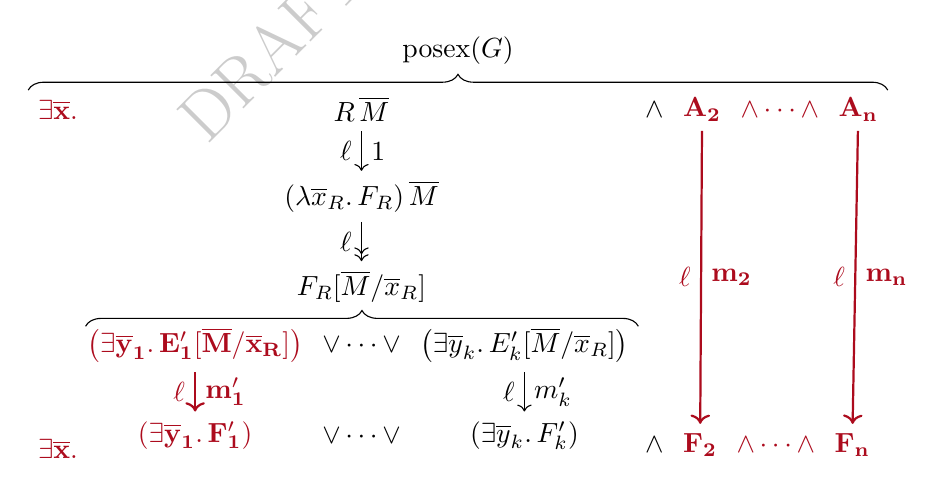
\begin{tikzpicture}
    \node (ex1) {$\color{oxred}\mathbf{\exists\overline x\ldotp}$};
    \node [right=3cm of ex1] (a11) {$R\,\overline M$};
    \node [right=30mm of a11] (l11) {$\land$};
    \node [right=0cm of l11] (a12) {$\color{oxred}\mathbf{A_2}$};
    \node [right=0cm of a12] (l12) {$\color{oxred}\mathbf{\land\cdots\land}$};
    \node [right=0cm of l12] (a1n) {$\color{oxred}\mathbf{A_n}$};

    \node [below=5mm of a11] (a21) {$(\lambda\overline x_R\ldotp F_R)\,\overline M$};
    \node [below=5mm of a21] (a31) {$F_R[\overline M/\overline x_R]$};
    \node [below=2mm of a31] (o41) {$\lor\cdots\lor$};
    \node [left=0cm of o41] (b41) {$\color{oxred}\mathbf{\left(\exists\overline y_1\ldotp E'_1[\overline M/\overline x_R]\right)}$};
    \node [right=0cm of o41] (b4k) {$\left(\exists\overline y_k\ldotp E'_k[\overline M/\overline x_R]\right)$};
    
    \node [below=7mm of o41] (o51) {$\lor\cdots\lor$};
    \node [below=5mm of b41] (b51) {$\color{oxred}\color{oxred}\mathbf{\left(\exists\overline y_1\ldotp F'_1\right)}$};
    \node [below=5mm of b4k] (b5k) {$\left(\exists\overline y_k\ldotp F'_k\right)$};

        
    \node [below=38.2mm of ex1] (ex5) {$\color{oxred}\mathbf{\exists\overline x\ldotp}$};

    \node [below=38.2mm of l11] (l51) {$\land$};
    \node [right=0cm of l51] (a52) {$\color{oxred}\mathbf{F_2}$};
    \node [right=0cm of a52] (l52) {$\color{oxred}\mathbf{\land\cdots\land}$};
    \node [right=0cm of l52] (a5n) {$\color{oxred}\mathbf{F_n}$};


    \draw [decorate, decoration={brace, amplitude=2mm}] (b41.north -| b41.west) +(1mm,-1mm) coordinate (a) -- (a -| b4k.east)+(-10mm,-10mm) node [midway,above=2mm, right=-11mm] {};
    
    \draw [decorate, decoration={brace, amplitude=2mm}] (ex1.north -| ex1.west) coordinate (a) -- (a -| a1n.east)+(-10mm,-10mm) node [midway,above=2mm] {$\posex(G)$};
    
    \path[->] (a11) edge [] node[left]{$\ell$} node[right]{$1$} (a21)
    (b4k) edge [] node[left]{$\ell$} node[right]{$m'_k$} (b5k);

    \path[->,thick] (b41) edge [color=oxred] node[left]{$\color{oxred}\mathbf{\ell}$} node[right]{$\color{oxred}\mathbf{m'_1}$} (b51)
    (a12) edge [color=oxred] node[left]{$\color{oxred}\mathbf{\ell}$} node[right]{$\color{oxred}\mathbf{m_2}$} (a52)
    (a1n) edge [color=oxred] node[left]{$\color{oxred}\mathbf{\ell}$} node[right]{$\color{oxred}\mathbf{m_n}$} (a5n);


    \path[->>] (a21) edge [] node[left]{$\ell$}  (a31);

  \end{tikzpicture}

  \caption{\label{fig:} Overview of\ \itemref{it:proofcase2} of the proof of \cref{lem:mudec}. The ingredients for $G'$,$F'$ and $m'$ are highlighted in bold and red for the case $\alpha[\overline y_1\mapsto\overline r]\force F'_1$.}
  \end{figure}
\begin{proof}
  Let $G\in S$ be goal clause, $F$ be a (closed) positive existential formula and let $m=\mu(G)>0$ be such that $\posex(G)\lred m F$ and $\force F$.
  Without loss of generality we can assume that
  \begin{align}
    \label{eq:varsdisjoint}
    \free(G)\cap\free(C)&=\emptyset& \text{for all } C\in S.
  \end{align}
  (Otherwise, rename all variables occurring in $G$ to obtain $\widetilde G$ satisfying \cref{eq:varsdisjoint} and clearly, by definition of $\Res$, $S\cup\{\widetilde G\}\Res S\cup\{\widetilde G,G'\}$ implies $S\Res S\cup\{G'\}$.)

  Furthermore, suppose that $G=\neg A_1\lor\cdots\lor\neg A_n$ and $\posex(G)=\exists\overline x\ldotp\bigland_{i=1}^n A_i$.
  By the Inversion \cref{lem:linversion}, there exist $F_1,\ldots,F_n$ and $m_1,\ldots,m_n$ such that $F=\exists\overline x\ldotp\bigland_{i=1}^n F_i$, $m=\sum_{i=1}^n m_i$ and $A_j\lred{m_j}F_j$ for each $1\leq j\leq m$. 
  Note that due to $\force F$ there exists a valuation $\alpha$ such that $\alpha\force F_j$ for each $1\leq j\leq n$.

  We can assume without loss of generality that $m_1>0$. By \cref{lem:lredassoc}, there exists $E$ such that $A_1\lred{1}E\lred{m_1-1}F_1$. Since $A_1$ is an atom there are exactly two cases:
  \begin{thmlist}
  \item $A_1=(\lambda y\ldotp L)M\,\overline N$ and $E=L[M/y]\overline N$ or
  \item\label{it:proofcase2} $A_1=R\,\overline M$ and $E=(\lambda\overline x_R\ldotp F_R)\overline M$.
  \end{thmlist}
  The first case is easy because for $G'=\neg L[M/y]\overline N\lor\biglor_{i=2}^n\neg A_i$, $S\cup\{G\}\Res S\cup\{G,G'\}$ and $\posex(G')=\exists\overline x\ldotp L[M/y]\overline N\land\bigland_{i=2}^n A_i$.
    
  In the second case, note that $\lred{1}$ is functional on applied $\lambda$-abstractions (by the Inversion \cref{lem:linversion}). Hence, we can assume that
    \begin{align*}
      (\lambda\overline x_R\ldotp F_R)\overline M\lredrt F_R[\overline M/\overline x_R]\lred{m^*_1}F_1,
    \end{align*}
    where $m^*_1\leq m_1-1$ for otherwise $\alpha\force F_1$ would clearly not hold.

    $F_R$ has the form $\posex(G_{R,1},\overline x_R)\lor\cdots\lor\posex(G_{R,k},\overline x_R)$, where each $G_{R,j}$ is a goal clause and $G_{R,j}\lor R\,\overline x_R\in S$. Let $\overline y_1,\ldots,\overline y_k$ and $E'_1,\ldots,E'_k$ be such that for each $j$, $\posex(G_{R,j},\overline x_R)=\exists\overline y_j\ldotp E_j'$. Note that by \cref{eq:varsdisjoint}, $\posex(G_R,\overline x_R)[\overline M/\overline x_R]=\exists\overline y_j\ldotp E'_j[\overline M/\overline x_R]$ for each $j$ and by the Inversion \cref{lem:linversion}, there exist $F_1',\ldots,F'_k$ and $m'_1,\ldots,m'_k$ such that $F_1=\bigvee_{j=1}^k(\exists\overline y_j\ldotp F_j')$, $E'_j[\overline M/\overline x_R]\lred{m_j'}F'_j$ and $m'_j\leq m_1^*$ for each $j$. 

Next, because of $\alpha\force F_1$ there exists $1\leq j\leq k$ and $\overline r\in\sinti\Hf{\Delta(\overline y_j)}$ satisfying $\alpha[\overline y_j\mapsto\overline r]\force F'_j$.
Furthermore, because of \cref{eq:varsdisjoint,lem:nonewfree,lem:vartrianglemodels}, $\alpha[\overline y_j\mapsto\overline r]\force F_i$ for all $2\leq i\leq n$. Therefore,
\begin{align}
  \label{eq:compalphamodels}\alpha[\overline y_j\mapsto\overline r]\force F'_j\land\bigwedge_{i=2}^n F_i.
\end{align}

Clearly, it holds that
\begin{align}
  \label{eq:compmakeres}S\cup\{G\}\Res S\cup\left\{G,G_{R,j}[\overline M/\overline x_R]\lor\biglor_{i=2}^n\neg A_i\right\},\\
  \label{eq:complred}E_j'[\overline M/\overline x_R]\land\bigland_{i=2}^n A_2\lred{m'_j+\sum_{i=2}^n m_i}F_j'\land\bigland_{i=2}^n F_i
\end{align}
and $\free(G')\subseteq\overline x\cup\overline y$. Let $\overline x'\subseteq\overline x$ and $\overline y'\subseteq\overline y$ be such that $\free(G')=\overline x'\cup\overline y'$. Hence, $\posex(G')=\exists\overline x',\overline y'\ldotp E_j'[\overline M/\overline x_R]\land\bigland_{i=2}^n A_2$.
We define
\begin{align*}
  G'&=G_{R,j}[\overline M/\overline x_R]\lor\biglor_{i=2}^n\neg A_i&F'&=\exists\overline x',\overline y'\ldotp E_j\land\bigland_{n=2}^n F_i&m'&=m'_j+\sum_{i=2}^n m_i.
\end{align*}
By \cref{eq:compalphamodels,eq:compmakeres,eq:complred}, it holds that
\begin{enumerate*}
\item $S\Res S\cup\{G'\}$,
\item $\posex(G')\lred{m'}F'$,
\item $\force F'$ and
\item $m'\leq m_1^*+\sum_{i=2}^n m_i<\sum_{i=1}^n m_i=m$.
\end{enumerate*}
Consequently, also $\mu(S\cup\{G'\})<\mu(S)$
\end{proof}

By the definition of $\alpha\force F$, it is very easy to refute sets of HoCHCs with measure 0. Therefore, we finally get:
\completeness*
\begin{proof}
  By \cref{lem:nfdefinite,lem:modp}, $\As^\Hf_P\models D$ for all definite clauses $D\in S$. Since $S$ is $(\As,\Hf)$-unsatisfiable there exists a goal clause $G\in S$ satisfying $\As^\Hf_P\not\models G$. By \cref{thm:contmain} there exists $n\in\omega$ such that $\As^\Hf_n\not\models G$. Let $F_n$ be such that $\posex(G)\pred^n F_n$. By \cref{lem:parallelcorr}, $\As^\Hf_0\models F_n$. Let $F_n'$ be the $\beta$-normal form of $F_n$. By \cref{lem:parallelbu,cor:sthi,lem:sdecompose} there exists $F'$ such that $\posex(G)\lredrt F'$ and $\force F'$. Consequently, $\mu(S)<\omega$. By \cref{lem:mudec} there exists $S'\supseteq S$ satisfying $S\Res^* S'$ and $\mu(S')=0$. 

  Hence, there exists $G\in S'$ such that $\posex(G)\lred{0} F'$ and $\force\posex(F')$. Besides, by \cref{lem:lred0}, $F'=\posex(G)$ and therefore $G$ has the form $G'\lor\neg\phi_1\lor\cdots\lor\neg\phi_n$, where $G'$ is simple and the $\phi_i$ are first-order such that there exists a valuation $\alpha$ satisfying $\As,\alpha\models\phi_1\land\cdots\land\phi_n$. Therefore, the rule Constraint Refutation is applicable to $G$ and hence, $S\Res^* S'\Res\{\bot\}\cup S'$.
\end{proof}

\chapter{Ramifications}
\label{ch:applications}
\label{CH:APPLICATIONS}
In this chapter, we apply the results of the previous chapter to obtain some interesting corollaries. In \cref{sec:equiv}, we prove that the satisfiability of higher-order constrained Horn clauses is independent of the choice of a Henkin frame. In particular, this re-proves the equivalence of standard, monotone and continuous semantics for HoCHCs.

\cref{sec:elimnest} demonstrates that every program can indeed be transformed into our normal form and that $\lambda$-abstractions can be eliminated.

These insights are used in \cref{sec:peuf}, where we relate our efforts to work on higher-order logic programming and show that we can also deal with some background theories with an infinite number of models.

Finally, \cref{sec:appenc} describes a reduction of HoCHCs to first-order logic with background theories.
\cref{fig:summary-results} summarises some of the results of this chapter.


\begin{figure}
  \centering
  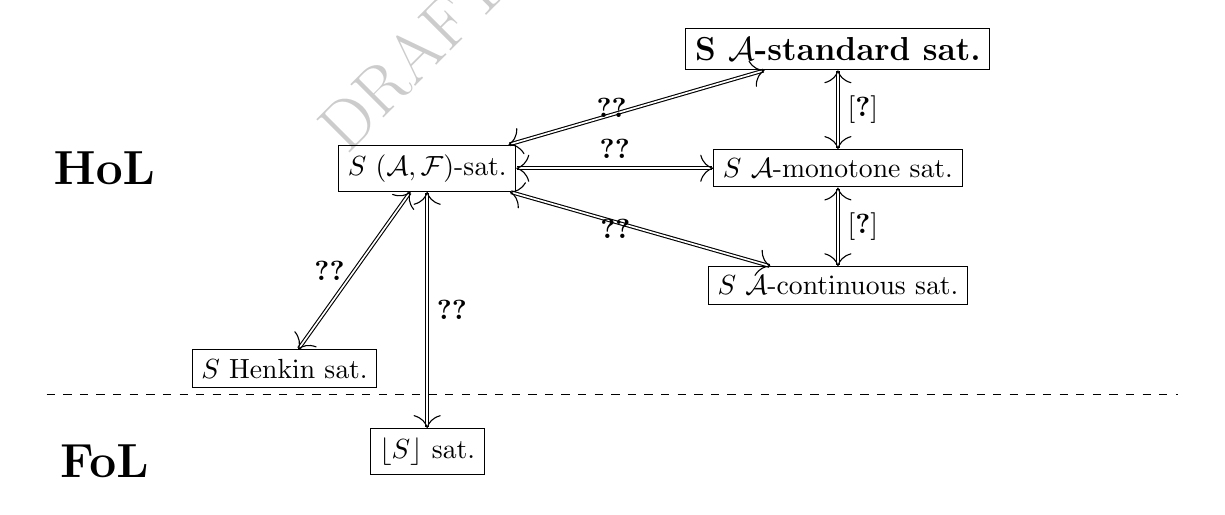
\begin{tikzpicture}
    \node[draw] (hs) {$S$ $(\As,\Hf)$-sat.};
    \node[draw,right=2.5cm of hs] (mon) {$S$ $\As$-monotone sat.};
    \node[draw,above=1cm of mon] (st) {\large{\textbf{$\mathbf{S}$ $\mathbf{\As}$-standard sat.}}};
    \node[draw,below=1cm of mon] (cont) {$S$ $\As$-continuous sat.};
    \node[draw,below left=2cm and -0.5cm of hs] (henkin) {$S$ Henkin sat.};

    \node[draw,below=3cm of hs] (fols) {$\lfloor S\rfloor$ sat.};

    \node[below left=2.45cm and 3.7cm of hs] (foo) {};
    \node[below right=2.45cm and 8.4cm of hs] (bar) {};

    \node[left=2.2cm of hs] (hol) {\LARGE{\textbf{HoL}}};
    \node[below=3.05cm of hol] (fol) {\LARGE{\textbf{FoL}}};

    \path[-]
    (foo) edge [dashed] (bar);
    
    \path[<->]
    (hs) edge [double] node [left] {\cref{sec:equiv}} (st)
    (hs) edge [double] node [above] {\cref{sec:equiv}} (mon)
    (hs) edge [double] node [left] {\cref{sec:equiv}} (cont)
    (hs) edge [double] node [left] {\cref{sec:equiv}} (henkin)
    (hs) edge [double] node [right] {\cref{sec:appenc}} (fols)
    (st) edge [double] node [right] {\cite{BOR18}} (mon)
    (mon) edge [double] node [right] {\cite{J18}} (cont);
    
    % \draw[double,<->] (st) -- node[above]{\cite{BOR18}} (mon);
  \end{tikzpicture}

  \caption{\label{fig:summary-results} Some results of \cref{ch:applications}.}
  \end{figure}

\section{Equivalence of Semantics}
\label{sec:equiv}
\label{SEC:EQUIV}
This section proves that the satisfiability problem for higher-order constrained Horn clauses coincides for all Henkin frames, which gives rise to an alternative proof of the equivalence of standard, monotone and continuous semantics for HoCHCs \cite{BOR18,J18}.
\begin{theorem}
  \label{thm:equivframes}
  Let $S$ be a set of HoCHCs and let $\Hf$ and $\Hf'$ be Henkin frames
  such that $S$ is $(\As,\Hf)$-unsatisfiable. Then $S$ is also $(\As,\Hf')$-unsatisfiable.
\end{theorem}
\begin{proof}
  By the Completeness \cref{thm:completeness}, $S\Res^*\{\bot\}\cup S'$ for some $S'$ and by soundness of resolution (\cref{prop:soundness}), $S$ is $(\As,\Hf')$-unsatisfiable.
  % Assume towards contradiction that there exists a $(\Sigma',\Hf)$-expansion $\Bs$ of $\As$ satisfying $\Bs\models_\Hf S$ and assume that $S$ is $(\As,\Hf')$-unsatisfiable. Then by \cref{thm:completeness}, $S\Res^*\{\bot\}\cup S'$ for some $S'$ and by \cref{prop:soundness}, $\Bs\models\bot$, which is clearly a contradiction.
\end{proof}


Next, note that $\crel$ and $\prel$ coincide for the continuous frame. The straightforward proof can be found in \cref{app:applications}.
\begin{restatable}{lemma}{cprel}
  \label{cl:cprel}
  $\crel^\Cf\;=\;\prel^\Cf$.
\end{restatable}

The proof of the following makes use of \cref{cl:cprel} and differs from the proof of \cref{lem:contmain} only in the case of $\lambda$-abstractions. The details can be found in \cref{app:applications}.
\begin{restatable}{lemma}{conhenkin}
  \label{lem:conhenkin}
  Let $\Sigma$ be a signature, $\Delta$ be a type environment and $\Bs$ be a $(\Sigma,\Cf)$-structure. 
  
  Then for any positive existential term $M$, $(\Delta,\Cf)$-valuation $\alpha$ and $\Ad'\in\dir(\alpha)$,
  \begin{thmlist}
  \item\label{it:conhenkin1} if $M$ is a $\lambda$-abstraction then $\Bs^\Cf\langle M\rangle(\alpha)=\sinti{\Bs^\Cf}{M}(\alpha)$ and
  \item\label{it:conhenkin2} $\sinti{\Bs^\Cf} M(\bigsqcup\Ad)\crel\bigsqcup\{\sinti{\Bs^\Cf} M(\alpha)\mid\alpha\in\Ad\}$.
  \end{thmlist}
\end{restatable}
Similarly, we get the following for the monotone frame
\begin{lemma}
  \label{lem:monhenkin}
  \begin{thmlist}
  \item $\mrel^\Mf=\prel^\Mf$;
  \item If $\Sigma$ is a signature, $\Delta$ is a type environment, $\As$ is a $(\Sigma,\Mf)$-structure, $\alpha$ is a $(\Delta,\Mf)$-valuation, $\lambda x\ldotp M$ is a positive existential $\Sigma$-term then
    \begin{align*}
      \As^\Mf\langle M\rangle(\alpha)=\sinti{\As^\Mf}{M}(\alpha).
    \end{align*}
  \end{thmlist}
\end{lemma}
\cref{lem:monhenkin,lem:conhenkin} immediately imply:
\begin{proposition}
  \label{prop:Henkin}
  $\Sf$, $\Mf$ and $\Cf$ are Henkin frames.
\end{proposition}
Finally, by \cref{thm:equivframes,prop:Henkin}, we get the main result of this section:
\begin{theorem}[Equivalence of Semantics]
  \label{thm:equivsem}
  Let $S$ be a set of HoCHCs. Then the following are equivalent:
  \begin{thmlist}
  \item $S$ is $\As$-standard-satisfiable,
  \item $S$ is $\As$-Henkin-satisfiable,
  \item $S$ is $\As$-monotone-satisfiable,
  \item $S$ is $\As$-continuous-satisfiable,
  \item $S$ is $(\As,\Hf)$-satisfiable, where $\Hf$ is a Henkin frame.
  \end{thmlist}
\end{theorem}

We call a set of $S$ of HoCHCs \emph{$\As$-satisfiable} if it satisfies any of the conditions of the preceding theorem.

\section{Elimination of Nested Terms}
\label{sec:elimnest}
\label{SEC:ELIMNEST}
In this section, we show how to eliminate terms which are nested to a certain extend. We use this insight for a normal form transformation and to remove $\lambda$-abstractions.

 Consider for example the rather peculiar formula $R\,\lor$, where $R\from(o\to o\to o)\to o$. In  full higher-order relational logic we could introduce a new symbol $U\from o\to o\to o$, add the ``definition'' $U\,x\,y\leftrightarrow (x\lor y)$ and replace $R\,\lor$ with $R\,U$. These definitions cannot be transformed into HoCHCs because the ``$\rightarrow$''-direction $\neg U\,x\,y\lor (x\lor y)$ clearly does not correspond to a HoCHC. Rather, we use ideas inspired by \cite{PG86} to show that adding the unproblematic direction $\neg x\lor U\,x\,y$ and $\neg y\lor U\,x\,y$ is sufficient. However, we have to greatly generalise their approach, which is for formulas of first-order logic, to arbitrary relational, positive existential higher-order terms.

Let $M$ be a positive existential $\Sigma'$-term with free variables $\overline x$ such that $\Delta\vdash M\from\overline\tau\to o$, let $\widetilde P[-]$ be a set of terms with a hole of type $\overline\tau\to o$ such that $P[M]$ is a program and let $\widetilde F[-]$ be a term with a hole of type $\overline\tau\to o$ such that $F[M]$ is a positive existential formula.

Assume that $\Delta(\overline x)=\overline\tau'$ and let $\overline y$ be distinct variables (different from $\overline x$) satisfying $\Delta(\overline y)=\overline\tau$. We define a signature $\Sigma''=\Sigma'\cup\{R_M\from\overline\tau'\to\overline\tau\to o\}$ and
\begin{align*}
  P&=\widetilde P[M]&F&=\widetilde F[M]\\
  P'&=\widetilde P[R_M\,\overline x]\cup\{\neg M\,\overline y\lor R_M\,\overline x\,\overline y\}&F'&=\widetilde F[R_M\,\overline x].
\end{align*}
These are clearly programs and positive existential formulas, respectively.
In the following we prove that $(P,F)$ and $(P',F')$ are in fact $(\As,\Hf)$-equivalent for every Henkin frame $\Hf$. First, note that the proof of \cref{lem:termmon} can be adapted in a straightforward manner to obtain:
\begin{lemma}
  \label{lem:termmonhole}
  Let $\Bs$ be a $\Sigma'$- and $\Bs'$ be a $\Sigma''$-structure, let $M[-]$ be a $\Sigma'$-term with a hole of type $\tau$, let $N$ be a $\Sigma'$ and $N'$ be a $\Sigma''$-formula satisfying
  \begin{thmlist}
  \item $M[N]$ is a positive existential formula,
  \item $\Delta\vdash N\from\tau$ and $\Delta\vdash N'\from\tau$,
  \item for all $R\in\Sigma'\setminus\Sigma$, $R^\Bs\mrel R^{\Bs'}$
  \item for all $(\Delta,\Hf)$-valuations $\alpha\mrel\alpha'$, $\hinti\Bs N(\alpha)\mrel\hinti{\Bs'}{N'}(\alpha')$.
  \end{thmlist}
  Then for all $(\Delta,\Hf)$-valuations $\alpha\mrel\alpha'$, $\hinti\Bs{M[N]}(\alpha)\mrel\hinti{\Bs'}{M[N']}(\alpha')$.
\end{lemma}
In the following lemma we prove that although $\As^\Hf_{P',n}$ ``grows slower'' (with increasing $n\in\omega$) than $\As^\Hf_{P,n}$, $\As^\Hf_{P',2n+1}$ still roughly ``catches up'' with $\As^\Hf_{P,n}$.
\begin{restatable}{lemma}{elimrel}
  \label{lem:elimrel}
  For every $n\in\omega$, 
  \begin{thmlist}
  \item $R^{\As^\Hf_{P,n}}\mrel R^{\As^\Hf_{P',2n}}$ for $R\in\Sigma'\setminus\Sigma$,
  \item $R^{\As^\Hf_{P,n}}\mrel R^{\As^\Hf_{P',2n+1}}$ for $R\in\Sigma'\setminus\Sigma$ and
  \item $\sinti{\As^\Hf_{P,n}}{\lambda\overline x\ldotp M}(\top_\Delta^\Hf)\mrel R_M^{\As^\Hf_{P',2n+1}}$.
  \end{thmlist}
\end{restatable}
It is proven in detail in \cref{app:elimnest}. As a consequence we get:
\begin{proposition}
  \label{prop:elimnested}
  Let $\Hf$ be a Henkin frame.
  Then $(P,F)$ is $(\As,\Hf)$-equivalent to $(P',F')$.
\end{proposition}
\begin{proof}
  \begin{itemize}
  \item First, suppose that there exists a $(\Sigma',\Hf)$-expansion $\Bs$ of $\As$ satisfying $\Bs\models_\Hf P$ and $\Bs\not\models F$. We define a $(\Sigma'',\Hf)$-expansion $\Bs'$ of $\As$ by setting $R^{\Bs'}=R^\Bs$ for $R\in\Sigma'\setminus\Sigma$ and $R_M^{\Bs'}=\hinti\Bs{\lambda\overline x,\overline y\ldotp M\,\overline y}(\top_{\Sigma'}^\Hf)$. By definition, $\Bs'\models_\Hf\neg M\,\overline y\lor R_M\,\overline x\,\overline y$. Furthermore for every positive existential $\Sigma'$-formula $E$ and $(\Delta,\Hf)$-valuation $\alpha$, by \cref{lem:contextequal}, $\sinti\Bs{E[M]}(\alpha)=\sinti{\Bs'}{E[R_M\,\overline x]}(\alpha)$.
    Consequently, $\Bs'\models_\Hf P'$ and $\Bs'\not\models F'$.
  \item Conversely, suppose that there exists a $(\Sigma'',\Hf)$-expansion $\Bs'$ of $\As$ satisfying $\Bs'\models_\Hf P'$ and $\Bs'\not\models F'$. % By \cref{lem:canmod2}, $\As^\Hf_{P'}\mrel\Bs'$ and therefore by \cref{lem:termmon}, $\As^\Hf_{P'}\not\models F$.
    Assume towards contradiction that $\As_P^\Hf\models F$. Then, by \cref{thm:contmain}, $\As^\Hf_{P,n}\models F$  for some $n\in\omega$.
    By \cref{lem:elimrel,lem:termmonhole}, $\As^\Hf_{P',2(n+1)}\models F'$ and therefore, by \cref{lem:termmon,it:allordsmaller}, $\As^\Hf_{P'}\models F'$. Note that by \cref{lem:canmod2}, $\As^\Hf_{P'}\mrel\Bs'$ and therefore, by \cref{lem:termmon}, $\Bs'\models F'$, which is clearly a contradiction.

    Consequently, $\As^\Hf_P\not\models F$ and by \cref{lem:modp}, $\As^\Hf_P\models_\Hf P$.\qedhere
  \end{itemize}
\end{proof}

\subsection{Normal Form Transformation}
\label{sec:normalform}
In this subsection, we use the insights just gained to show how to obtain a HoCHC in normal form which is equivalent to a given HoCHP. This closes the gap in the translation of HoCHPs to HoCHCs from \cref{sec:nftrans}.

There are two important tasks to accomplish:
\begin{enumerate*}
\item eliminating terms of the form $R\,\overline M$, $x\,\overline M$ or $(\lambda x\ldotp N)\,\overline M$, where $\overline M$ or $N$ contain logical symbols,
\item establishing the logical structure ``$\bigvee\exists\bigwedge$''.
\end{enumerate*}

To achieve the first goal we make more precise which terms we need to eliminate.
\begin{definition}
  \begin{thmlist}
  \item A term $c\,\overline M$ \defia{occurs impure}{occur impure} in a formula $N_1\cdots N_n$ if
    \begin{enumerate*}
    \item $c\,\overline M$ is a subterm of $N_1\cdots N_n$,
    \item $c$ is a logical symbol and
    \item $N_1\in\Sigma'$, $N_1$ is a variable or $N_1$ is a $\lambda$-abstraction.
    \end{enumerate*}
  \item A term $M$ \emph{occurs impure} in $(P,F)$ if there exists a term $N$ such that $M$ occurs impure in $N$ and $N$ is a subterm of a term in $P\cup\{F\}$.
  \item $(P,F)$ is \defis{pure}{constrained Horn problem in program form} if there are is no term which occurs impure in $(P,F)$.
  \end{thmlist}
\end{definition}
\begin{example}
  Consider $\exists(\lambda x\ldotp R\,(x=x)\lor R\,(x\leq x\land x\geq x))$. $(x\leq x\land x\geq x)$, which is an abbreviation for $\land\,(x\leq x)\,(x\geq x)$, occurs impure in $R\,(x\leq x\land x\geq x)$. $R\,(x=x)\lor R\,(x\leq x\land x\geq x)$ does not occur impure in $\lambda x\ldotp R\,(x=x)\lor R\,(x\leq x\land x\geq x)$ because the latter is no formula.
\end{example}
Clearly, there is no term which occurs impure in an atom.

\begin{proposition}
  \label{lem:nfpure}
  Let $\Hf$ be a Henkin frame and $(P,F)$ be a HoCHP.

  Then there exists a $(\As,\Hf)$-equivalent HoCHP which is pure.
\end{proposition}
\begin{proof}
  We prove the lemma by induction on the number $m$ of distinct terms $M$ which occur impure in $(P,F)$. If $m=0$ then $(P,F)$ is clearly pure. 

  Otherwise there exists a term $M$ which 
  \begin{enumerate*}
  \item occurs impure in $(P,F)$ and
  \item\label{lem:eimimpure2} is not a subterm of another term which occurs impure in $(P,F)$.
  \end{enumerate*}
  Suppose $\Delta\vdash M\from\rho$. By \cref{lem:contextex} there are (sets of) contexts with a $\rho$-hole $\widetilde P[-]$ and $\widetilde F[-]$ such that $\widetilde P[M]=P$, $\widetilde F[M]=F$ and $M$ occurs neither in $\widetilde P[-]$ nor in $\widetilde F[-]$. Let $P'=\widetilde P[R_M\,\overline x]\cup\{\neg M\,\overline y\lor R_M\,\overline x\,\overline y\}$ and $F'=\widetilde F[R_M\,\overline x]$. $(P,F)$ and $(P',F')$ are $(\As,\Hf)$-equivalent by \cref{prop:elimnested}. 

Note that $M$ does not occur impure in $(P',F')$. Furthermore, by \cref{lem:eimimpure2}, each term which contains impure in $(P',F')$ also occurs impure in $(P,F)$. Hence, the number of distinct terms which occur impure in $(P',F')$ is strictly smaller than $m$. Consequently, by the inductive hypothesis, $(P',F')$ is $(\As,\Hf)$-equivalent to some pure $(P'',F'')$.
\end{proof}

Therefore, we can assume that $(P,F)$ is pure. Note that by \cref{lem:etaequal} we can furthermore assume that for all occurrences of a term $\exists M$ in $P\cup\{F\}$, $M$ is a $\lambda$-abstraction. Hence, each positive existential formula occurring in $P\cup\{F\}$ has the form
\begin{align*}
  F_l::=A\mid F_l\land F_l\mid F_l\lor F_l\mid\exists x\ldotp F_l,
\end{align*}
where $A$ is an atom and $x$ is a variable. Clearly, we can transform each such positive existential formula into normal form by exploiting the distributivity law and pushing the existential quantifier inside or outside exactly as for the DNF-transformation (or dually CNF-transformation) for first-order logic (see e.g.\ \cite{NW01}). 
Hence, we get:
\begin{theorem}
  Let $\Hf$ be a Henkin frame and $(P,F)$ be a HoCHP.

  Then there exists a $(\As,\Hf)$-equivalent HoCHP in normal form. 
\end{theorem}
\begin{example}
  Consider the program $\{\neg (\exists x\ldotp (R\,\lor)\land (x\lor(\lambda y\ldotp y\land y)x))\lor R\,z\}$ and the positive existential formula $\exists x\ldotp x$. The elimination of impure terms results in the program
  \begin{align*}
    \{\neg (\exists x\ldotp R\,R_\lor\land (x\lor(\lambda y\ldotp R_{y\land y}\,y)x))&\lor R\,z,\\
    \neg (x\lor y)&\lor R_\lor\,x\,y\\
    \neg (y\land y)&\lor R_{y\land y}\,y\}.
  \end{align*}
  After establishing the required logical structure we get:
    \begin{align*}
      \{\neg ((\exists x\ldotp R\,R_\lor\land x)\lor(\exists x\ldotp R\,R_\lor\land(\lambda y\ldotp R_{y\land y}\,y)x))&\lor R\,z,\\
      \neg (x\lor y)&\lor R_\lor\,x\,y\\
      \neg (y\land y)&\lor R_{y\land y}\,y\}.
  \end{align*}
\end{example}
Note that using distributivity exhaustively may result in an exponential blow-up in the size of the HoCHP. To counteract this, we could introduce ``renamings'' exactly as in first-order logic, exploiting the insights gained in the previous section. However, this is not the focus of the present work and the interested reader should refer to e.g.\ \cite{PG86} or \cite{NW01} for a good exposition.

\subsection{Elimination of $\lambda$-Abstractions}
Next, we show that for each set $S$ of HoCHCs there exists a set $S'$ of HoCHCs which does not contain $\lambda$-abstractions and which is $(\As,\Hf)$-satisfiable if and only if $S$ is $(\As,\Hf)$-satisfiable. We use the results from \cref{sec:normalform}, which are stated for HoCHPs. Since HoCHPs may contain $\lambda$-abstractions (implicitly) below existential quantifiers, we first have to make precise when a HoCHC ``essentially'' does not contain $\lambda$-abstractions:
\begin{definition}
  \begin{thmlist}
  \item A positive existential term $M$ is \defias{$\lambda$-free}{$\lambda$-free positive existential term}{term} it has the form
    \begin{align*}
      M_\lambda::=x\mid c\mid\land\mid\lor\mid \exists\tau(\lambda x\ldotp M_\lambda)\mid M_\lambda M_\lambda
    \end{align*}
  \item A HoCHP $(P,F)$ is \defis{$\lambda$-free}{constrained Horn problem in program form} if all positive existential subformulas of formulas in $P\cup\{F\}$ are $\lambda$-free.
  \end{thmlist}
\end{definition}
Analogously to \cref{lem:nfpure} we get (the details are presented in \cref{app:elimnest}):
\begin{restatable}{proposition}{elimlambda}
  \label{lem:elimlambda}
  Let $\Hf$ be a Henkin frame and $(P,F)$ be a HoCHP in normal form.

  Then there exists a $\lambda$-free HoCHP in normal form which is $(\As,\Hf)$-equivalent to $(P,F)$.
\end{restatable}

Hence, using the translations from HoCHCs to HoCHP in normal form (\cref{lem:assocprgmnew}), the elimination of $\lambda$-abstractions (\cref{lem:elimlambda}) and the translation back to HoCHCs (\cref{cor:transprgmcl}) we get:
\begin{theorem}
  \label{thm:ellambdahochc}
  Let $\Hf$ be a Henkin frame and $S$ be a set of HoCHCs. 

  Then there exists a set of HoCHCs which does not contain $\lambda$-abstractions and which is $(\As,\Hf)$-satisfiable if and only if $S$ is $(\As,\Hf)$-satisfiable.
\end{theorem}

Note that in the proof of \cref{thm:ellambdahochc} we eliminate more $\lambda$-abstractions than strictly necessary, some of which we have to reintroduce to obtain a normal form:
\begin{example}
  Consider an arbitrary program $P$ and the positive existential formula $R\,(\lambda x\ldotp x)\lor\exists x\ldotp x$, which is an abbreviation for $R\,(\lambda x\ldotp x)\lor\exists(\lambda x\ldotp x)$. The proof of \cref{lem:elimlambda} constructs a HoCHP $(P'\cup\{\neg x\lor R_{\lambda x\ldotp x}\,x\},R\,R_{\lambda x\ldotp x}\lor\exists R_{\lambda x\ldotp x})$. However, there is no need to eliminate the $\lambda$-abstraction in $\exists(\lambda x\ldotp x)$ and we could have taken $(P'\cup\{\neg x\lor R_{\lambda x\ldotp x}\,x\},R\,R_{\lambda x\ldotp x}\lor\exists x\ldotp x))$, which is $\lambda$-free and in normal form, too.
\end{example}


\section{Resolution for the Theory of Positive Equality and Uninterpreted Functions}
\label{sec:peuf}
In this section, we show how to use our framework to solve the problem considered by \cite{CHRW13} (cf.\ the discussion in \cref{sec:discussion,sec:relworkrel}) with respect to arbitrary Henkin frames. In \cref{sec:normalform}, we bridged the difference in terms of syntax. Therefore, it only remains to demonstrate how we can determine satisfiability of unconstrained Horn clauses.

Formally, let $\Sigma'$ be a signature containing the equality symbol $\approx\from\iota\to\iota\to o$. Then, there exists a (unique) $\Sigma\subseteq\Sigma'$ such that $\approx\;\in\Sigma$, $\Sigma\setminus\{\approx\}$ contains only symbols of type $\iota^n\to\iota$ and $\Sigma'\setminus\Sigma$ is purely relational. Furthermore, let $\Hd$ be a non-empty class of Henkin frames (e.g. $\{\Cf_D\mid D\text{ a set}\}$ or $\{\Hf\mid\Hf\text{ is a Henkin frame}\}$).
\begin{definition}
  A set $S$ of $(\Sigma,\Sigma')$-HoCHC is \emph{$\Hd$-satisfiable} if there exists $\Hf\in\Hd$ and a $(\Sigma',\Hf)$-structure $\Bs$ such that $\Bs\models_\Hf S$ and $\approx^\Bs(n)(m)=1$ if and only if $n=m$.
\end{definition}

\begin{proposition}
  \label{prop:Herbrand}
  Let $S$ be a set of HoCHCs. 
  $S$ is $\Hd$-satisfiable if and only if there exists some $\Hf\in\Hd$ such that $S$ is $(\As_{\Her},\Hf)$-satisfiable.
\end{proposition}
\begin{proof}
  If $S$ is $(\As_{\Her},\Hf)$-satisfiable for some $\Hf\in\Hd$ then $S$ is clearly $\Hd$-satisfiable.

Conversely, suppose $S$ is $\Hd$-satisfiable. Then, there exists $\Hf\in\Hd$ and a $(\Sigma',\Hf)$-structure $\Bs$ such that $\Bs\models_\Hf S$ and $\approx^\Bs(n)(m)=1$ if and only if $n=m$. Assume towards contradiction that $S$ is not $(\As_{\Her},\Hf)$-satisfiable. Then by the Completeness \cref{thm:completeness} there exists $S'$ and $G\lor\neg (M_1\approx N_1)\lor\cdots\lor\neg (M_n\approx N_n)$ in $S'$ such that $\bot\not\in S'$, $S\Res^*S'$, $G$ is simple and there exists a valuation $\alpha$ such that $\As_{\Her},\alpha\models M_1\approx N_1\land\cdots\land M_n\approx N_n$.

Let $\alpha'(x)=\hinti\Bs{\alpha(x)}(\top_\Delta^\Hf)$ (the valuation $\top_\Delta^\Hf$ is clearly not of importance).
Note that for each $\Sigma$-term $L$,
\begin{align*}
  \hinti\Bs{L}(\alpha')=\hinti\Bs{\sinti{\As_{\Her}}{L}(\alpha)}(\top_\Delta^\Hf).
\end{align*}

% Then,
% \begin{align*}
%   \hinti\Bs{M_i}(\alpha')&=\hinti\Bs{\sinti{\As_{\Her}^\Sf}{M_i}(\alpha)}(\top_\Delta^\Hf)&\hinti\Bs{N_i}(\alpha')&=\hinti\Bs{\sinti{\As_{\Her}^\Sf}{N_i}(\alpha)}(\top_\Delta^\Hf)
% \end{align*}
% for each $i$.
Therefore, $\Bs,\alpha'\models M_1\approx N_1\land\cdots\land M_n\approx N_n$. This constitutes a contradiction because due to \cref{prop:soundness,lem:ignoresimple}, $\Bs,\alpha'\models\neg (M_1\approx N_1)\lor\cdots\lor\neg (M_n\approx N_n)$. 
\end{proof}
Consequently, by the Equivalence of Semantics \cref{thm:equivsem}, it suffices to check whether $S$ is $(\As_{\Her},\Hf)$-satisfiable for a fixed $\Hf\in\Hd$ using the resolution proof system. Clearly, this gives rise to a semi-decision procedure because checking whether there exists a valuation such that $\As_{\Her},\alpha\models M_1\approx N_1\land\cdots\land M_n\approx N_n$ just amounts to the problem whether $(M_1,\ldots,M_n)$ and $(N_1,\ldots,N_n)$ are unifiable.


\section{Applicative Encoding}
\label{sec:appenc}
\label{SEC:APPENC}


Finally, we present a way to reduce the $\As$-satisfiability problem for HoCHCs to the satisfiability problem of first-order logic modulo a theory by using an applicative encoding in the spirit of e.g.\ \cite{BD83,K91,BKPU16}. We prove that this translation is sound and complete, and demonstrate that the target logic still admits refutationally complete proof systems.
As a consequence of \cref{thm:ellambdahochc}, we do not need to consider sets of HoCHCs containing $\lambda$-abstractions.


Clearly, the signature $\Sigma$ and the $\Sigma$-structure $\As$ can be regarded as a many-sorted signature and structure, respectively (with only one sort $\iota$).
Let $\lfloor\Sigma'\rfloor$ be the many-sorted first-order signature, which extends $\Sigma$ with
\begin{enumerate}[noitemsep]
\item the (foreground) sorts $\lfloor\rho\rfloor$ for relational $\rho$ (and we set $\lfloor\iota^n\to\iota\rfloor=\iota^n\to\iota$),
\item constants $c_R\from\lfloor\rho\rfloor$ for $R\from\rho\in\Sigma'\setminus\Sigma$ and $c_\rho\from\lfloor\rho\rfloor$ for relational types $\rho$,
\item a binary function symbol $\app_{\tau,\rho}\from\lfloor\tau\to\rho\rfloor\to\lfloor\tau\rfloor\to\lfloor\rho\rfloor$ for each relational type $\tau\to\rho$ and
\item a monadic relation symbol $H\from\lfloor o\rfloor\to o$.
\end{enumerate}
To enhance readability we frequently omit the subscript from $\app$ in what follows. The following observation is trivial:
\begin{lemma}
  \label{lem:suffcomp}
  $(\Sigma,\{\As\},\lfloor\Sigma'\rfloor)$ is a hierarchic specification and $\lfloor\Sigma'\rfloor$ does not contain a function symbol $f\from\lfloor\tau_1\rfloor\to\cdots\to\lfloor\tau_n\rfloor\to\iota$.
\end{lemma}
Let $\lfloor\Delta\rfloor$ be the type environment consisting of $x\from\lfloor\tau\rfloor$ whenever $x\from\tau\in\Delta$ and variables $x_{\tau_i}^{(i)}$ for relational $\tau_1\to\cdots\to\tau_n\to o$.
For a $\Sigma'$-term $M$ containing neither logical symbols nor $\lambda$-abstractions, we define $\lfloor M\rfloor$ by structural induction:
\begin{align*}
  \lfloor x\rfloor&=x,\\
  \lfloor R\rfloor&=c_R,&\text{if }R\in\Sigma'\setminus\Sigma,\\
  \lfloor c\,\overline N\rfloor&= c\,\overline N,&\text{if $c\in\Sigma$},\\
  \lfloor M\,\overline NN'\rfloor&=\app\,\lfloor M\,\overline N\rfloor\,\lfloor N'\rfloor,&\text{if $M\nin\Sigma$}.
\end{align*}
Note that because of \cref{rem:isimple}, for each $\Sigma'$-term $M$, $\lfloor M\rfloor$ is a $\lfloor\Sigma'\rfloor$-term, and $\Delta\vdash M\from\sigma$ if and only if $\lfloor\Delta\rfloor\vdash\lfloor M\rfloor\from\lfloor\sigma\rfloor$.
For higher-order constrained Horn clauses we define
\begin{align*}
  \lfloor\neg A_1\lor\cdots\lor\neg A_n\rfloor&=\neg\lfloor A_1\rfloor\lor\cdots\lor\neg\lfloor A_n\rfloor,\\
  \lfloor\neg A_1\lor\cdots\lor\neg A_n\lor R\,\overline x_R\rfloor&=\neg\lfloor A_1\rfloor\lor\cdots\lor\neg\lfloor A_n\rfloor\lor\lfloor R\,\overline x_R\rfloor.
\end{align*}

Furthermore, for relational $\rho=\tau_1\to\cdots\to\tau_n\to o$, we define
 \begin{align*}
   \Comp_\rho=H\, (\app\, (\cdots(\app\,(\app\,c_\rho\,x_{\tau_1}^{(1)})\,x_{\tau_2}^{(2)})\cdots )\,x_{\tau_n}^{(n)})
 \end{align*}
 and for a set $S$ of HoCHCs which does not contain $\lambda$-abstractions, let
 \begin{align*}
   \lfloor S\rfloor=\{\lfloor C\rfloor\mid C\in S\}\cup\{\Comp\rho\mid x\from\rho\in\Delta\text{ occurs in }S\}.
 \end{align*}
 Note that $\lfloor S\rfloor$ is a set of $\lfloor\Sigma'\rfloor$-Horn clauses.
 
 \begin{example}
   Consider again the set $S$ of HoCHCs from \cref{ex:HoCHC}. Applying the encoding $\lfloor S\rfloor$ to $S$ we get:
   \begin{align*}
     \lfloor D_1\rfloor&=\neg(z=x+y)\lor H\,(\app\, (\app\, (\app\,\Add\,x)\,y)\,z)\\
     \lfloor D_2\rfloor&=\neg(n\leq 0)\lor\neg(s=x)\lor H\,(\app\,(\app\, (\app\, (\app\,\Iter\,f)\,s)\,n)\,x)\\
     \lfloor D_3\rfloor&=\neg(n>0)\lor\neg H\,(\app\,(\app\, (\app\, (\app\,\Iter\,f)\,s)\,(n-1))\,y)\lor\neg H\,(\app\,(\app\,(\app\,f\,n)\,y)\,x)\\
     &\hspace{0.45cm}\lor H\,(\app\,(\app\, (\app\, (\app\,\Iter\,f)\,s)\,n)\,x)\\
     \lfloor G\rfloor&=\neg(n\geq 1)\lor\neg H\,(\app\,(\app\, (\app\, (\app\,\Iter\,\Add)\,n)\,n)\,x)\lor\neg(x\leq n+n)\\
     \Comp_{\iota^3\to o}&=H\,(\app\,(\app\,(\app c_{\iota^3\to o}\, x_1)\,x_2)\,x_3)
   \end{align*}
 \end{example}



 \begin{proposition}[Soundness of Encoding]
   \label{prop:folpreservesat}
   If $S$ is satisfiable then $\lfloor S\rfloor$ is satisfiable.
 \end{proposition}
 \begin{proof}
   First suppose $S$ is satisfiable. Then, there exists a $(\Sigma',\Sf)$-expansion $\Bs$ of $\As$ satisfying $\Bs\models_\Sf S$. We define a many-sorted first-order $\lfloor\Sigma\rfloor$-expansion $\lfloor\Bs\rfloor$ of $\As$ by % interpreting the background sort $\iota$ by $\dom(\As)$, all symbols from $\Sigma$ by the corresponding interpretation by $\As$ and by
   setting
   \begin{enumerate}[noitemsep]
   \item $\sinti{\lfloor\Bs\rfloor}{\lfloor\rho\rfloor}=\sinti\Hf\rho$ for relational $\rho$,
   \item $c_R^{\lfloor\Bs\rfloor}=R^\Bs$ for $R\in\Sigma'\setminus\Sigma$ and $c_\rho^{\lfloor\Bs\rfloor}=\top_\rho^\Sf$ for relational $\rho$,
   \item $\app_{\tau,\rho}(r)(s)=r(s)$ for relational $\tau\to\rho$, $r\in\sinti{\lfloor\Bs\rfloor}{\lfloor\tau\to\rho\rfloor}$ and $s\in\sinti{\lfloor\Bs\rfloor}{\lfloor\tau\rfloor}$,
   \item $H^{\lfloor\Bs\rfloor}(b)=b$ for $b\in\sinti{\lfloor\Bs\rfloor}{\lfloor o\rfloor}=\bool$.
   % \item $\app_{\tau\to\rho}^{\lfloor\Bs\rfloor}(r)(s)=r(s)$ for argument types and relational types $\rho$,
   % \item $c_R^{\lfloor\Bs\rfloor}=R^\Bs$ for $R\in\Sigma'\setminus\Sigma$ and $c_\rho^{\lfloor\Bs\rfloor}=\top_\rho^\Hf$ for relational types $\rho$.
   \end{enumerate}
   Clearly, $\lfloor\Bs\rfloor\models\Comp_\rho$ for each relational $\rho$. Furthermore, for each $\Sigma'$-term $M$, $(\Delta,H)$-valuation $\alpha$ and $\lfloor\Delta\rfloor$-valuation $\lfloor\alpha\rfloor$, $\hinti\Bs M(\alpha)=\sinti{\lfloor\Bs\rfloor}{\lfloor M\rfloor}(\lfloor\alpha\rfloor)$ if for all $x\in\dom(\Delta)$, $\alpha(x)=\lfloor\alpha\rfloor(x)$. Furthermore, each $C\in S$ only contains variables from $\Delta$. Consequently, due to $\Bs\models_\Sf S$, $\lfloor\Bs\rfloor\models\lfloor S\rfloor$.
 \end{proof}
 Next, we prove that the encoding is in fact also complete, i.e.\ if $S$ is unsatisfiable then also $\lfloor S\rfloor$ is unsatisfiable. We proceed by introducing a proof system for the hierarchic specification (similar to the one in \cite{BGW94}) and showing that it can simulate refutations of $S$ on $\lfloor S\rfloor$.

 \inferbin{FO-Resolution}{\neg H\,M\lor G}{G'\lor H\,M'}{(G\lor G')\theta}{provided $G$ is a unifier of $M$ and $M'$.}


\medskip

\inferun{FO-Constraint Refutation}{\neg\phi_1\lor\cdots\lor\neg\phi_n}{\bot}{provided each $\phi_i$ is a $\Sigma$-term and there exists a valuation $\alpha$ such that $\As,\alpha\models\phi_1\land\cdots\land\phi_n$.}
\bigskip

Similarly as for $\Res$, we write $S\FORes S\cup\{C\}$ if $C$ can be derived from clauses in $S$ using any of the above two rules and $\FORes^*$ for the reflexive, transitive closure of $\FORes$. Variables are again silently renamed, where necessary.

\begin{lemma}
  Let $\Bs$ be a $\lfloor\Sigma'\rfloor$-expansion of $\As$ and suppose $S\FORes S'$.
  
  Then $\Bs\models S$ implies $\Bs\models S'$.
\end{lemma}
\begin{proof}
  Soundness of first-order resolution is a classic result (e.g.\ \cite{R65,F96}) and if there exists a clause $\neg\phi_1\lor\cdots\lor\neg\phi_n$ in $S$ and a valuation $\alpha$ such that $\As,\alpha\models\phi_1\land\cdots\land\phi_n$ then $S$ is clearly unsatisfiable.
\end{proof}
\begin{corollary}[Soundness of $\FORes$]
  \label{cor:folsoundness}
  Let $\Bs$ be a $\lfloor\Sigma'\rfloor$-expansion of $\As$ and suppose $S\FORes^*S'\cup\{\bot\}$.   
  Then $S$ is unsatisfiable.
\end{corollary}

It turns out that we can mimic inferences from $\Res$ in $\FORes$:
\begin{restatable}[Lifting]{lemma}{follifting}
  \label{lem:follifting}
  Let $S$ be a set of HoCHC not containing $\lambda$-abstractions.

  If $S\Res S\cup\{G\}$ and $S'\supseteq\lfloor S\rfloor$ then there exists $S''$ such that
  \begin{enumerate*}
  \item $S'\FORes^* S''$,
  \item $\lfloor G\rfloor\in S''$ and
  \item if $x\from\rho$ occurs in $S''$ then some $y\from\rho$ occurs in $S$.
  \end{enumerate*}
\end{restatable}
The full proof of \cref{lem:follifting} can be found in \cref{app:appenc}. The idea how the lifting works is illustrated in the following example:
\begin{example}
  Consider the set of HoCHCs 
  \begin{align*}
    \neg(z=x+y)\lor \Add\,x\,y\,z&&\neg \Add\,n\,n\,(n+n)\lor\neg w
  \end{align*}
  and its encoding
  \begin{align*}
    \neg(z=x+y)\lor H\,(\app\, (\app\, (\app\,\Add\,x)\,y)\,z)&&
    \neg H\,(\app\, (\app\, (\app\,\Add\,n)\,n)\,(n+n))\lor\neg H\,w
  \end{align*}
  We can refute $S$ by using the rules Resolution and Constraint Refutation in the following way:
  \begin{prooftree}
    \AxiomC{$\neg(z=x+y)\lor \Add\,x\,y\,z$}
    \AxiomC{$\neg \Add\,n\,n\,(n+n)\lor\neg w$}
    \LeftLabel{Res}
    \BinaryInfC{$\neg(n+n=n+n)\lor\neg w$}
    \LeftLabel{Cons. Ref}
    \UnaryInfC{$\bot$}
  \end{prooftree}
  There is a refutation of $\lfloor S\rfloor$ using the rules FO-Resolution and FO-Constraint Refutation of a similar structure:
  {\footnotesize
    \begin{prooftree}
      \AxiomC{$\neg(z=x+y)\lor H\,(\app\, (\app\, (\app\,\Add\,x)\,y)\,z)$}
      \AxiomC{$\neg H\,(\app\, (\app\, (\app\,\Add\,n)\,n)\,(n+n))\lor\neg H\,w$}
      \LeftLabel{FO-Res}
      \BinaryInfC{$\neg(n+n=n+n)\lor\neg H\,w$}
      \AxiomC{\hspace{-0.3cm}$H\,c_o$}
      \LeftLabel{FO-Res}
      \BinaryInfC{$\neg(n+n=n+n)$}
      \LeftLabel{FO-Cons. Ref}
      \UnaryInfC{$\bot$}
    \end{prooftree}
  }
  using the unifier $[n/x,n/y,(n+n)/z]$ and $[c_0/w]$, respectively.
\end{example}

\begin{corollary}[Completeness of Encoding]
  If $S$ is unsatisfiable then $\lfloor S\rfloor$ is unsatisfiable.
\end{corollary}
\begin{proof}
  If $S$ is unsatisfiable then by \cref{thm:completeness,thm:equivsem}, $S\Res S'\cup\{\bot\}$ (for some $S'$). By the Lifting \cref{lem:follifting} $\lfloor S\rfloor\FORes S''\cup\bot$ therefore by \cref{cor:folsoundness} $\lfloor S\rfloor$ is unsatisfiable.
\end{proof}

Consequently, we get (also using \cref{prop:folpreservesat}):
\begin{theorem}
  $S$ is satisfiable if and only if $\lfloor S\rfloor$ is satisfiable.
\end{theorem}
From this, \cref{thm:hiersuperpos,lem:suffcomp} we infer:
\begin{corollary}
  $S$ is unsatisfiable if and only if hierarchic superposition refutes $\lfloor S\rfloor$.
\end{corollary}

Note that for the theory of positive equality and uninterpreted functions (cf.\ \cref{sec:peuf}) as considered in \cite{CHRW13} this encoding results in a set of first-order Horn clauses effectively \emph{without} a background theory.

\lchapter[Related Work, Conclusions, Future Directions]{Related Work, Conclusions and Future Directions}
\label{ch:conc}

\section{Related Work and Discussion}
\label{sec:relworkrel}
\paragraph{Higher-Order Automated Theorem Proving}
There has been a long history of resolution procedures for higher-order logic which are refutationally complete with respect to Henkin semantics \cite{A71,H72,BK98}. They mostly differ in their treatment of unification (which is undecidable for higher-order logic \cite{L72,H73,G81}) and extensionality\footnote{The latter is no concern for us because our approach is not based on building structures out of terms.} \cite{B02}. Whilst in \cite{A71} variables are instantiated completely blindly, the proof systems in \cite{H72,BK98} encode unification problems in clauses. Furthermore, in \cite{A71,H72} the infinitely many extensionality axioms (see discussion and \cref{eq:extax} below) have to be added explicitly whilst in \cite{BK98} the proof system takes care of guaranteeing extensionality.

Recently, \cite{BBCW18} began extending superposition (cf.\ \cref{sec:hiersuppos}) to higher-order logic. Being work in progress, it is currently necessary to add extensionality and comprehension axioms explicitly. Their approach seems to be very promising given the fact that Superposition is the state-of-the-art in first-order theorem proving.

Furthermore, a tableau-style proof system has been proposed and implemented, which delegates subtasks to a propositional SAT solver \cite{B11}.

All of the completeness proofs of the above proof system construct Henkin models out of terms in case the proof system is unable to refute a problem. In particular, the interpretation of all types is countable if the signature is countable. Hence, these proofs do not seem to be extendable to provide standard models. Furthermore, the procedures are designed for full higher-order logic \emph{without} background theories.

\paragraph{Translation to First-Order Logic}
% \label{sec:discussionramifications}
It is well-known that higher-order logic with Henkin semantics can be regarded as a (many-sorted) first-order theory \cite{BD83,K91}, which has successfully been exploited in interactive theorem provers \cite{BKPU16}.

A significant advantage of our encoding over approaches for general (unconstrained) higher-order logic is that we only need to introduce a very small (finite) number of comprehension axioms corresponding to the fact that Henkin frames contain $\top_\rho^\Hf$ for relational $\rho$. Furthermore, we do not need extensionality axioms at all. They have the form
\begin{align}
  \label{eq:extax}
  x\,(\diff_{\tau,\rho}\,x\,y)\neq y\,(\diff_{\tau,\rho}\,x\,y) \quad \lor \quad x=y
\end{align}
for a function symbol $\diff_{\iota,\rho}\from\lfloor\iota\to\rho\rfloor\to \lfloor\iota\to\rho\rfloor\to\iota$ (cf.\ \cite{BBCW18}). Note that by introducing these axioms we have entered the realm of first-order logic with equality (which is generally more complicated and difficult to solve) although $\lfloor C\rfloor$ only contains equalities in the background theory for each $C\in S$. Furthermore, sufficient completeness with respect to simple instances is not guaranteed any more by the simple criterion (cf.\ \cref{subsec:hierfol}). This means that it is not obvious that the target fragment of the encoding admits refutationally complete proof systems.

\paragraph{Defunctionalisation}
The translation to first-order logic resembles a technique from the theory of programming languages called defunctionalisation \cite{R72}. This is a whole-program transformation, which reduces higher-order functional programs to first-order ones. It eliminates higher-order features, such as partial applications and \mbox{$\lambda$-abstractions,} by storing arguments in data types and recovering them in an application function, which performs a matching on the data type.

Recently, \cite{P18} has adapted the approach to solve the satisfiability problem for HoCHCs: given a set of HoCHCs, it generates an equi-satisfiable set of first-order Horn clauses over the original background theory and additionally the theory of data types by taking a detour via programs and defunctionalisation.

By contrast, our translation is purely logical and directly results in first-order Horn clauses. Besides, it avoids using inductive data types.

\paragraph{Hierarchic Refutational First-Order Theorem Proving}
In an abstract sense, the proof system presented in this work is very similar to the one in \cite{BGW94,AKW09}: there is a clear separation between logical/foreground reasoning and reasoning in the background theory. Moreover, the search is directed purely by the former whilst the latter is only used in a final step to check satisfiability of a conjunction of theory atoms.

However, since they consider full first-order logic with equality they have to do equational reasoning and factoring, whilst we have to deal with $\beta$-conversion. Furthermore, our Constraint Refutation rule implicitly contains a weak form of comprehension in addition.

\paragraph{Extensional Higher-Order Logic Programming}
In contrast to our work, the aim of higher-order logic programming is not only to establish satisfiability of a set of Horn clauses but also to find (representatives of) ``answers to queries'', i.e.\ witnesses that goal clauses are falsified in every model of the definite clauses. Therefore, \cite{CHRW13} propose a rather complicated semantics using ideas from domain theory \cite{AJ95}. 
They design a resolution-based proof system that supports a strong notion of completeness (\cite[Theorem 7.38]{CHRW13}) with respect to this semantics.


Their proof system is much more complicated because it operates on positive expressions/positive existential formulas instead of clauses. Furthermore, it requires the instantiation of variables with certain terms. We avoid this by implicitly instantiating all remaining relational variables with $\top_\rho^\Hf$ in the Constraint Refutation rule.

The general idea of our completeness proof is quite similar to the one they propose: By their choice of semantics our \srefs{it:outlinecomp1}{it:outlinecomp2} are trivial. \sref{it:outlinecomp3} is used in both approaches in a similar fashion. \cite{CHRW13} take a more direct route to prove completeness without taking the slight detour of explicitly doing \sref{it:outlinecomp4}. However, we believe that this obscures the essence of the proof idea (partially because they also want to get the stronger notion of completeness).

\paragraph{Equivalence of Monotone, Continuous and Standard Semantics for HoCHCs}
\cite{BOR18} present an explicit translation of models of a set of HoCHCs with respect to the monotone frame into a model with respect to the standard frame and vice versa using Galois connections. In as yet unpublished work \cite{J18}, this result was extended to continuous semantics and the semantics considered by \cite{CHRW13} in the context of logic programming (see previous paragraph).

\paragraph{Refinement Type Assignments}
\cite{BOR18} additionally introduce a refinement type system, the aim of which is to automate the search for models. In this respect, the approach is orthogonal to our resolution proof system, which can be used to refute all unsatisfiable problems (but might fail on satisfiable instances). However, for satisfiable clause sets the method by \cite{BOR18} may also be unable to generate models.

\section{Conclusions}
In this work, we have provided further evidence that higher-order constrained Horn clauses are an attractive basis for the verification of higher-order programs: 
they are not only a programming-language-independent description of invariants but are also robustly semi-decidable regardless of the choice of semantics (if the background theory is decidable).

Focussing on background theories with a single (standard) model, we have presented a simple resolution proof system which is sound and refutationally complete for all Henkin frames. Our completeness proof establishes and exploits a number of model theoretic results, which suggest that higher-order constrained Horn clauses inherit more properties from the first-order counterpart than it seems at first glance.

Moreover, we have re-proven known equivalence results of standard, monotone and continuous semantics for higher-order constrained Horn clauses employing the (properties of the) proof system. Remarkably, this additionally establishes the equivalence of standard semantics to Henkin semantics (i.e.\ equi-satisfiability for the fragment).

Given the latter result, it does not come as a big surprise that there is a reduction of higher-order constrained Horn clauses to first-order logic with background theories which is sound and complete for standard semantics. To support the practicality of this insight we have demonstrated that the target logic admits refutationally complete proof systems leveraging work on automated theorem proving for (hierarchic) first-order theories.

Furthermore, we have described how our approach can also be used to determine (un-)satisfiability of unconstrained Horn clauses as considered in extensional higher-order logic programming.


\section{Future Directions}
In this final section we point out directions for interesting future work.
\subsection{Implementation} Our work naturally suggests two implementations to solve the satisfiability problem for HoCHC: a direct implementation of our resolution proof system calling existing theory solvers in a modular way or a tool which performs the first-order translation and then calls a theorem prover supporting background theories.

Obviously, the former is a much more involved task. Resolution-based provers are generally extremely complex pieces of software \cite{WDFKSW09,RV01} and it is of utmost importance to implement every subroutine and all data structures in a careful and highly efficient way. 
However, in contrast to first-order theorem proving we do not need to compute (most general) unifiers and we only need to deal with Horn clauses, which potentially results in a comparatively simple implementation.

Furthermore, as in first-order theorem proving it would probably be highly important to remove as much redundancy (e.g.\ $\neg U\lor R$ is redundant in the set $\{R,\neg U\lor R\}$) in the working clause set as possible. Moreover, it might be helpful to strengthen the proof system by restricting the inferences necessary for completeness as it is done in e.g.\ superposition (cf.\ \cref{sec:hiersuppos,sec:relworkrel}). However, this seems to be a highly non-trivial task because the completeness arguments rely on (countable) first-order term models.

On the other hand, although the theoretical foundation has been laid for theorem proving for (hierarchic) first-order theories, its implementation does not seem to have attracted lots of attention (in stark contrast to SMT solving). Hence, it is not predictable how useful this translation will be in practice.

\subsection{Background Theories with Infinitely Many Models}
Our resolution proof system is designed for background theories with a single (standard) model such as linear arithmetic. 
Although we have given evidence that we can also deal with some theories with an infinite number of models, our approach cannot deal with arbitrary background theories.

As a matter of fact it is impossible to devise proof systems for this general case because the logic is not compact any more as the following example illustrates:
\begin{example}
  \label{ex:notcompact}
  Consider the signature $\Sigma=\Sigma_{\LIA}\cup\{c\from\iota\}$ and the (infinite) set of HoCHCs
  \begin{align*}
    S=\{\neg (c= \underbrace{1+\cdots+1}_n)\mid n\in\nat\}.
  \end{align*}
  Furthermore, for $n\in\nat$ let $\As_n$ be the expansion of $\As_{\LIA}$ defined by $c^{\As_n}=n$, and consider the infinite set of background theories $\Bd=\{\As_n\mid n\in\nat\}$. Clearly, for every finite $S'\subseteq S$ there exists $\Bs\in\Bd$ satisfying $\Bs\models S'$ but for every $\Bs\in\Bd$, $\Bs\not\models S$.
\end{example}
Consequently, it is necessary to find appropriate restrictions on the background theory which admit refutationally complete calculi. A good starting point is presumably the work on theorem proving for hierarchic first-order theories \cite{BGW94,AKW09}, which addresses similar problems.
\subsection{Extensions of the Fragment}
It turns out that only seemingly minor relaxations of the restrictions on the syntax of HoCHCs allow us to recover full relational clausal higher-order logic.
Possible natural extensions of the fragment allow clauses of the form $G\lor R\,\overline M$, where $G$ is a goal clause and the following may occur in $\overline M$ apart from distinct variables:
\begin{enumerate}[noitemsep]
\item\label{frag:false} a logical symbol $\false$ (with the obvious interpretation),
\item\label{frag:Sigma'} relational symbols from $\Sigma'\setminus\Sigma$,
\item\label{frag:non-dist} non-distinct variables.
\end{enumerate}
Furthermore we may think of also allowing
\begin{enumerate}
  \setcounter{enumi}{3}
\item\label{frag:non-horn} more than one positive literal of the form $R\,\overline x$, where all variables in $\overline x$ are distinct.
\end{enumerate}
Let $\HoCC$ be the clausal, relational fragment of higher-order logic, i.e.\ in contrast to HoCHC we allow clauses of the form $A_1\lor\cdots\lor A_n\lor G$, where $G$ is a goal clause, each $A_i$ is an (arbitrary) atom and $n$ may be greater than 1. We call the fragments of $\HoCC$ defined in \cref{frag:false,frag:non-dist,frag:Sigma',frag:non-horn}, $\HoCHC_{\false}$, $\HoCHC_{\Sigma'}$, $\HoCHC_{\vars}$ and $\HoCC^-$, respectively.

It turns out that all these fragments coincide in terms of expressiveness because in all of them it is possible to define the negation function $\nega\from\bool\to\bool$, i.e.\ $\nega(b)=1-b$ for $b\in\bool$.
To see how this works, let $S$ be a set of arbitrary $\HoCC$.
Consider the signature
\begin{align*}
  \Sigma''=\Sigma'\cup\{T,F\from o,\;\Neg\from o\to o,\;\Imp\from o\to o\to o\}
\end{align*}
(assuming without loss of generality that the new symbols do not already occur in $\Sigma'$).
Let $S'$ and $S''$ be the sets of HoCHC defined by
\begin{align*}
  S'&=\{\neg\Neg A_1\lor\cdots\lor\neg\Neg A_n\lor G\mid (A_1\lor\cdots\lor A_n\lor G)\in S\}\\
  S''&=\{T,\neg F,\neg\Neg\,T\}
\end{align*}
and let
\begin{align*}
  S_{\false}&=\{\Neg\,\false\}\\
  S_{\Sigma'}&=\{\Neg\,F\}\\
  S_{\vars}&=\{\Imp\,x\,x,&&\neg\Imp\,T\,F,&&\neg y\lor\Imp\,x\,y,&&\neg\Imp x\,F\lor\Neg\,x\}\\
  S^-&=\{\Imp x\,y\lor\Imp y\,x,&&\neg\Imp T\,F,&&&&\neg\Imp x\,F\lor\Neg x\}.
\end{align*}
$S_{\false}$ is clearly a set of $\HoCHC_{\false}$ and similarly for the other fragments.
Note that for any $\Sigma''$-structure $\Bs$, 
$\Bs\models_\Sf S''\cup S_{\false}$ if and only if $\Neg^\Bs=\nega$ and similarly for the other fragments. Consequently, all of the following are equivalent:
\begin{enumerate}[noitemsep]
\item $S'\cup S''\cup S_{\false}$ is $(\As,\Sf)$-satisfiable,
\item $S'\cup S''\cup S_{\Sigma'}$ is $(\As,\Sf)$-satisfiable,
\item $S'\cup S''\cup S_{\vars}$ is $(\As,\Sf)$-satisfiable,
\item $S'\cup S''\cup S^-$ is $(\As,\Sf)$-satisfiable,
\item $S$ is $(\As,\Sf)$-satisfiable.
\end{enumerate}
The essence of the argument is that by either nesting symbols from $\Sigma'\setminus\Sigma$ into unnegated atoms or using variables multiple times in unnegated atoms it is possible to define a negation function. Therefore, it is natural to consider the following type of clauses, which renders these constructions impossible:
\begin{definition}
  A \emph{(higher-order) constrained positive-linear clause} is a term
  \begin{align*}
    M_1\lor\cdots\lor M_m\lor R_1\overline N_1\lor\cdots\lor R_n\overline N_n\lor G,
  \end{align*}
  where
\begin{thmlist}
\item $G$ is a goal clause,
\item $R_i\in\Sigma'\setminus\Sigma$ for each $i$,
\item each variable occurs at most once free in any of the $M_i$ and $\overline N_j$,
\item each $M_i$ and $\overline N_j$ neither contains logical symbols nor symbols from $\Sigma'$.
\end{thmlist}
\end{definition}

It seems to be impossible to define functions which are not monotone in this fragment. Besides, it appears to be likely that the techniques of \cref{sec:quasi-mon} can be extended to prove that every satisfiable set of such clauses also has a model which is monotone (in an appropriate sense) as in \cref{lem:canmod2}. However, the canonical structure construction would probably be dependent on a given (higher-order) model of the clauses. Hence, the construction does not seem to be as useful as in the case for HoCHC when it comes to proving completeness.

It may also be possible to split (negated) atoms in which variables from multiple positive atoms occur. This would imply that the (higher-order) constrained positive-linear clause satisfiability problem could be reduced to the HoCHC satisfiability problem.

Researchers in the logic programming community investigated non-Horn extensions (dually allowing negations in the body of rules) \cite{CER14,CR14} but as far as we are aware, no complete proof system is known for this (unconstrained) fragment of higher-order logic.


\subsection{Decidable Fragments}
Although the combination of even first-order Horn logic with linear integer arithmetic is highly undecidable (as we have seen in \cref{sec:undec}), there has recently been some investigation into decidable fragments. \cite{HVW17b} consider the Bernays-Sch\"onfinkel-Ramsay fragment extended with a restricted form of linear integer arithmetic, i.e.\ the fragment of first-order logic without function symbols (but constant symbols) plus arithmetic constraints of the form
\begin{enumerate*}
\item\label{it:decfr1} $M\bowtie N$,
\item\label{it:decfr2} $x\bowtie M$, where $\bowtie\;\in\{<,\leq,=,\neq,\geq,>\}$ and $M,N$ are ground, or
\item\label{it:decfr3} $x\bowtie y$, where $\bowtie\;\in\{\leq,=,\geq\}$.
\end{enumerate*}
Using ideas from quantifier-elimination, they obtain decidability by showing that for every finite set of such clauses there exists a finite, equi-satisfiable set of ground instance.

We conjecture that a similar decidability result can be obtained for HoCHC. The challenge seems to be to permit constraints of the form \ref{it:decfr3} because for the other two forms it is easy to lift the equivalence classes induced by the constraints to higher types.

Moreover, we are interested in finding decidable fragments of unconstrained higher-order Horn clauses (cf.\ \cref{sec:peuf}). A promising candidate is the \emph{monadic shallow linear Horn-fragment} \cite{W99,TW17}. In this context the first-order translation of HoCHC might turn out to be a valuable tool to transfer decidability results from first-order to higher-order logic, although the deep nesting of terms generated by the encoding might constitute an obstacle.


% We wish to establish decidability results for fragments of HoCHC paralleling the first-order developments. However, as we have seen in \cref{sec:undec} HoCHC is highly undecidable and no higher-order features are needed in the undecidability proofs.


%\cleardoublepage

\appendix
\chapter{Supplementary Material}
Aenean pretium massa ac ipsum pulvinar, accumsan molestie turpis euismod. Curabitur non consequat nulla. Morbi hendrerit justo in dictum rhoncus. Ut ullamcorper sapien imperdiet sem convallis laoreet. Proin id lacinia nisl. Lorem ipsum dolor sit amet, consectetur adipiscing elit. Ut eu turpis id purus congue dignissim. Quisque porta dolor id est pretium euismod. Quisque feugiat ultricies urna non vestibulum. In quis neque turpis. Cras mollis metus in aliquet auctor. In nec arcu metus. Nunc vel feugiat turpis. Donec ornare tincidunt metus, sed volutpat felis.

Suspendisse quis turpis eget enim bibendum egestas. Cras maximus ut justo vel luctus. Donec maximus nibh sed tellus vulputate accumsan. Nunc non quam nibh. Donec ornare mollis arcu in lobortis. Mauris suscipit consequat ligula, sit amet accumsan erat. Cras iaculis rutrum elit, a efficitur libero blandit ac. In et mollis velit, vitae posuere augue. Maecenas tempus lorem at tincidunt lacinia. Nunc vel ligula quam. Phasellus porttitor dolor arcu, sed interdum tellus auctor sit amet. Nullam non lacus eros.

Phasellus a lectus enim. Curabitur sed purus faucibus, cursus massa nec, laoreet purus. In hendrerit purus non quam scelerisque pulvinar. Integer molestie a lacus auctor dapibus. Sed nec condimentum nulla. Curabitur elementum, nibh ut pharetra malesuada, ante turpis lacinia est, vitae pulvinar magna quam sit amet risus. Quisque vulputate ipsum eget eros finibus pellentesque. Suspendisse lobortis vel nibh quis sollicitudin. Aenean sollicitudin sapien eu pretium consequat. Etiam hendrerit, orci vel semper aliquam, elit dolor fringilla sapien, gravida aliquet diam magna eu mi. Donec finibus tellus non varius efficitur. Maecenas placerat aliquam mollis. Nulla facilisi. Suspendisse in tellus ex. Vivamus molestie rhoncus nulla.

Vestibulum sit amet mi nisl. Nunc a risus porta, vulputate odio ut, dictum lorem. Mauris ac elit at metus finibus interdum at ut dolor. In nisi arcu, interdum eu orci vitae, vestibulum vulputate felis. Vivamus in tincidunt justo. Nunc a luctus est, id laoreet neque. Donec dignissim vitae metus ac maximus. Vestibulum venenatis, erat at auctor malesuada, lectus est tincidunt enim, sed efficitur ante dui at libero. Maecenas ultrices sit amet ligula ut feugiat. Nullam tempus neque non est pretium ultricies. Quisque mi nunc, gravida in tellus non, porttitor ornare diam. Aenean ut vehicula ligula, vitae rhoncus mauris. Duis congue orci turpis, nec tincidunt est efficitur et. Integer imperdiet luctus felis et blandit. Aliquam erat volutpat.

Morbi non ex purus. Ut mollis hendrerit justo vel dapibus. Donec finibus libero in rhoncus egestas. Maecenas ullamcorper lectus quis tortor tempor suscipit. In hac habitasse platea dictumst. Sed lobortis elit metus, et varius quam vehicula ac. Integer gravida erat in nunc elementum aliquet.



\phantomsection
\bibliography{lit}{}
\bibliographystyle{apalike}
\printindex
\markboth{\MakeUppercase{\indexname}}{}



\renewcommand{\nomname}{Conventions}
\phantomsection
\nomenclature{$K,L,M,N,O,Q$}{Terms}
\nomenclature{$x,y,z,w$}{Variables}
\nomenclature{$E,F$}{Positive existential formulas}
\nomenclature{$D$}{Definite clauses}
\nomenclature{$G$}{Goal clauses}
\nomenclature{$C$}{Clauses}
\nomenclature{$\alpha$}{Valuations}
\nomenclature{$\As,\Bs$}{Structures}
\nomenclature{$\Hf,\Sf,\Mf,\Cf$}{(Pre-) Henkin frames}
\nomenclature{$\Delta$}{Type environments}
\nomenclature{$\tau$}{Argument types}
\nomenclature{$\sigma$}{Types}
\nomenclature{$\rho$}{Relational types}
\nomenclature{$P$}{Programs}
\nomenclature{$\Sigma$}{Signatures}
\nomenclature{$c$}{Symbols from the signature}
\nomenclature{$R,U$}{Relational symbols from $\Sigma\setminus\Sigma$}
\nomenclature{$A$}{Atoms}
\nomenclature{$\phi$}{Background atoms}
\nomenclature{$S$}{Sets of HoCHCs}
\nomenclature{$r,s$}{Elements of $\sinti\Hf\tau$}
\nomenclature{$\Rd,\Sd$}{Subsets of $\sinti\Hf\tau$}
\nomenclature{$\Ad$}{Sets of valuations}
\nomenclature{$\Bd$}{Sets of structures}
\nomenclature{$\Hd$}{Sets of Henkin frames}

\printnomenclature[8em]

\addcontentsline{toc}{chapter}{Conventions}


\newpage

\end{document}
